\author{Nicky D. van  Foreest}

\begin{document}
\frontmatter
\maketitle

\tableofcontents

\chapter{Introduction}
\label{cha:introduction}
%\addcontentsline{toc}{chapter}{Introduction}

\section*{Motivation and Examples}
Queueing systems abound, and the analysis and control of queueing systems are major topics in the control, performance evaluation and optimization of production and service systems.


At my local supermarket, for instance, any customer that joins a queue of 4 or more customers gets his/her groceries for free.
Of course, there are some constraints: at least one of the cashier facilities has to be unoccupied by a server and the customers in queue should be equally divided over the cashiers that are open (and perhaps there are some further rules, of which I am unaware).
When $\pi(n)$ denotes fraction of customers that 'see upon arrival' the system with n customers, the manager that controls the occupation of the cashier positions is focused on keeping $\pi(4)+\pi(5)+\cdots$, i.e., the fraction of customers that see upon arrival a queue length exceeding~3, very small.
In a sense, this is easy enough: just hire many cashiers.
However, the cost of personnel may then outweigh the yearly average cost of paying the customer penalties.
Thus, the manager's problem becomes to plan and control the service capacity in such a way that both the penalties and the personnel cost are small.

Fast food restaurants also deal with many interesting queueing situations.
Consider, for instance, the preparation of hamburgers.
Typically, hamburgers are made-to-stock, in other words, they are prepared before the actual demand has arrived.
Thus, hamburgers in stock can be interpreted as customers in queue waiting for service, where the service time is the time between the arrival of two customers that buy hamburgers.
The hamburgers have a typical lifetime, and they have to be scrapped if they remain on the shelf longer than a specified amount of time.
Thus, the waiting time of hamburgers has to be closely monitored.
Of course, it is easy to achieve zero scrap cost, simply by keeping no stock at all.
However, to prevent lost-sales, it is very important to maintain a certain amount of hamburgers in stock.
Thus, the manager has to balance the scrap cost against the cost of lost sales.
In more formal terms, the problem is to choose a policy to prepare hamburgers such that the cost of excess waiting time (scrap) is balanced against the cost of an empty queue (lost sales).

Service systems, such as hospitals, call centers, courts, and so on, have a certain capacity available to serve customers.
The performance of such systems is, in part, measured by the total number of jobs processed per year and the fraction of jobs processed within a certain time frame between receiving and closing the job.
Here the problem is to organize the capacity such that the sojourn time, i.e., the typical time a job spends in the system, does not exceed some threshold, and such that the system achieves a certain throughput, i.e., jobs served per year.

Clearly, all of the above systems can be seen as queueing systems that have to be monitored and controlled to achieve a certain performance.
The performance analysis of such systems can, typically, be characterized by the following performance measures:
\begin{enumerate}
\item The fraction of time $p(n)$ that the system contains $n$ customers.
 In particular, $1-p(0)$, i.e., the fraction of time the system contains jobs, is important, as this is a measure of the time-average occupancy of the servers, hence related to personnel cost.
\item The fraction of customers $\pi(n)$ that `see upon arrival' the system with $n$ customers.
  This measure relates to customer perception and lost sales, i.e., fractions of arriving customers that do not enter the system.
\item The average, variance, and/or distribution of the waiting time.
\item The average, variance, and/or distribution of the number of customers in the system.\
\end{enumerate}
Here the system can be anything that is capable of holding jobs, such as a queue, the server(s), an entire court, patients waiting for an MRI scan in a hospital, and so on.

It is important to realize that a queueing system can, typically, be decomposed into \emph{two subsystems}: the queue itself and the service system.
Thus, we are concerned with three types of waiting: waiting in queue, i.e., \emph{queueing time}, waiting while being in service, i.e., the \emph{service time}, and the total waiting time in the system, i.e., the \emph{sojourn time}.

\section*{Organization}


In these notes, we will be primarily concerned with making models of queueing systems such that we can compute or estimate the above-mentioned performance measures.

In~\cref{cha:single-stat-queu} we construct queueing systems in discrete time and continuous time, and by implementing these models in code, we can simulate and analyze such systems.
Simulation allows us to analyze many realistic queueing systems, while such systems are often (way) too hard to analyze by mathematical tools.
Consider, for example, the service process at a check-in desk of a airline company.
Business customers and economy customers are served by two separate queueing systems: the business customers are served by one server, say, while the economy class customers by three servers, say.
What would happen to the sojourn time of the business customers if their server would be allowed to serve economy class customers when the business queue is empty?
For the analysis of such complicated control policies, simulation appears to be the most natural approach.

Notwithstanding the power of simulation, it is often hard to obtain structural understanding into the behavior of queueing systems.
Mathematical models, whether exact or approximate, are much more useful to help reason about and improve queueing systems, mainly because they offer insights into scaling laws, such as how the average waiting time depends on average service times or variability of such times.
The aim of~\cref{cha:approximate-models} is to apply Sakasegawa's formula to understand how different production and service situations are affected by the system parameters such as service speed, batching rules, and outages.
In passing we will use some general tools of probability theory, which proves useful for the sequel of the book.

In~\cref{cha:analytical-models} we focus on exact models for single-station queueing systems, and provide the motivation that underlies Sakasegawa's formula.
The main idea here is to consider the \emph{sample paths of a queueing process}, and assume that a typical sample path captures the `normal' stochastic behavior of the system.
This sample-path approach has two advantages.
In the first place, many of the theoretical results follow from very concrete aspects of these sample paths.
Second, the analysis of sample-paths carries over right away to simulation.
In fact, simulation of a queueing system offers us one (or more) sample path(s), and based on such sample paths, we derive behavioral and statistical properties of the system.
Thus, sample paths form a direct bridge between simulation on the one hand and mathematical analysis on the other.


\cref{cha:queu-contr-open} extends the models of the previous chapters to controlled queueing systems and queueing networks.
The analysis of these systems requires a combination of material of the previous chapters, but also other mathematical tools such as difference and differential equations, and non-negative matrices.
As such, it also provides a stepping stone to the many-fold extensions of the theory to Markov decision theory, optimization, dynamic programming, and so on.

In our discussions we focus on obtaining an intuitive understanding of the analytical tools. For proofs and/or more extensive results we refer to the following books.
\begin{enumerate}
\item \citet{bolch06:_queuein_networ_markov_chain}
\item \citet{el-taha98:_sampl_path_analy_queuein_system}
\item \citet{tijms94:_stoch_model_algor_approac} and/or \citet{tijms03:_first_cours_stoch_model}
\item \citet{capinski03:_probab_probl}
\end{enumerate}



\section*{Exercises}

The main text contains hardly any examples or derivations.
Instead, the exercises provide the material to \emph{illustrate} the material and help the reader study the material.
Also, a substantial part of exercises consists of consistency checks, to show how new results reduce to old results; like this these exercises also provide relations between various parts of the text.
Typically, such checks are trivial; however, the algebra can be quite difficult at times.
Another part of the exercises form a set of questions any student should ask while studying the material (even though asking good questions is difficult).
For this reason, the reader is urged to try to make as many exercises as possible.
Finally, the intention of  the exercises is not be easy.

The companion document gives hints and solutions to all problems.
The solutions spell out nearly every intermediate step.
For most of you all, this detail is not necessary, but over the years I got many questions like: "how do you go from `here' to `there'?"
As service, I then added such intermediate steps.
As a consequence, the companion is quite extensive.
The companion document also contains many additional simple exercises and old exam questions.

Exercises marked as `not obligatory' are interesting, but (too) hard.
I will not use this in an exam.

\section*{Acknowledgements}

I would like to acknowledge dr.
J.W.
Nieuwenhuis for our many discussions on queueing theory.
To convince him about the more formal aspects, sample-path arguments proved very useful.
Finally, I thank my students for submitting many improvements via github.
It's very motivating to see a book like this turn into a joint piece of work.

%\clearpage

%%% Local Variables:
%%% mode: latex
%%% TeX-master: "../companion"
%%% End:


\clearpage

\input{tex_files/preliminaries.tex}

\mainmatter

\chapter{Construction and Simulation of Queueing Systems}
\label{cha:single-stat-queu}


The first step to analyze a queueing system is to model it.
And for this, there is often not a better start then to build a simulation model.
Thus, the aim of this chapter is to teach you how to construct and simulate queueing processes.

In~\cref{sec:constr-discr-time} we build discrete-time models of queueing systems, which means that we use the number of jobs that arrive and can be served in a periods to construct the queueing process.
Such a period can be an hour, or a day; in fact, any amount of time that makes sense in the context in which the model will be used.
Typically we model the number of arrivals and potential services as random variables, and in many practical settings it is reasonable to take the number of arrivals in a period as Poisson distributed.
This being the case, we consider the Poisson distribution in~\cref{sec:poisson-distribution}, and once we have an understanding of this, we can use random number generators to generate (Poisson distributed) random numbers of arrivals and services to drive the simulator.


In~\cref{sec:constr-gg1-queu} we focus on constructing queueing processes in continuous time.
In this setting, the inter-arrival times and service times of individual jobs become of importance, and then exponentially distributed random variables play a fundamental role.
We therefore discuss the properties of the exponential distribution in~\cref{sec:expon-distr}.
We also mention the interestingly and close relationship between the exponential distribution and the Poisson distribution.

As will become apparent, both types of constructing queueing processes, the discrete-time or continuous-time models, are easy to implement as computer programs.
We include a large number of exercises to show you the astonishing diversity of queueing systems can be analyzed by simulation.
In passing, we develop a number of performance measures to provide insight into the (transient and long-run average) behavior of queueing processes.

We expect you to \emph{know all topics} summarized in~\cref{sec:preliminaries}; we use these extensively in~\cref{sec:poisson-distribution} and \cref{sec:expon-distr}, as well as in any other section that introduces some theory.

\input{tex_files/poissondistribution.tex}
\input{tex_files/constructiondiscretetime.tex}
\input{tex_files/expdistribution.tex}
\input{tex_files/constructioncontinuoustime.tex}

\chapter{From Transient to Steady-state Analysis}
\label{cha:from-trans-steady}


With the tools developed in~\cref{cha:single-stat-queu}  we can simulate queueing processes, but we cannot easily use mathematical models to analyze queueing systems.
The aim of this chapter is to make start with this latter subject. 
However, as we will see in~\cref{sec:queu-proc-as}, the mathematical analysis of the time-dependent behavior of queueing systems is beyond our capabilities; the transient behavior of even the simplest queueing system is already extremely  complicated. Thus, we have to lower our goals, and for this reason we will focus the steady-state behavior of queueing systems.
Intuitively speaking, this requires the system to be stable, for otherwise the queue length process grows to infinity.

We introduce concepts of stability and load in~\cref{sec:rate-stability} and express these in terms of the arrival, service and departure rates.
The notions of arrival and service rate are crucial because they capture our intuition that when jobs arrive faster on average than they can leave, the queue must `explode'.
As we will see, when the arrival rate is smaller than the service rate, the system is stable.
Once stability is ensured, we can properly define in~\cref{sec:limits-of-emperical} a number of measures to characterize the performance of the queueing system, such as the average waiting time.
%In the remainder of the book we use arrival rate, and so on, in every queueing model

Before introducing these definitions, however, we need to introduce some notational shorthands to characterize the type of queueing process. This is the topic of~\cref{sec:graphical-summaries_1}.
To help you, we provide in~\cref{sec:graphical-summaries_1} an overview of the relations we introduce in this chapter. 


\section{Kendall's Notation}
\label{sec:kendalls-notation}



\opt{solutionfiles}{
\subsection*{Theory and Exercises}
\Opensolutionfile{hint}
\Opensolutionfile{ans}
}


As became apparent in~\cref{sec:constr-discr-time,sec:constr-gg1-queu}, the construction of any single-station queueing process involves three main elements: the distribution of the inter-arrival times between consecutive jobs, the distribution of the service times of the individual jobs, and the number of servers present to process jobs.
In this characterization, it is implicit that the inter-arrival times form a set of i.i.d.
(independent and identically distributed) random variables, the service times are also i.i.d., and finally, the inter-arrival times and service times are mutually independent.

To characterize the type of queueing process it is common to use 
\recall{Kendall's abbreviation} $A/B/c/K$, where $A$ is the distribution of the
inter-arrival times, $B$ the distribution of the service times, $c$ the
number of servers, and $K$ the system size, i.e., the total number of customers that can be simultaneously present, whether in queue or in service.\footnote{The meaning of $K$ differs among authors. Sometimes it stands for
 the capacity of the queue, not the entire system. In this book $K$ corresponds to the system's size.}
In this notation it is assumed that jobs are served in
first-in-first-out (FIFO) order; FIFO scheduling is also often called
first-come-first-served (FCFS). 

When at an arrival a number of jobs arrive simultaneously (like a bus at a restaurant), we say that a batch arrives.
Likewise, the server can work in batches, for instance, when an oven processes multiple jobs at the same time.
We write $A^X/B^Y/c$ to denote that $X$ is the distribution of the arrival batch size and $Y$ is the distribution of the service batch sizes.
When $X\equiv Y \equiv 1$, i.e., single batch arrivals and single batch services, we suppress the $X$ and $Y$ in the queueing formula.


Two inter-arrival and service distributions are the most important in queueing theory: the exponential distribution denoted with the shorthand $M$, as it is memoryless, and a general distribution (with the implicit assumption that its first moment is finite) denoted with $G$. We write $D$ for a deterministic (constant) random variable. 

Familiarize yourself with this notation as it is used continuously in the rest of the book. Here are some exercises to illustrate the notation.

\begin{extra}
 What is the meaning of $M/M/1$?
\begin{solution}
$M/M/1$: The distribution of the inter-arrival times is
 memoryless, hence exponential, the service times are also
 memoryless, and there is 1 server. As $K$ is unspecified, the system can contain any number of jobs.
\end{solution}
\end{extra}

\begin{extra}
 By how many parameters is the $M/M/1$ queue characterized?
\begin{solution}
 The inter-arrival times are exponentially distributed with rate $\lambda$; the service times are also exponential, but with parameter $\mu$. Thus, if we know $\lambda$ and $\mu$, we have fully characterized the parameters of both distributions. Since the number of servers is 1, only $\lambda$ and $\mu$ remain.
\end{solution}
\end{extra}

\begin{extra}
What is the $D/D/1$ queue? 
\begin{solution}
  $D/D/1$: A queueing process with deterministic inter-arrival times, deterministic service times and 1 server.
\end{solution}
\end{extra}

\begin{extra}
Is it true that the $M/M/c$ shorthand means that jobs arrive as a Poisson process, job service times are exponentially distributed, and there are $c$ servers.
\begin{solution}
  $M/M/c$: A \recall{multi-server} queue with $c$ servers in which all servers have the same service capacity.
  Jobs arrive according to a Poisson process and have exponentially distributed service times.
  Hence, it is true.
\end{solution}
\end{extra}

\begin{extra}
 What is the meaning of $M/M/c/K$?
\begin{solution}
  $M/M/c/K$: Inter-arrival times and process times are exponential, and the \recall{system capacity} is $K$ jobs.
  Thus, the queue can contain at most $K-c$ jobs.
\end{solution}
\end{extra}


\begin{extra}
 What is the meaning of $M/M/c/c$?
\begin{solution}
  $M/M/c/c$: In this system the number of servers is the same as the system capacity, thus the queue length is always zero.
  This queueing system is useful to determine the number of beds in a hospital; the beds act as servers.
\end{solution}
\end{extra}

\begin{exercise}\clabel{ex:l-143}
 What is the meaning of $M(n)/M(n)/1$?
\begin{solution}
  $M(n)/M(n)/1$: The inter-arrival times are exponential, just as the service times, but the rates of the arrival and service processes may depend on the queue length $n$.
\end{solution}
\end{exercise}


\begin{exercise}\clabel{ex:l-144}
 What is the meaning of $M^X/M/1$?
\begin{solution}
  $M^X/M/1$: Customers arrive with exponentially distributed inter-arrival times.
  However, each customer brings in a number of jobs, known as a batch.
  The number of jobs in each batch is distributed as the random variable $X$.
  Thus, the arrival process of work is \recall{compound Poisson}.
\end{solution}
\end{exercise}

\begin{extra}
 What is the meaning of $M/G/1$?
\begin{solution}
  $M/G/1$: The inter-arrival times are exponentially distributed, the service times can have any general distribution (with finite mean), and there is 1 server.
\end{solution}
\end{extra}


\begin{extra}
 What is the meaning of $M/G/\infty$?
\begin{solution}
  $M/G/\infty$: Exponential inter-arrival times, service times can have any distribution, and there is an unlimited supply of servers.
  This is also known as an \recall{ample server}.
  Observe that in this queueing process, jobs actually never have to wait in queue; upon arrival there is always a free server available.
\end{solution}
\end{extra}

\begin{extra}
 What is the meaning of $G/G/1$?
\begin{solution}
 $G/G/1$: Generally distributed inter-arrival and service times, 1 server.
\end{solution}
\end{extra}

\begin{extra}
 What is the meaning of $M/D/1-LIFO$?
\begin{solution}
 $M/D/1-LIFO$: Now, job service times are deterministic, and the service sequence is last-in-first-out (LIFO).
\end{solution}
\end{extra}

\begin{exercise}\clabel{ex:l-145}
 Is the $M/D/1$ queue a specific type of $M/G/c$ queue? 
\begin{solution}
 Yes, take $G=D$ and $c=1$. 
\end{solution}
\end{exercise}

You should also understand the differences between  different scheduling rules. The next exercise should help with this. 

\begin{exercise}\clabel{ex:l-146}
 What are some advantages and disadvantages of using the Shortest Processing Time First (SPTF) rule to serve jobs?
\begin{hint}
Look up the relevant
 definitions on Wikipedia or
 \citet{hall91:_queuein_method_servic_manuf}.
\end{hint}
\begin{solution}
 Advantage: SPTF minimizes the number of jobs in queue.
 Thus, if you want to keep the shop floor free of jobs, then this is certainly a good rule.
 Disadvantage: large jobs get near to terrible waiting times, and the variance of the waiting time increases.
 Thus, the $C_s^2$ is larger than under FIFO.
 Also, SPTF does not take due dates into account, thus giving a reliable due date quotation to a customer is hard (near to impossible).
\end{solution}
\end{exercise}

When a customer finds a large queue in front of it, s/he can use the normal distribution to estimate the distribution of the time s/he will spend in queue.  The next exercise shows how. 


\begin{exercise}\clabel{ex:l-147}
 Suppose for the $G/G/1$ that a job sees $n$ jobs in the system upon arrival.
 Use the central limit theorem to estimate the distribution of the waiting time in queue for this job.
\begin{hint}
 Let $W_{Q,n} = \sum_{k=1}^n S_k$.
 Since $\{S_k\}$ are assumed to be i.i.d.
 for the $G/G/1$ queue, $W_{Q,n}$ has mean $\mu_n = n \E S$ and $\sigma_n^2 = n\V S$.
\end{hint}
\begin{solution} Under conditions you can find on the internet,
 \begin{equation*}
 \frac{W_{Q,n} - \mu_n}{\sigma_n} \to \mathcal{N}(0,1), \quad\text{as } n\to \infty,
 \end{equation*}
 where $\mathcal{N}(0,1)$ is a normally distributed random variable
 with $\mu=0$ and $\sigma^2=1$. But then 
 \begin{align*}
 \frac{W_{Q,n} - \mu_n}{\sigma_n} &\approx \mathcal{N}(0,1) \iff\\
 W_{Q,n} - \mu_n &\approx \sigma_n \mathcal{N}(0,1) \iff\\
 W_{Q,n} - \mu_n &\approx \mathcal{N}(0,\sigma_n^2) \iff\\
 W_{Q,n} &\approx \mu_n + \mathcal{N}(0,\sigma_n^2) \iff\\
 W_{Q,n} &\approx \mathcal{N}(\mu_n,\sigma_n^2) = \mathcal{N}(n\E X, n \V S),
 \end{align*}
 where we used in the last equation the fact that the variance of a (fixed) sum of i.i.d random variables is equal to the sum of the variances.
\end{solution}
\end{exercise}


\begin{extra}\clabel{ex:49}
 A machine serves two types of jobs.
 The processing time of jobs of type $i$, $i=1,2$, is exponentially distributed with parameter $\mu_i$.
 The type $T$ of a job is random and independent of anything else, and such that $\P{T=1} = p = 1-q = 1-\P{T=2}$.
 (An example is a desk serving men and women, both requiring different average service times, and $p$ is the probability that the customer in service is a man.)
 Show that the expected processing time and variance are given by
\begin{align*}
 \E S &= p \E{S_1} + q \E{S_2} \\
\V S &= p \V{S_1} + q \V{S_2} + pq(\E{S_1} - \E{S_2})^2.
 \end{align*}
 Observe that, even if $\V{S_1} = \V{S_2} = 0$, still $\V S > 0$ if $\E{S_1} \neq \E{S_2}$.
 Thus, mixing jobs of constant size still leads to variability in the service process.


 Interestingly, we will use these results in also in~\cref{sec:non-preempt-interr} when we discuss the effects of failures on average waiting times in the system

\begin{hint}
 Let $S$ be the processing (or service) time at the server, and
 $S_i$ the service time of a type $i$ job. Then, 
 \begin{equation*}
 S = \1{T=1} S_1 + \1{T=2} S_2.
 \end{equation*}
\end{hint}
\begin{solution}
With the hint, 
\begin{align*}
 \E S 
&= \E{\1{T=1} S_1} + \E{\1{T=2} S_2} \\
&= \E{\1{T=1}} \E{ S_1} + \E{\1{T=2}} \E{S_2}, \text{ by the independence of $T$}, \\
&= \P{T=1}\E{S_1} + \P{T=2} \E{S_2} \\
&= p \E{S_1} + q \E{S_2}.
\end{align*}

For the variance, we need some algebra. Since, 
\begin{equation*}
\1{T=1}\1{T=2} = 0 \text{ and } \1{T=1}^2 = \1{T=1},
\end{equation*}
we get
\begin{align*}
 \V S 
&= \E{S^2} - (\E S)^2 \\
&= \E{\left(\1{T=1} S_1 + \1{T=2} S_2\right)^2} - \left(\E{S}\right)^2 \\
&= \E{\1{T=1} S_1^2 + \1{T=2} S_2^2} - \left(\E S \right)^2 \\ 
&= p \E{S_1^2} + q \E{S_2^2} - \left(\E S \right)^2 \\ 
&= p \V{S_1} + p (\E{S_1})^2 + q \V{S_2} + q(\E{ S_2})^2 - \left(\E S\right)^2 \\ 
&= p \V{S_1} + p (\E{S_1})^2 + q \V{S_2} + q(\E{ S_2})^2 - p^2 (\E{S_1})^2 - q^2 (\E{S_2})^2 - 2pq \E{S_1}\E{S_2} \\ 
&= p \V{S_1} + q \V{S_2} + pq \E{S_1})^2 +pq (\E{S_2})^2 - 2pq \E{S_1}\E{S_2}, \quad\text{ as } p = 1-q\\ 
&= p \V{S_1} + q \V{S_2} + pq(\E{S_1} - \E{S_2})^2.
\end{align*}
\end{solution}
\end{extra}



\opt{solutionfiles}{
\Closesolutionfile{hint}
\Closesolutionfile{ans}
\subsection*{Hints}
\input{hint}
\subsection*{Solutions}
\input{ans}
}

%\clearpage

%%% Local Variables:
%%% mode: latex
%%% TeX-master: "../companion"
%%% End:

\section{Queueing Processes as Regulated Random Walks}
\label{sec:queu-proc-as}



\opt{solutionfiles}{
\subsection*{Theory and Exercises}
\Opensolutionfile{hint}
\Opensolutionfile{ans}
}



In the construction of queueing processes as set out in~\cref{sec:constr-discr-time} we are given two sequences of i.i.d.
random variables: the number of arrivals $\{a_k\}$ per period and the service capacities $\{c_k\}$, cf.,~\cref{eq:5}.
Observe that in~\cref{eq:5} the process $\{L_k\}$ shares a resemblance to a random walk $\{Z_k, k=0,1,\ldots\}$ with $Z_k$ given by
\begin{equation}\label{eq:44}
 Z_k = Z_{k-1} + a_k - c_k.
\end{equation}
To see that $\{Z_k\}$ is indeed a random walk, observe that $Z$ makes jumps of size $a_k-c_k, k=1,\ldots$, and $\{a_k-c_k\}$ is a sequence of i.i.d.
random variables since, by assumption, $\{a_k\}$ and $\{c_k\}$ are i.i.d.
Clearly, $\{Z_k\}$ is `free', i.e., it can take positive and negative values, but $\{L_k\}$ is restricted to the non-negative integers.
In this section, we show how to build the queueing process $\{L_k\}$ from the random walk $\{Z_k\}$ using a device called a \emph{reflection map}, which gives an elegant construction of a queueing process.
Moreover, we can use the probabilistic tools that have been developed for the random walk to analyze queueing systems.
One example is the distribution of the time until an especially large queue length is reached; these times can be formulated as \emph{hitting times} of the random walk.
Another example is the average time it takes to clear a large queue.

\begin{exercise}\clabel{ex:l-133}
Show that $L_k$ satisfies the relation
\begin{equation}\label{eq:reich1}
 L_k = Z_k - \min_{1\leq i \leq k} Z_i\wedge 0,
\end{equation}
where $Z_k$ is defined by the above random walk and
we write $a\wedge b$ for $\min\{a,b\}$.
\begin{hint}
Note first that from the expression for $Z_k$,
 $a_k - c_k = Z_k - Z_{k-1}$. Use this to get
 $L_k = [L_{k-1} +Z_k- Z_{k-1}]^+$. Subtract $Z_k$ from both sides, use recursion and
 use subsequently,
\begin{align*}
&\max\{\max\{a,b\}, c\} = \max\{a,b,c\}, \\
&L_0 = Z_0, \\
&\max\{-a, -b \} = -\min\{a,b\}.
\end{align*}
\end{hint}
\begin{solution}
Note first that from the expression
for $Z_k$, $a_k - c_k = Z_k - Z_{k-1}$. Using this in the recursion
for $L_k$, we get
\begin{equation*}
 L_k = [L_{k-1} +Z_k- Z_{k-1}]^+,
\end{equation*}
thus, 
\begin{equation*}
 L_k - Z_{k} = \max\{L_{k-1} - Z_{k-1}, -Z_k\}.
\end{equation*}
From this, using recursion and the hints, we see that
\begin{equation*}
 \begin{split}
 L_k - Z_{k} 
% &= \max\{L_{k-1} - Z_{k-1}, -Z_k\} \\
&= \max\{\max\{L_{k-2} - Z_{k-2}, -Z_{k-1}\}, -Z_k\} \\
&= \max\{L_{k-2} - Z_{k-2}, -Z_{k-1}, -Z_k\} \\
&= \max\{L_{0} - Z_{0}, -Z_1, \ldots, -Z_k\} \\
&= \max\{0, -Z_1, \ldots, -Z_k\} \\
&= - \min\{0, Z_1, \ldots, Z_k\}.
 \end{split}
 \end{equation*}
 For further discussion, if you are interested, see~\citet{baccelli88:_sampl_m_m}.
\end{solution}
\end{exercise}

This recursion for $L_k$ leads to really interesting graphs.
In~\cref{fig:random_bernoulli} we take $a_k \sim B(0.3)$, i.e., $a_k$ is Bernoulli-distributed with success parameter $p=0.3$, i.e., $\P{a_k = 1} = 0.3 = 1- \P{a_k=0}$, and $c_k \sim B(0.4)$.
In~\cref{fig:random_walk}, $a_k\sim B(0.49)$ and the random walk is constructed as
\begin{equation}\label{eq:51}
 Z_k = Z_{k-1} + 2 a_k -1.
\end{equation}
Thus, if $a_k=1$, the random walk increases by one step, while if $a_k=0$, the random walk decreases by one step, so that $Z_k \neq Z_{k-1}$ always. Observe that this is slightly different from a random walk that satisfies~\cref{eq:44}; there, $Z_{k}=Z_{k-1}$, if $a_k=c_k$.


\begin{figure}[ht]
 \centering
% see progs/reflected_random_walk.py
\input{progs/reflected_bernoulli_walk.tex}
%\input{reflected_random_walk.tex}
\caption{The upper panel shows a graph of the random walk $Z$. An
 upward pointing triangle corresponds to an arrival, a downward
 triangle to a potential service. The lower panel shows the queueing
 process $\{L_k\}$ as a random walk with reflection.}
\label{fig:random_bernoulli}
\end{figure}

\begin{figure}[ht]
 \centering
% see progs/reflected_random_walk.py
\input{progs/reflected_random_walk.tex}
\caption{Another example of a reflected random walk.}
\label{fig:random_walk}
\end{figure}


With~\cref{eq:reich1}, we see that a random walk $\{Z_k\}$ can be converted into a queueing process $\{L_k\}$, and we might try to understand the transient behavior of the latter by investigating the transient behavior of the former.
Suppose that $a_k\sim P(\lambda)$ and $c_k \sim P(\mu)$.

\begin{exercise}\clabel{ex:89}
  Show that if $\{a_k\}$ forms an i.i.d.
sequence of random variables all Poisson distributed $P(\lambda)$ then, $\sum_{j=1}^k a_k = P(\lambda k)$. 
\begin{hint}
Use~\cref{ex:1}.
\end{hint}
\begin{solution} Write $a$ for the common random variable. Then
  \begin{equation*}
    M_a(s) = \E{e^{sa}} = \sum_{j=0}^\infty e^{s j} e^{-\lambda j} \lambda^j/j! = e^{\lambda(e^{s}-1)}. 
  \end{equation*}
  Then with $X=\sum_{j=1}^k a_j$, and by independence, 
  \begin{equation*}
    M_X(s) = \left(M_a(s)\right)^k = e^{\lambda k (e^{s}-1)}. 
  \end{equation*}
  Hence, $X\sim P(\lambda k)$. 
\end{solution}
\end{exercise}


With the above exercise, 
\begin{equation*}
 Z_k = Z_0+N_{\lambda k} - N_{\mu k},
\end{equation*}
and we call $Z=\{Z_k\}$ the \emph{free} (discrete-time) $M/M/1$ queue as, contrary to the real $M/M/1$ queue, $Z$ can take negative values.

\begin{exercise}\clabel{ex:l-134}
 Show that when $n>m$ and $Z_0=m$, 
\begin{equation*}
 \P{Z_k=n}
= e^{-(\lambda+\mu)k} (\lambda k)^{n-m} \sum_{j=0}^\infty 
\frac{(\lambda\mu k^2)^j} {j!(n-mm+j)!}.
\end{equation*}
\begin{solution}
\begin{equation}\label{eq:29}
 \begin{split}
 \P{Z_k=n}
&= \P{m+N_{\lambda k } - N_{\mu k} = n } \\ 
&= \P{N_{\lambda k}  - N_{\mu k}  = n - m } \\
&= \sum_{j=0}^\infty \P{N_{\lambda k}  =  n - m + j, N_{\mu k} =j}\\
&= \sum_{j=0}^\infty e^{-\lambda k} \frac{(\lambda k )^{n - m + j}}{(n-m+j)!} e^{-\mu k} \frac{(\mu k )^j}{j!} \\
&= e^{-(\lambda+\mu)k} (\lambda k)^{n-m} \sum_{j=0}^\infty  \frac{(\lambda\mu k^2)^j} {j!(n-m+j)!}.
 \end{split}
\end{equation}
\end{solution}
\end{exercise}


The solution of the above exercise shows that there is no simple function by which we can compute the transient distribution of this simple random walk $Z$.
Since a queueing process is typically a more complicated object (as we need to obtain $L$ from $Z$ via~\cref{eq:reich1}), our hopes of finding anything simple for the transient analysis of the $M/M/1$ queue should not be too high.
But the $M/M/1$ queue is about the simplest queueing system; other queueing systems are (much) more complicated.
We therefore give up the analysis of the transient behavior of queueing systems and henceforth contend ourselves with the analysis of queueing systems in the limit as $t\to\infty$.
The limiting random variable $L$ is known as the \recall{steady-state limit} of the sequence of random variables $\{L_k\}$, and the distribution of~$L$ is known as the \recall{limiting distribution} or \emph{stationary distribution} of $\{L_k\}$.
Taking these limits warrants two questions: what type of limit is actually meant here, and what is the rate of convergence to this limiting situation?
Here we sidestep all such fundamental issues, as the details require measure theory and more advanced probability theory than we can deal with here.


\begin{extra}[Not obligatory]
Sketch a mathematical framework to answer these questions. 

\begin{solution}
 
The \emph{long-run limiting behavior} of a queueing system (i.e., the first question) is an important topic by itself.
The underlying question is what happens if we simulate the system for a long time.
For instance, does there exist a random variable $L$ such that $L_k\to L$ in some sense?
The answer to this question is in the affirmative, provided some simple stability conditions are satisfied, see~\cref{sec:rate-stability}.
However, it requires a considerable amount of mathematics to make this procedure precise.
To sketch what has to be done, first, we need to define $\{L_k\}$ as random variables in their own right.
Note that up to now we just considered each $L_k$ as a \emph{number}, i.e., a measurement or simulation of the queue length time of the $k$th period.
Defining $L_k$ as a random variable is not as simple as the definition of, for instance, the number of arrivals $\{a_k\}$; these random variables can be safely \emph{assumed} to be i.i.d.
However, the queue lengths $\{L_k\}$ are certainly not i.i.d., but, as should be apparent from~\cref{eq:59}, they are \emph{constructed} in terms of recursions.
Next, based on these recursions, we need to show that the sequence of distribution functions $\{G_k\}$ associated with the random variables $\{L_k\}$ converges to some limiting distribution function~$G$, say.
Finally, it is necessary to show that it is possible to construct a random variable~$L$ that has~$G$ as its distribution function.
In this sense, then, we can say that~$L_k \to L$.
\end{solution}

\end{extra}


To provide some intuition about the rate of convergence we consider now an example.
Specifically, we consider the sequence of waiting times $\{W_{Q,k}\}$ to a limiting random variable $W_Q$, where $W_{Q,k}$ is constructed according to the recursion~\cref{eq:56}.
Suppose that $X_k\sim U\{1,2,4\}$ and $S_k\sim U\{1,2,3\}$.
Starting with $W_{Q,0}=5$ we use~\cref{eq:56} to compute the \emph{exact} distribution of $W_{Q,k}$ for $k=1,2,\ldots, 20$, cf., the left panel in~\cref{fig:convergence}.
We see that when $k=5$, the `hump' of $\P{W_{Q,5}=x}$ around $x=5$ is due the starting value of $W_{Q,0}=5$.
However, for $k>10$ the distribution of $W_{Q,k}$ hardly changes, at least not visually.
Apparently, the convergence of the sequence of distributions of $W_{Q,k}$ is rather fast.
In the middle panel we show the results of a set of \emph{simulations} for increasing simulation length, up to $N=1000$ samples.
Here the \emph{empirical distribution} for the simulation is defined as
\begin{equation*}
\P{W_Q\leq x} = \frac 1n \sum_{k=1}^n \1{W_{Q,k} \leq x},
\end{equation*}
where $W_{Q,k}$ is obtained by simulation.
As should be clear from the figure, the simulated distribution also converges quite fast to some limiting function.
Finally, in the right panel we compare the densities as obtained by the exact method and simulation with $n=1000$.
Clearly, for all practical purposes, these densities can be treated as the same.

The combination of the fast convergence to the steady-state situation
and the difficulties with the transient analysis validates, to some
extent, that most queueing theory is concerned with the analysis of
the system in \emph{stationarity}. The study of queueing systems in
stationary state will occupy us for the rest of the book.

\begin{figure}
 \centering
% see progs/waiting_time_simulation.py
\input{progs/waiting_time_1.tex}
\input{progs/waiting_time_2.tex}
\input{progs/waiting_time_3.tex}
% \includegraphics{progs/gg1convergence}
 \caption{The density of $W_{Q,k}$ for $k=5, 10, 15, 20$ computed by
 an exact method as compared the density obtained by simulation of
 different run lengths $N=200, 400, \ldots, 1000$. The right panel
 compares the exact density of $W_{Q,20}$ to the density obtained by simulation
 for $N=1000$.}
\label{fig:convergence}
\end{figure}




\begin{exercise}\clabel{ex:l-135}
 Suppose that $X_k\in\{1,3\}$ such that $\P{X_k=1}=\P{X_k=3}$ and
 $S_k\in\{1,2\}$ with $\P{S_k=1}=\P{S_k=2}$. Write a computer program
 to see how fast the distributions of $W_{Q,k}$ converge to a limiting distribution function.
\begin{solution}
 Here is an example with Python.
 I compute the difference, i.e., the Kolmogorov-Smirnov statistic, between the distributions of $W_{Q,k-1}$ and $W_{Q,k}$,
\begin{equation*}
 \max_x\{ |\P{W_{Q,k}\leq x} - \P{W_{Q,k-1}\leq x}|\},
\end{equation*}
for $x$ in the support of $W_{Q,k}$. 

The code can be found in the \pyv{exact} function in the file \pyv{waiting_time_simulation.py} at
my github repo.

If you make a plot, you will see that after some 10 customers the distribution hardly changes any further. 

\end{solution}
 \end{exercise}

\begin{exercise}\clabel{ex:l-136}
 Validate the results of~\cref{fig:convergence} with simulation.
\begin{solution}
 The code is in the file \pyv{waiting_time_simulation.py} at my github repo.
\end{solution}
\end{exercise}


\opt{solutionfiles}{
\Closesolutionfile{hint}
\Closesolutionfile{ans}
\subsection*{Hints}
\input{hint}
\subsection*{Solutions}
\input{ans}
}
%\clearpage

%%% Local Variables:
%%% mode: latex
%%% TeX-master: "../companion"
%%% End:

\section{Rate, Stability and Load}
\label{sec:rate-stability}



In this section, we develop a number of essential concepts to analyze queueing systems: the arrival, service and departure rate.
With these we define the load, which is, arguably, the most important performance measure of a queueing system to check.
%We will use these concepts throughout the remainder of the book.

\opt{solutionfiles}{
\subsection*{Theory and Exercises}
\Opensolutionfile{hint}
\Opensolutionfile{ans}
}


We first formalize the arrival rate and departure rate in terms of the arrival and departure processes $\{A(t)\}$ and $\{D(t)\}$; recall that these are \emph{counting processes}.
The \recall{arrival rate} is the long-run average number of jobs that arrive per unit time along a sample path, i.e.,
\begin{equation}
 \label{eq:3}
 \lambda = \lim_{t\to\infty} \frac{A(t)}t.
\end{equation}
We remark in passing that this limit does not necessarily exist if $A(t)$ is some pathological function.
If, however, the inter-arrival times $\{X_k\}$ are the basic data, and $\{X_k\}$ are i.i.d.
and distributed as a generic random variable $X$ with finite mean $\E{X}$, we can construct $\{A_k\}$ and $\{A(t)\}$ as described in~\cref{sec:constr-gg1-queu}, and then the strong law of large numbers guarantees that the above limit exists.\footnote{In fact, $A(t)/t \to \lambda$ with probability one.}

\begin{extra}
  Can you make an arrival process such that $A(t)/t$ does not have a limit?
\begin{hint}
  As a start, the function $\sin(t)$ does not have a limit as $t\to\infty$.
  However, the time-average $\sin(t)/t \to 0$.
  Now you need to make some function whose time-average does not converge, hence it should grow fast, or fluctuate wilder and wilder.
\end{hint}
\begin{solution}
 If $A(t) = 3 t^2$, then clearly $A(t)/t = 3t$. This does not
 converge to a limit. 

 Another example, let the arrival rate $\lambda(t)$ be given as follows:
 \begin{equation*}
 \lambda(t) = 
 \begin{cases}
 1 & \text{if } 2^{2k} \leq t < 2^{2k+1} \\
 0 & \text{if } 2^{2k+1} \leq t < 2^{2(k+1)},
 \end{cases}
 \end{equation*}
 for $k=0,1,2,\ldots$.
 Let $A(t) = \lambda(t) t$.
 Then $A(t)/t$ does not have limit.
 Of course, these examples are quite pathological, and are not representable for `real life cases'.
 (Although this is also quite vague.
 What, then, is a real life case?)

 For the mathematically interested, we seek a function whose Ces\`aro limit does not exist.
\end{solution}
\end{extra}

Likewise, define the \recall{departure rate} as
\begin{equation}\label{eq:28}
 \delta = \lim_{t\to\infty} \frac{D(t)}t.
\end{equation}
Observe that, if the system is empty at time $0$, the number of departures must be smaller than or equal to the number of arrivals, i.e., $D(t) \leq A(t)$ for all $t$.
Therefore,
\begin{equation}\label{eq:26}
\delta = \lim_{t\to\infty} \frac{D(t)}t \leq \lim_{t\to\infty} \frac{A(t)}t = \lambda.
\end{equation}
It is evident that when $\lambda > \delta$, the system length process $L(t) \to \infty$ as $t\to \infty$.
We therefore call a system \recall{rate-stable} if
\begin{equation*}
 \lambda = \delta.
\end{equation*}
In  words: the system is rate-stable whenever jobs leave the system just as fast as they arrive in the long run.


\begin{exercise}\clabel{ex:98}
If the system starts empty, then we know that the number $L(t)$ in the system at time $t$ is equal to $A(t) - D(t)$.
Show that the system is rate-stable  if $L(t)$ remains finite, or, more generally, $L(t)/t \to 0$ as $t\to\infty$.
\begin{solution}
Since $L(t) = A(t) - D(t)$, 
\begin{equation*}
 \lambda = \lim_{t \to \infty} \frac{A(t)}t = \lim_{t \to \infty} \frac{D(t)+L(t)}t = \lim_{t \to \infty} \frac{D(t)}t + \lim_{t \to \infty} \frac{L(t)}t 
 = \delta. 
\end{equation*}
Hence, $\lambda=\delta$ when $L(t)/t\to0$.
\end{solution}
\end{exercise}


We next relate the arrival rate $\lambda$ to the expected inter-arrival time $\E X$.
Observe that at time $t=A_n$ precisely $n$ arrivals occurred.
Thus,
% by applying the definition of $A(t)$ at the epochs $A_n$,
we see that $A(A_n) = n$, and therefore
\begin{equation*}
 \frac{1}n\sum_{k=1}^n X_k = \frac{A_n}n = \frac{A_n}{A(A_n)}. 
\end{equation*}
But since $A_n\to\infty$ if $n\to\infty$, it follows from~\cref{eq:3} that the average inter-arrival time between two consecutive jobs is
\begin{equation}\label{eq:54}
 \E X = \lim_{n\to\infty} \frac{1}n\sum_{k=1}^n X_k = \lim_{n\to \infty} \frac{A_n}{A(A_n)} = \lim_{t\to\infty} \frac t{A(t)} = \frac 1 \lambda,
\end{equation}
where we take $t=A_n$ in the limit for $t\to\infty$.
In words, the arrival rate $\lambda$ is the \emph{inverse} of the expected inter-arrival time $\E X$.


Assume now that there is a single server.
Let $S_k$ be the required service time of the $k$th job to be served, so that  $U_n = \sum_{k=1}^n S_k$ becomes the total service time required by the first $n$ jobs.
With this, let $ U(t) = \max\{n: U_n \leq t\}$, so that we can define the \recall{service rate} or \recall{processing rate} as
\begin{equation*}
 \mu = \lim_{t\to\infty} \frac{U(t)}t.
\end{equation*}
Similar to the relation  $\E X= 1/\lambda$, we the relation
\begin{equation*}
 \E S = \lim_{n\to\infty} \frac 1 n \sum_{k=1}^n S_k = \lim_{n\to\infty} \frac{U_n}{n} = \lim_{n\to\infty} \frac{U_n}{U(U_n)} = \lim_{t\to\infty} \frac t{U(t)} = \frac 1 \mu.
\end{equation*}
Thus,  the service rate $\mu$ is the \emph{inverse} of the expected service time $\E S$.

It turns out that, when $\mu = \lambda$ and $\V{S} > 0$ or $\V{X} >0$, the queue length process behaves in a very peculiar way.
This follows from the fact that the random walk without drift, i.e., $\mu=\lambda$, has some unexpected behavior\footnote{See any good book probability theory.}, and we know from~\cref{sec:queu-proc-as} that queueing system and random walks are intimately related.
To avoid such problems, we henceforth (and implicitly) require that $\mu > \lambda$.
Observe also the evident fact that jobs cannot depart faster than they can be served, hence, $D(t) \leq U(t)$ for all~$t$, hence $\delta \leq \mu$.
Combining this with $\lambda < \mu$ and rate-stability, we see that $\delta < \mu$.


\begin{extra}
  Define the random variables $\{\tilde X_k,k=1,\ldots\}$ as $\tilde X_k = S_{k-1}-X_k$.
  For stability of the queueing process it is essential that $\tilde X_k$ has negative expectation, i.e., $\E{\tilde X_k} = \E{S_{k-1}-X_k} < 0$.
  What is the conceptual meaning of this inequality?
\begin{solution}
 That the average time customers spend in service is smaller
 than the average time between the arrival of two subsequent
 jobs. 
\end{solution}
\end{extra}

\begin{exercise}\clabel{ex:l-253}
Define $\tilde X_k = S_{k-1}-X_k$.
 Show that $\E{\tilde X_k} <0$ implies that $\lambda<\mu$. 
\begin{hint}
Remember that $\{X_k\}$ and $\{S_k\}$ are sequences of i.i.d. random variables. What are the implications for the expectations?
\end{hint}
\begin{solution}
 $0> \E{\tilde X_k} = \E {S_{k-1}-X_k} = \E{ S_{k-1}}- \E {X_k} = \E S - \E X$, where we use the fact that the $\{S_k\}$ and $\{X_k\}$ are i.i.d. sequences. Hence, 
 \begin{equation*}
 \E X > \E S \iff \frac 1{\E S} > \frac1{\E X} \iff \mu > \lambda.
 \end{equation*}

\end{solution}
\end{exercise}

Perhaps the most important performance measure is the concept of \recall{load}~$\rho$, which is defined as the rate at which jobs arrive times the average amount of work per job: $\rho = \lambda \E S$.
From the identities $\lambda^{-1} = \E X$ and $\mu^{-1} = \E S$, we get some further relations:
\begin{equation}
 \rho = \lambda \E S = \frac{\lambda}{\mu} = \frac{\E S}{\E X}.
\end{equation}
Observe that by assumption $\mu> \lambda$, hence $\rho < 1$.
The relation $\rho=\E S/ \E X < 1$ then tells us that the average time it takes to serve a job must be less than the average time between two consecutive arrivals, i.e., $\E S < \E X$.
Also, when $\lambda < \mu$, it is easy to check with simulation that when $L(0)$ is very large, $L(t) \approx L(0) - (\mu-\lambda)t$ until the system is empty, while if $\lambda>\mu$, we have that $l(t) \approx L(0) + (\lambda-\mu)t$. 


\begin{exercise}\clabel{ex:l-164}
 Consider a queueing system with $c$ servers with identical production rates $\mu$.
 What would be a reasonable stability criterion for this system?
\begin{hint}
What is the rate in, and what is the service capacity?
\end{hint}
\begin{solution}
 The criterion is that $c$ must be such that $\lambda < c\mu$.
 (Thus, we interpret the number of servers as a \emph{control}, i.e., a `thing' we can change, while we assume that $\lambda$ and $\mu$ cannot be easily changed.)
 To see this, we can take two different points of view.
 Imagine that the $c$ servers are replaced by one server that works $c$ times as fast.
 The service capacity of these two systems (i.e., the system with $c$ servers and the system with one fast server) is the same, i.e., $c\mu$, where $\mu$ is the rate of one server.
 For the system with the fast server, the load is defined as $\rho =\lambda/c\mu$, and for stability we require $\rho<1$.
 Another way to see it is to assume that the stream of jobs is split into $c$ smaller streams, each with arrival rate $\lambda/c$.
 In this case, applying the condition that $(\lambda/c )/\mu<1$ per server leads to the same condition that $\lambda/(c\mu) < 1$.
\end{solution}
\end{exercise}


\begin{extra}[Not obligatory]
 In~\cref{eq:54} we replaced the limit with respect to $n$ by a limit with respect to~$t$.
 Use the notation $A_{A(t)}$ to show that this is allowed.
 Show next that the function $t\to A(t)$ as defined by~\cref{eq:2} is right-continuous.
\begin{hint}
 Use that $A_{A(t)} \leq t < A_{A(t)+1}$.
 Divide by $A(t)$ and take suitable limits.
 BTW, such type of proof is used quite often to show that the existence of one limit implies, and is implied by, the existence of another type of limit.
\end{hint}
\begin{solution}
 This exercise is meant to provide some insight into what needs to be done to put everything on solid ground.


 Observing that $A_{A(t)}$ is the arrival time of the last job before time $t$ and that $A_{A(t)+1}$ is the arrival time of the first job after time $t$:
 \begin{equation*}
 A_{A(t)} \leq t < A_{A(t)+1} \Leftrightarrow 
 \frac{A_{A(t)}} {A(t)} \leq \frac{t}{A(t)} <\frac{A_{A(t)+1}}{A(t)} = \frac{A_{A(t)+1}}{A(t)+1}\frac{A(t)+1}{A(t)}.
 \end{equation*}
 Now $A(t)$ is a counting process such that $A(t)\to\infty$ as $t\to\infty$.
 Therefore, $\lim_{t\to\infty} A_{A(t)}/A(t) = \lim_{n\to\infty} A_n/n$.
 Moreover, it is evident that $\lim_{t\to\infty} A_{A(t)+1}/(A(t)+1) = \lim_{t\to\infty} A_{A(t)}/A(t)$, and that $(A(t)+1)/A(t)\to 1$ as $t\to\infty$.
 Thus it follows from the above inequalities that $\lim_{n\to\infty} A_n/n = \lim_{t\to\infty} t/A(t)$.
 
 For the right-continuity of $A(t)$, define $f(t) = \1{A_1 \leq t}$.
 Observe first that $f(t)$ is increasing, and $f(t)\in\{0,1\}$.
 Thus, if $f(t)=1$ then $f(u)=1$ for all $u\geq t$, and if $f(t)=0$ then $f(u) = 0$ for all $u\leq t$.

 You may skip the rest of the proof below, but the above is essential to memorize; make a plot of $f(t)$, in particular, the behavior around $A_1$ is important.

 We need to prove, for right-continuity, that $f(u)\to f(t) $ as $u\downarrow t$.
 When $f(t)=1$, $f(u)=1$ for any $u>1$, by the definition of $f(x)$.
 When $f(t)=0$ we have to do a bit more work.
 Formally, we have to prove that, for fixed $t$ and for all $\epsilon > 0$, there is a $\delta>0$ such that $u\in(t, t+\delta) \Rightarrow |f(u) -f(t)| < \epsilon$.
 (Note the differences with the regular definition of continuity.)
 Since, by assumption, $t$ is such that $f(t)=0$, and $f\in\{0,1\}$ we need to show that $f(u)=0$ for $u\in(t, t+\delta)$.
 Now, clearly, $f(t)=0$ only if $t < A_1$.
 But, then for any $u\in(t, A_1)$, we have that $f(u) = 0$.
 Thus, taking $\delta = A_1 - t$ suffices.

 The next step is to observe that $A(t)$ is a sum of right-continuous functions whose steps do not overlap since by assumption $0<A_1 < A_2 < \cdots$.
 As $A$ is (almost surely) a finite sum of bounded, increasing and right-continuous functions, it is also right-continuous.

 If you like, you can try to prove this last step too. 

 Hopefully this problem, and its solution, clarifies that even such small details require attention.
 If we want to make some progress with respect to developing some queueing theory, we have to skip most of the proofs and mathematical problems; we simply don't have enough time in this course to be concerned with all theorems and proofs.

 % For finite sums it is simple. Suppose that $f$ and $g$ are
 % right-continuous, then
 % \begin{equation*}
 % |f(u) + g(u) - f(t) - g(t)| \leq |f(u)-f(t)|+|g(u)-g(t)|.
 % \end{equation*}
 % Since both terms at the right-hand side can be made arbitrarily
 % small, the left-hand side can also be made as small as we
 % like. With this we can see that the function
 % $F_N(t) = \sum_{n=1}^N f_n(x)$ is right-continuous if all $f_n$
 % are right-continuous, and also that $F_{N+1} = F_N + f_{N+1}$ is
 % right-continuous. As this applies for all $N$, it follows from
 % induction that $\lim_N F_N$ is right-continuous, provided this
 % limit exists. When $f_n$ are all increasing, which is the case for
 % our situation by taking $f_n(t) = 1\{A_n \leq t\}$, then this
 % limit certainly exists.
\end{solution}
\end{extra}


\opt{solutionfiles}{
\Closesolutionfile{hint}
\Closesolutionfile{ans}
\subsection*{Hints}
\input{hint}
\subsection*{Solutions}
\input{ans}
}
%\clearpage

%%% Local Variables:
%%% mode: latex
%%% TeX-master: "../companion"
%%% End:

\section{(Limits of) Empirical Performance Measures}
\label{sec:limits-of-emperical}

In the previous section we used the arrival, service and departure processes to define the arrival, service and departure rates.
We can also use these processes to construct a single-server queueing process, cf.~\cref{sec:constr-gg1-queu}, and, once we have the queueing process, we can compute the waiting time process $\{W_{Q,k}\}$, the sojourn time process $\{W_{Q,k}\}$, and the process $\{L(t)\}$ corresponding to the number of the jobs in the system.
Finally, if the queueing system is rate-stable, we can sensibly define a number of performance measures such as the average waiting time.
This we do here and refer to \cref{fig:constructiongg1} for an overview of the relations between these performance measures.


\opt{solutionfiles}{
\subsection*{Theory and Exercises}
\Opensolutionfile{hint}
\Opensolutionfile{ans}
}


With $\{W_k\}$ and $\{W_{Q,k}$, define the \recall{expected sojourn time} as
\begin{equation}\label{eq:49}
 \E W = \lim_{n\to\infty} \frac 1n\sum_{k=1}^n W_k,
\end{equation}
and the expected waiting time, or time in queue, as
\begin{equation}\label{eq:50}
 \E{W_Q} = \lim_{n\to\infty} \frac 1 n\sum_{k=1}^n W_{Q,k}.
\end{equation}
Note that these performance measures are limits of \emph{empirical} measures and are obtained at statistics \emph{observed by arriving jobs}: the first job has a sojourn time $W_1$ when it arrives, the second a sojourn time $W_2$, and so on.
For this reason, we colloquially say that $\E W$ is the average sojourn time as `seen by arrivals'.
The \emph{distribution of the sojourn times} seen by arrivals can be found by counting:
\begin{equation}\label{eq:48}
 \P{W \leq x} = \lim_{n\to\infty} \frac 1n\sum_{k=1}^n \1{W_k\leq x}.
\end{equation}
The (sample) \recall{average number of jobs} in the system as seen by arrivals is given by
\begin{equation}\label{eq:EQ}
\E L = \lim_{n\to\infty}\frac 1 n \sum_{k=1}^n L(A_k-),
\end{equation}
since $L(A_k-)$ is the number of jobs in the system at the arrival epoch of the $k$th job.
Finally, the \emph{distribution of $\{L(t)\}$} as seen by arrivals, is given by
\begin{equation}\label{eq:Qm}
\P{L\leq m} = \lim_{n\to\infty} \frac 1 n \sum_{k=1}^n \1{L(A_k-) \leq m}.
\end{equation}



A related set of performance measures follows by tracking the system's behavior over time and taking the \emph{time-average}, rather than the average at sampling (observation) moments.
% Thus, if we simulate the queueing system up to time $t$, 
% \begin{equation}\label{eq:11}
% \frac 1 t\int_0^t L(s)\d s = \frac 1 t\int_0^t (A(s)-D(s)) \d s,
% \end{equation}
% where we use that $L(s)=A(s) - D(s) + L(0)$ is the total number of jobs in
% the system at time $s$ and $L(0)=0$, cf.~\cref{fig:atltdt}. Observe from the second equation that $\int_0^t L(s)\d s$ is the area enclosed between the graphs of $\{A(t)\}$
% and $\{D(t)\}$. 
Assuming the limit exists we use~\cref{eq:14} to define the \recall{time-average number of jobs} as
\begin{equation}
 \label{eq:46}
 \E L = \lim_{t\to\infty} \frac 1 t\int_0^t L(s) \d s.
\end{equation}
Observe that, notwithstanding that the symbols are the same, this expectation need not be the same as~\cref{eq:EQ}.
In a loose sense we can say that $\E L$ is the average number in the system as perceived by the \emph{server}.
Next, define the \emph{time-average fraction of time the system contains at most $m$ jobs} as
\begin{equation}
 \label{eq:47}
 \P{L\leq m} =\lim_{t\to\infty} \frac 1 t\int_0^t \1{L(s)\leq m} \d s.
\end{equation}
Again, this probability need not be the same as what customers see upon arrival.


\begin{exercise}\clabel{ex:l-165}
Design a queueing system to show that the average number of jobs in the system as seen by the server can be very different from what the customers see upon arrival.
\begin{hint}
Consider a queueing system with constant service and inter-arrival times.
\end{hint}
\begin{solution}
 Take $X_k = 10$ and $S_k = 10-\epsilon$ for some tiny
 $\epsilon$. Then $L(t) = 1$ nearly all of the time. In fact,
 $\E L = 1-\epsilon/10$. However, $L(A_k-)=0$ for all $k$.
\end{solution}
\end{exercise}


\begin{extra}\clabel{ex:90}
 If $L(t)/t \to 0$ as $t\to\infty$, can it still be true that $\E{L}>0$? 
\begin{solution}
 \begin{equation*}
 \E{L} = \lim_{t\to\infty} \frac 1 t \int_0^t L(s) \d s \neq \lim_{t\to\infty} \frac{L(t)}t.
 \end{equation*}
If $L(t)=1$ for all $t$, $\E{L} =1 $, but $L(t)/t \to 0$. 
\end{solution}
\end{extra}


\begin{exercise}\clabel{ex:l-166}
Consider the discrete-time model of the queueing system specified by~\cref{eq:31}.
In such queueing systems, jobs arrive in batches, for instance, when $a_k=3$, three jobs arrive in slot $k$.
Assuming that $L_{k-1}=5$, what queue length have these 3 arrivals seen?  

Provide one definition similar to~\cref{eq:Qm} for the case in which we say that all arrivals see the same number in the system. Provide a second in which we like to express that the first of a batch of arrivals sees less in the system than the last arrival of a batch. 
\begin{hint}
Realize that when jobs arrive in batches, the definition of loss fraction requires some care; not all definitions need to measure the same.
\end{hint}
\begin{solution} 

Suppose that we don't want to distinguish between jobs in a batch, but simply want to say that if one job sees a long queue, all see a long queue.
In that case,
\begin{equation*}
\frac 1{A(n)}\sum_{k=1}^n a_k \1{L_k > m}.
\end{equation*}


For the second code, observe that, since we deal with a system in discrete time, $L_k$ is the queue length at the end of period~$k$.
Thus, $\sum_{k=1}^n \1{L_k > m}$ counts the number of \emph{periods} that the queue is larger than $m$.
This is of course not the same as the number of \emph{items} that see a queue larger than $m$; only when $a_k>0$ the items in a batch would see a queue $L_k>m$.
Thus,
\begin{equation*}
  \sum_{k=1}^n \1{L_k > m} \1{a_k > 0},
\end{equation*}
counts the number of batches. 

Next, by assumption, $a_k$ items arrive during period $k$.
The first of these items sees a queue length of $L_{k-1} - d_k$, the second $L_{k-1}-d_k + 1$, and so on, until the last item, which sees a queue length of $L_k-1 = L_{k-1} - d_k + a_k -1$.
Thus, of all items, the last item sees the largest queue.
Hence, if $L_k \leq m$, all items of the batch see a queue less than $m$.
If, however, $L_k > m$, then $L_k -m$ customers saw $m$ or more jobs in the system.
Therefore, the fraction of arrivals that see a queue with $m$ or more jobs is equal to
\begin{equation*}
 \frac 1 {A(n)} \sum_{k=1}^n (L_k - m) \1{L_k > m} .
\end{equation*}

Here is the code for the second case. 
\begin{pyconsole}
a = [0, 2, 5, 1, 2]
c = [0, 1, 1, 0, 0]

d = [0] * len(a)
L = [0] * len(a)

for k in range(1, len(a)):
    d[k] = min(L[k - 1], c[k])
    L[k] = L[k - 1] + a[k] - d[k]

print(L)

m = 5

res = 0
for k in range(1, len(a)):
    res += (L[k] - m) * (L[k] - m)

print(res, res / sum(a))
\end{pyconsole}

\end{solution}
\end{exercise}




\opt{solutionfiles}{
\Closesolutionfile{hint}
\Closesolutionfile{ans}
\subsection*{Hints}
\input{hint}
\subsection*{Solutions}
\input{ans}
}


%\clearpage
 



%%% Local Variables:
%%% mode: latex
%%% TeX-master: "../companion"
%%% End:

\section{Graphical Summary}
\label{sec:graphical-summaries_1}

Here is, in graphical form, an overview to show the relation between the concepts developed in this chapter.

\begin{figure}[hp]
 \centering
 \begin{tikzpicture}[node distance = 2.5cm]
\tikzset{
 %Define standard arrow tip
 >=stealth',
 %Define style for boxes
 % Define arrow style
 pil/.style={
 ->,
 thick,
 shorten <=2pt,
 shorten >=2pt,}
}

% Define block styles
\tikzstyle{block} = [rectangle, draw,text centered, rounded corners, minimum height=3em]

 % nodes
 \node [block, fill=red!50] (X_k) {$\{X_k\}$};
 \node [block, right=2.5cm of X_k,fill=red!50] (A_k) {$\{A_k\}$}
 edge[pil,bend left=45] node[below] {$X_k := A_k - A_{k-1}$} (X_k)
 edge[pil,<-, bend right=45] node[above] {$A_k := A_{k-1} + X_{k}$} (X_k); 
 \node [block, right=2.5cm of A_k ] (A_t) {$\{A(t)\}$}
 edge[pil,bend left=45] node[below] {$A_k := \inf\{t: A(t)\geq k\}$} (A_k)
 edge[pil,<-, bend right=45] node[above] {$A(t) := \max\{k: A_k\leq t\}$} (A_k); 
 \node [block, below=2cm of X_k ] (EX) {$\frac 1n \sum_{k=1}^n X_k \to \E X$}
 edge[pil, <-] (X_k);
 \node [block, below=2cm of A_t ] (lambda) {$\frac{A(t)}t \to \lambda$}
 edge[pil, <-] (A_t);
 \node [block, below=2cm of A_k ] {$\E X = \lambda^{-1}$}
 edge[pil, <-] (EX)
 edge[pil, <-] (lambda);

 \node[below=1cm of lambda] (dummy) {}; 

 \node [block, below=1cm of EX, fill=red!50] (S_k) {$\{S_k\}$};
 \node [block, right=2.5cm of S_k ] (U_k) {$\{U_k\}$}
 edge[pil,<->] (S_k);
 \node [block, right=2.5cm of U_k ] (U_t) {$\{U(t)\}$}
 edge[pil,<->] (U_k);
 \node [block, below=1cm of S_k ] (ES) {$\frac 1n \sum_{k=1}^n S_k \to \E S$}
 edge[pil, <-] (S_k);
 \node [block, below=1cm of U_t ] (mu) {$\frac{U(t)}t \to \mu$}
 edge[pil, <-] (U_t);
 \node [block, below=1cm of U_k ] {$\E S = \mu^{-1}$}
 edge[pil, <-] (ES)
 edge[pil, <-] (mu);

 \node [block, right=of dummy] {Stability:\newline $\lambda < \mu$}
edge[pil,bend right=25, <-] (lambda.east)
edge[pil,bend left=25, <-] (mu.east);

 \node[block, below=1cm of ES, fill=red!50 ] (W_k) {$W_{k}=\max\{W_{k-1} - X_k,0\} +S_k$};
 %edge[pil, bend left=45,<-] (X_k)
 %edge[pil, bend right=55,<-] (S_k.west);
 \draw[->] (S_k.west) [out=180, in=110] to (W_k.north west);
 \draw[->] (X_k.west) [out=230, in=110] to (W_k.north west);
 \node[block, right=1cm of W_k, fill=red!50 ] (D_k) {$D_{k}=A_k + W_{k}$} 
 edge[pil,bend right=25, <-] (A_k)
 edge[pil,<-] (W_k);
 \node[block, right=1cm of D_k ] (D_t) {$D(t)=\max\{k: D_k\leq t\}$} 
 edge[pil, <-] (D_k);

 \node[block, below=1cm of W_k, fill=blue!40] (W) {$\frac1n\sum_{k=1}^n W_k \to \E W$} 
 edge[pil, <-] (W_k);
 \node[block, below=1cm of D_t] (Q_t) {$L(t) := A(t) - D(t)$} 
 edge[pil, <-] (D_t);
 \draw[->] (A_t.east) [out=20, in = 40] to (Q_t);
 %edge[pil, bend right=95, <-] (A_t.north);

 \node[block, right=1cm of D_t] (delta) {$\frac{D(t)}t \to \delta$} 
 edge[pil, <-] (D_t);


 \node[block, below=1cm of D_k, fill=blue!40] (L) {$\frac 1 t \int_0^t L(s)\,\d s \to \E L$} 
 edge[pil, <-] (Q_t);
 % \node[block, below=1cm of L] (Little) {$\E L = \lambda \E W$} 
 % edge[pil, <-] (L)
 % edge[pil, <-] (W);

 \node[block, right=1cm of Q_t] (hoi) {$\delta \leq \lambda$} 
 edge[pil, <-] (delta)
 edge[pil, bend right=10, <-] (lambda)
 edge[pil, bend left = 30, <-] node[below] {$L(t)>0$} (Q_t);

 \node[block, below=1cm of W, fill=blue!40] (PW) {$\frac 1n \sum_{k=1}^n \1{W_k \leq w} \to \P{W\leq w}$}
 edge[pil, <-] (W);

 \node[block, below=1cm of Q_t, fill=blue!40] (PL) {$\frac 1t \int_{0}^t \1{L(s) \leq l} \to \P{L\leq l}$}
 edge[pil, <-] (Q_t);

% \node[block, below=1cm of PW, fill=gray!40] (PM) {Performance measures};
% \node[block, below=1cm of PM, fill=gray!40] {$G/G/1$ Construction \& simulation};

 % \node[block, below=1cm of L, text width=2cm, fill=gray!40] (perf) {Performance measures}
 % edge[pil, ->] (L)
 % edge[pil, ->] (PL)
 % edge[pil, ->] (PW)
 % edge[pil, ->] (W);

 \end{tikzpicture} 

 \caption{Here we sketch the relations between the construction of
 the $G/G/1$ queue from the primary data, i.e., the inter-arrival
 times $\{X_k; k\geq 0\}$ and the service times $\{S_k; k\geq 0\}$,
 and different performance measures. 
% The performance measures are
% shown in \protect\tikz \protect\node[fill=blue!40] {blue};, the
% essential components for the construction of the $G/G/1$ are shown
% in \protect\tikz \protect\node[fill=red!40] {red}.
} 
 \label{fig:constructiongg1}

\end{figure}


%%% Local Variables:
%%% mode: latex
%%% TeX-master: "../companion"
%%% End:




\chapter{Approximate Queueing Models}
\label{cha:approximate-models}

TODO

In the first section of this chapter we present and apply Sakasegawa's formula to approximate the expected waiting time in queue at an $G/G/c$ queue, and in the last section we provide a formula to show how variability propagates in networks.
We might say that these two formulas are the most important formulas to understand the behavior of queueing systems.
With a bit of exaggeration, it is justified to say that the entire philosophy behind lean manufacturing and the world-famous Toyota production system are based on the principles that can be derived from these two formulas. These principles come down to: focus on the reduction of load and processing time variability, and realize that the size of production batches has a major effect on waiting times.

The idea behind this chapter is to familiarize the reader with a set of typical queueing (business) problems that can be addressed with these approximations.
In other words, here we take these formulas for granted, but focus on the insights they provide and how to use them to guide improvement procedures for queueing problems that are, in some way or another, often encountered in production and service systems.
In later sections, most notably~\cref{sec:mg1}, we will provide the background of Sakasegawa's formula and show that it is an exact result for the $M/G/1$ queue,

In~\cref{sec:gg1} we introduce and discuss the main insights of Sakasegawa's formula.
In the subsequent sections we illustrate how to use this formula to estimate waiting time in three examples in which the service process is interrupted.
In the first case the server has to produce jobs from different families, and there is a change-over time required to switch from one production family to another.
As such setups reduce the time the server is available to serve jobs, the load must increase.
In fact, to reduce the load, the server produces in batches of fixed sizes.
In the second case, the server sometimes requires small adjustments, for instance, to prevent the production quality to degrade below a certain level.
Clearly, such adjustments are typically not required during a job's service; however, they can occur at arbitrary moments in time.
Thus, this is different from batch production in which the batch sizes are constant.
In the third example, quality problems or break downs can occur during a job's service.
For each case we develop a model to analyze the influence of the interruptions on average job sojourn times.

In passing we use some interesting results of probability theory and the Poisson process. 

\input{tex_files/gg1.tex}
\section{Setups and Batch Processing}
\label{sec:setups-batch-proc}


\opt{solutionfiles}{
\subsection*{Theory and Exercises}
\Opensolutionfile{hint}
\Opensolutionfile{ans}
}

In this section we focus on the effect of change-over, or setup, times on the average sojourn time of jobs.
Consider, for instance, a machine that paints red and blue bikes.
When the machine requires a color change, a clean-up time is necessary.
As we will see it is necessary in such situations to produce in batches.
Other examples are ovens that need warm-up or cool-down times when different item types require different production temperatures.
Yet another example can be seen in service operations settings: when servers have to move from one part of a building to another, the time spent moving cannot be spent on serving customers.
Thus, the servers have to process jobs (or customers) in batches in one building, then move to another (part of the) building, serve a batch, and so on.

In this section We first make a model and provide a list of elements required to compute the expected sojourn time of an item.
Then we illustrate how to use these elements in a concrete case.
Finally, in an exercise we ask you to derive the formulas yourself.


Specifically, we analyze the following queueing situation.
There are two job families, e.g., red and blue, each served by the same single server.
Jobs arrive at rate $\lambda_r$ and $\lambda_b$, respectively, so that the arrival rate of jobs is $\lambda= \lambda_b+\lambda_r$.
The setup times $\{R_i\}$ form an i.i.d.
sequence with common random variable $R$ and are independent of $S_0$.

The main idea is to convert the effects of the setup times into job service times and then use the $G/G/1$ waiting time formula.
For this reason we define the \recall{net processing time} $S_0$ of a job as the regular processing time without setups, and we define the \recall{effective processing time} $S$ as the time the server is occupied with processing a job including a potential setup.
We assume that $S_0$ has the same distribution for all job families.
A bit of thought. cf.~\cref{ex:85}, will reveal that 
\begin{equation}\label{eq:81}
    \E{S} = \E{S_0} + \frac{\E{R}} B.
\end{equation}
With this the load takes the form
\begin{equation*}
\rho = \lambda \left(\E{S_0} + \frac{\E{R}}B\right).
\end{equation*}

We next consider all steps that make up a sojourn time.
First, jobs of each color are assembled into batches of size $B$, which we assume to be the same for both colors.
Once a batch is complete, the batch enters a queue (of batches).
After some time the batch reaches the head of the queue.
Then the machine performs a setup, and starts processing each job individually until the batch is complete.
Finally, once a job is finished, it can leave the system; as a consequence, it does not have to wait for other jobs in the same batch to finish.

The average time needed to form (or assemble) a batch is
\begin{equation}\label{eq:79}
  \E{W_r} = \frac{B-1}{2\lambda_r}.
\end{equation}

To apply Sakasegawa's formula to the queue with batches, observe that the service time of a batch is $\E R + B\E{S_0}$.
The load is given above.
The SCV of the inter-arrival times of the batches is given by
 \begin{equation}\label{eq:82}
C_{a,B}^2 = \frac{C_{a}^2}B,
\end{equation}
recall that jobs are first assembled into batches, and then these batches are sent to the queue.
The SCV $C_{s,B}^2$ of the service times of the batches is 
\begin{equation}\label{eq:84}
C_{s, B}^2 = \frac{B \V{S_0} + \V{R}}{(B \E{S_0} + \E R)^2}.
\end{equation}
With these elements we can compute the average time a batch spends in queue.

Finally, after a batch is taken into service, we need a rule to determine when the job can leave the system.
If the job has to wait until all jobs in the batch are served, the time a job spends at the server is $\E R + B \E{S_0}$.
Here we assume that jobs can leave right after being served, consequently,
\begin{equation}\label{eq:85}
\E{R}  + \frac{B+1}{2}\E{S_0}.
\end{equation}

\begin{exercise}
Show that the requirement $\rho < 1$ leads to the following constraint on the minimal batch size~$B$ 
  \begin{equation*}
 B>\frac{\lambda \E R}{1-\lambda \E{S_0}}.
  \end{equation*}
  \begin{solution}
    We require that the load is less than one, in other words, that $\lambda\left(\E{S_0} + {\E{R}}/B\right) < 1$. This  is equivalent to $\E{R}/B < 1/\lambda - \E{S_0}$, hence $B > \E{R}/(1/\lambda - \E{S_0})$. Multiplying with $\lambda$ gives the result. 
  \end{solution}
\end{exercise}

\begin{exercise}
  What important insights do the above formulas provide about setting proper batch sizes?
  \begin{solution}
    Overall, batch sizes need to be tuned to minimize average sojourn times.
    When the batch sizes are small, the load $\rho$ is near to one (in other words, the server spends a relatively large fraction of its time on setups), so that the queueing times are long, but the times to form a batch are small, as the times to form and process batches are linear functions of the batch size $B$.
    If, however, the batch sizes are large, the queueing times will be relatively short, but the times to form and unpack batches will be large.
  \end{solution}
\end{exercise}



\begin{exercise}
  Jobs arrive at $\lambda=3$ per hour at a machine with $C_a^2=1$; service times are exponential with average 15 minutes.  Assume $\lambda_r = 0.5$ per hour, hence $\lambda_b = 3-0.5=2.5$ per hour. Between any two batches, the machine requires a cleanup of 2 hours, with a standard deviation of $1$ hour, during which it is unavailable for service.
  What is the smallest batch size that can be allowed?

  What is the average time a red job spends in the system in case $B=30$ jobs?
  Finally, observe that there is $B$ that minimizes the average sojourn time.
  \begin{solution}
First check the load.
\begin{pyconsole}
labda = 3 # per hour
ES0 = 15./60 # hour
ES0
ER = 2.
B = 30
ESe = ES0+ ER/B
ESe

rho = labda*ESe
rho
\end{pyconsole}
Evidently, the load is smaller than $1$. 

The minimal batch size is
\begin{pyconsole}
Bmin = labda*ER/(1-labda*ES0)
Bmin
\end{pyconsole}
So, with $B=30$ we are on the safe side. 

The time to form a red batch is 
\begin{pyconsole}
labda_r = 0.5
EWf = (B-1)/(2*labda_r)
EWf # in hours
\end{pyconsole}

Now the time a batch spends in queue
\begin{pyconsole}
Cae = 1.
CaB = Cae/B
CaB
Ce = 1 # SCV of service times
VS0 = Ce*ES0*ES0
VS0
VR = 1*1. # Var setups is sigma squared
VSe = B*VS0 + VR
VSe
ESb = B*ES0+ER
ESb
CeB = VSe/(ESb*ESb)
CeB
EWq = (CaB+CeB)/2 * rho/(1-rho) * ESb
EWq
\end{pyconsole}

The time to unpack the batch, i.e., the time at the server. 
\begin{pyconsole}
ES = ER + (B-1)/2 * ES0 + ES0  
ES
\end{pyconsole}


The overall time red jobs spend in the system.
\begin{pyconsole}
total = EWf + EWq + ES
total
\end{pyconsole}

  \end{solution}
\end{exercise}

\begin{exercise}\label{ex:85}
  Derive \cref{eq:81}--\cref{eq:85}.
  \begin{solution}
    See~\cref{ex:48} to \cref{ex:85}.
  \end{solution}
\end{exercise}

\begin{extra}\label{ex:48}
  Derive~\cref{eq:79}.
 \begin{hint}
 Show that the total time to form a red batch is $(B-1)/\lambda_r$. 
 \end{hint}
\begin{solution}
  Suppose a batch is just finished. The first job of a new batch needs to wait, on average, $B-1$  inter-arrival times until the batch is complete, the second $B-2$ inter-arrival times, and so on. The last job does not have to wait at all. Thus, the total time to form a batch is $(B-1)/\lambda_r$. 

An arbitrary job can be anywhere in the batch, hence the average time a job must wait until the batch is complete is half the total time. 
\end{solution}
\end{extra}


\begin{extra}
  Derive~\cref{eq:81}.
  \begin{hint}
    What fraction of the setup time $\E R$ `belongs' to one job?
  \end{hint}
  \begin{solution}
    The total service time spent on a batch of size $B$ is $B \E{S_0} + \E R$. The effective time per job is then the average, i.e.,  $(B \E{S_0}+\E R)/B$. 
  \end{solution}
\end{extra}

\begin{extra}
Explain that the load is 
\begin{equation*}
\rho = \lambda_B (B \E{S_0} + \E R)
\end{equation*}
where $\lambda_B$ is the arrival rate of batches. 
\begin{solution}
It is evident that the  rate at which batches arrive is 
\begin{equation*}
  \lambda_B = \frac \lambda B,
\end{equation*}
since both job colors have the same batch size.  
Then  the equality has the interpretation of the batch arrival rate times the work per batch.
\end{solution}
\end{extra}


\begin{extra}
Derive~\cref{eq:82}.
  \begin{solution}
The variance of the inter-arrival time of batches is $B$ times the variance of job inter-arrival times. The inter-arrival times of batches is also $B$ times the inter-arrival times of jobs. Thus, 
\begin{equation*}
  C_{a,B}^2 = \frac{B \V{X}}{(B \E X)^2} = \frac{\V X}{(\E X)^2} \frac 1 B =  \frac{C_a^2}{B}.
\end{equation*}
  \end{solution}
\end{extra}


\begin{extra}
Derive~\cref{eq:84}.
\begin{hint}
  What is the variance of a batch service time?
\end{hint}
\begin{solution}
  The variance of a batch is $\V{\sum_{i=1}^B S_{0,i} + R} = B\V{S_0} + \V R$, since the normal service times $S_{0,i}, i=1,\ldots, B$ of the job are independent, and also independent of the setup time $R$ of the batch.
\end{solution}
\end{extra}



\begin{extra}
 Derive~\cref{eq:85}.
\begin{solution}
  First, wait until the setup is finished,  then wait (on average) for half of the batch (minus the job itself) to be served, and then the job has to be served itself, that is,
$\E{R}  + \frac{B-1}{2}\E{S_0} +\E{S_0}$.
\end{solution}
\end{extra}



\opt{solutionfiles}{
\Closesolutionfile{hint}
\Closesolutionfile{ans}
\subsection*{Hints}
\input{hint}
\subsection*{Solutions}
\input{ans}
}
%\clearpage

%%% Local Variables:
%%% mode: latex
%%% TeX-master: "../companion"
%%% End:

\section{Non-preemptive Interruptions, Server Adjustments}
\label{sec:non-preempt-interr}


\opt{solutionfiles}{
\subsection*{Theory and Exercises}
\Opensolutionfile{hint}
\Opensolutionfile{ans}
}

%See section 1.11 of Zijm's book for the theory.


In~\cref{sec:setups-batch-proc} we studied the effect of setup times between job batches with a fixed size~$B$.
%In other words, there are no setups between any two jobs, setups are \emph{planned} between $B$ jobs.
However, other types of interruptions can occur, such as a machine requiring random adjustments that can occur between any two jobs.
This type of outages is \recall{non-preemptive} as the outages do not interrupt the processing of a job in service.
In this section we develop a simple model to understand the impact of such outages on job sojourn times; we use the same notation as in~\cref{sec:setups-batch-proc} and follow the same line of reasoning.

We assume that adjustments $\{R_i\}$ occur geometrically distributed between any two jobs with a mean of $B$ jobs between any two adjustments.
Consequently, the probability of an outage between any two jobs is $p=1/B$.
Observe that geometrically distributed random variables satisfy the memoryless property in discrete time.
Hence, our assumption implies that the occurrence of an adjustment between jobs $i$ and $i+1$ has no effect on the probability that an adjustment is necessary between jobs $i+1$ and $i+2$.

With the model we can obtain quantitative insights into the effects of reducing adjustment times or the variability of these adjustments times.
For instance, we might decide to do less adjustments, so that $p$ decreases, but at the expense of larger average outage times.
Now we can analyze the consequences of such decisions without needing to actually do the experiments in real life. 

Contrary to the batch processing case of~\cref{sec:setups-batch-proc} we now only need to find the mean and variance of the effective processing times. They are given by
\begin{align}
  \E{S} &= \E{S_0} + \frac{\E R}B, \label{eq:88}\\
  \V{S} &= \V{S_0} + \frac{\V{R}} B + (B-1)\left(\frac{\E R}{B}\right)^2.\label{eq:89} 
\end{align}
Thus, the effective server load including down-times is $\rho = \lambda \E{S}$, and we can compute SCV of the effective job processing times.
We have now all elements to fill in the $G/G/1$ waiting time formula!




\begin{exercise}
  A machine requires an adjustment with average $5$ hours and standard deviation of $2$ hours.
  Jobs arrive as a Poisson process with rate $\lambda=9$ per working day.
  The machine works two $8$ hour shifts a day.
  Work not processed on a day is carried over to the next day.
  Job service times are 1.5 hours, on average, with standard deviation of $0.5$ hour.
  Interruptions occur on average between $30$ jobs.
  Compute the average waiting time in queue.
\begin{hint}
  Get the units right. First compute the load, and then compute the rest.
\end{hint}
\begin{solution}
  First we determine the load. 
  \begin{pyconsole}
B=30
ES0 = 1.5
labda = 9./(2*8) # arrival rate per hour
ER=5.
ESe=ES0+ER/B
ESe
rho = labda*ESe
rho
  \end{pyconsole}
So, at least the system is stable.

\begin{pyconsole}
VS0 = 0.5*0.5
VR = 2.*2.
VSe = VS0 + VR/B + (B-1)*(ER/B)**2
VSe
Ce2 = VSe/(ESe*ESe)
Ce2
\end{pyconsole}

And now we can fill in the waiting time formula
\begin{pyconsole}
Ca2=1 # Poisson arrivals
EW = (Ca2+Ce2)/2 * rho/(1-rho) * ESe
EW  
\end{pyconsole}
\end{solution}
\end{exercise}

\begin{exercise}
Show that the average effective processing time is given by~\cref{eq:88}. 
\begin{hint}
If there is no failure, the service time is $S_0$. If there is a failure, the service of a job is $R + S_0$, since we add the outage time to the service time of the job. 
\end{hint}
  \begin{solution}
    \begin{equation*}
      \E{S} = (1-p)\E{S_0} + p (\E{R} + \E{S_0}) = \E{S_0} \frac{B-1}B + (\E{S_0} + \E R) \frac 1B,
    \end{equation*}
since $p=1/B$. 
  \end{solution}
\end{exercise}


%The next step is to compute $\E{S^2}$. 
\begin{extra}\label{ex:78}
  Show that
  \begin{equation*}
    \E{S^2} = \E{S_0^2} + 2\frac{\E{S_0}\E{R}} B + \frac{\E{R^2}}B.
  \end{equation*}
  \begin{solution}
  \begin{align*}
    \E{S^2} 
&= (1-p) \E{S_0^2} + p \E{(S_0+R)^2}\\
&= (1-p) \E{S_0^2} + p \E{S_0^2}  + 2 p \E{S_0} \E R + p \E{R^2}. 
  \end{align*}
  Simplify and substitute $p=1/B$. 
  \end{solution}
\end{extra}

\begin{exercise}
Derive $V(S)$ in~\cref{eq:89}.
  \begin{hint}
    First compute $\E{S^2}$. See~\cref{ex:78}.
  \end{hint}
  \begin{solution}
    \begin{equation*}
      \begin{split}
\V{S} 
&=\E{S^2} - (\E{S})^2 \\
&= \E{S_0^2} + 2 \E{S_0} \E R\frac 1B + \E{R^2}\frac 1B  \\
&\quad - (\E{S_0})^2 - 2\E{S_0}\E R \frac 1 B - (\E R)^2\frac1{B^2}\\
&=  \V{S_0} + ((\E{R^2} - (\E R)^2)\frac 1 B + (\E R)^2\left(\frac 1B - \frac 1{B^2}\right).
      \end{split}
    \end{equation*}
  \end{solution}
\end{exercise}





\opt{solutionfiles}{
\Closesolutionfile{hint}
\Closesolutionfile{ans}
\subsection*{Hints}
\input{hint}
\subsection*{Solutions}
\input{ans}
}

%\clearpage

%%% Local Variables:
%%% mode: latex
%%% TeX-master: "../queueing_book"
%%% End:

%\section{Service Interruptions}
\section{Preemptive Interruptions, Server Failures}
\label{sec:preempt-interr-serv}

In~\cref{sec:setups-batch-proc,sec:non-preempt-interr} we assumed that servers are never interrupted while serving a job.
However, in many situations this assumption is not satisfied: a person might receive a short phone call while working on a job, a machine may fail in the midst of processing, and so on.
In this section, we develop a model to compute the influence on the mean waiting time of such \emph{preemptive outages}, i.e., interruptions that occur \emph{during} a service.
As in~\cref{sec:non-preempt-interr}, we can use Sakasegawa's formula to estimate expected queueing time for the $G/G/1$ queue.
For this, it suffices to find expressions for $\E S$ and $\V S$.

We will first present the main formulas and show how to apply them.
The exercises at the end of the section ask you to provide the derivations.
Specifically, here we compute the expectation and variance of a random number of failures, each with a random duration.
Similar problems occur in, for instance, insurance theory (or inventory theory) where we are interested in (the distribution of) the total claim (demand) size that occurs in a period.
Noting that the total claim (demand) is given by a random number of claims (demands), each of which is a random variable by itself, that problem is exactly the same as the problem here.

The techniques we develop here are of general interest, and they provide relations between the topics discussed in~\cref{sec:preliminaries}, \cref{sec:poisson-distribution},~\cref{sec:distr-queue-length}, and~\cref{sec:n-policies-mg1}.


\opt{solutionfiles}{
\subsection*{Theory and Exercises}
\Opensolutionfile{hint}
\Opensolutionfile{ans}
}

As in the previous sections, we derive expressions for the expectation and variance of the effective processing time $S$. 

Supposing that $N$ interruptions occur during the net service time $S_0$ of a job, and the repair times $\{R_i\}$ form an i.i.d.
sequence distributed as a common random variable $R$, write
\begin{equation}\label{eq:104}
S_N = \sum_{i=1}^N R_i
\end{equation}
for the total duration of the interruptions that occur during the service of a job. Then,  the  effective service time becomes
\begin{equation*}
  S= S_0 + S_N = S_0 + \sum_{i=1}^N R_i. 
\end{equation*}
It is important to realize that $N$ is a random number. 


A common assumption is that the time between two interruptions is memoryless; let the interruptions occur at a given \emph{failure rate} $\lambda_f$.
Then, if the net service time $S_0$ is a constant, the expected number of failures $\E N$ is $\lambda_f S_0$.
More generally, we show below that $\E N =\lambda_f \E{S_0}$.

%Consequently, the number of interruptions $N$ that occur during the net service time $S_0$ is Poisson distributed with mean $\E N = \lambda_f \E{S_0}$.

Define the \emph{availability} as
\begin{equation*}
 A=\frac{m_f}{m_f + m_r},
\end{equation*}
where $m_f$ is the mean time to fail and $m_r$ the mean time to repair.  From~\cref{ex:80} it follows that
\begin{equation}\label{eq:91}
A=\frac 1{1+\lambda_f \E R}.
\end{equation}
Then, from~\cref{ex:f-16}, 
\begin{equation}\label{eq:83}
 \E S = \frac{\E{S_0}}{A}. 
\end{equation}
Now  the load is easy to compute: 
\begin{equation*}
\rho = \lambda \E S = \lambda \frac{\E{S_0}}A.
\end{equation*}
Clearly, the server load increases due to failures. 


By assuming that repair times are exponentially distributed with mean $\E{R}$, we can find with the exercises below  that 
\begin{equation}\label{eq:87}
 C_s^2 = C_0^2 + 2 A(1-A) \frac{\E{R}}{\E{S_0}},
\end{equation}
where $C_0^2$ is the SCV of $S_0$, i.e., the service time without interruptions. 


Before deriving the above expressions, let us see how to apply them. 

\begin{exercise}\clabel{ex:l-157}
 Suppose we have a machine with memoryless failure behavior, with a mean-time-to-fail of $3$ hours. Regular service times are deterministic with an average of 10 minutes, jobs arrive as a Poisson process with rate of 4 per hour. Repair times are exponential with a mean duration of 30 minutes. What is the average sojourn time?
\begin{hint}
 Mind to work in a consistent set of units, e.g., hours. It is easy to make mistakes. 
\end{hint}
\begin{solution}
Let's first compute the load. If $\rho>1$ we are in trouble.
\begin{pyconsole}
labda = 4.
ES0 = 10./60 # in hours
labda_f = 1./3
ER = 30./60 # in hours
A = 1./(1+labda_f*ER)
A
ES = ES0/A
ES
rho = labda*ES
rho
\end{pyconsole}
As $\rho<1$, the system is not in overload. Now for the queueing time.
\begin{pyconsole}
Ca2 = 1.
C02 = 0. # deterministic service times
Ce2 = C02 + 2*A*(1-A)*ER/ES0
Ce2
EW = (Ca2+Ce2)/2 * rho/(1-rho) * ES
EW
EW + ES # sojourn time
\end{pyconsole}
\end{solution}
\end{exercise}

\begin{extra}
 Suppose we could buy another machine that never fails. What is the average sojourn time?
\begin{solution}
Now we don't need to take availability into account: the machine never fails so $A=1$. 
 \begin{pyconsole}
labda = 4.
ES0 = 10./60 # in hours
A = 1
ES = ES0/A
rho = labda*ES
rho
Ca2 = 1.
C02 = 0. # deterministic service times
EW = (Ca2+C02)/2 * rho/(1.-rho) * ES
EW
EW + ES # sojourn time
\end{pyconsole}
The average time in queue reduces from $\approx 0.6$ to $\approx 0.17$ hours, a reduction by about a factor 3. 
\end{solution}
\end{extra}


The rest of the section is concerned with the derivations of the formulas. 


\begin{extra}\clabel{ex:79}
 Provide an intuitive explanation for $\E S = \E{S_0}/A$.
\begin{solution}
An intuitive way to obtain this result is by noting that $A$ is the fraction of time the server is working. As the total service time of a job is $\E S$, the net work done is $ A\E S$. But this must be the time needed to do the real job, hence $A \E S = \E{S_0}$. 
\end{solution}
\end{extra}



\begin{exercise}\clabel{ex:80}
 Derive~\cref{eq:91} for our model of interruptions.
\begin{hint}
 Observe that $m_f = 1/\lambda_f$ and $m_r = \E R$.
\end{hint}
\begin{solution}
  The time to fail is the time in between two interruptions.
  By assumption, the failure times are $\Exp(\lambda_f)$, hence $m_f = 1/\lambda_f$. 
  The expected duration of an interruption is $\E R = m_r$.
  With this
\begin{equation*}
 A=\frac{m_f}{m_f + m_r}=\frac{1/\lambda_f }{1/\lambda_f + \E R}. 
\end{equation*}
\end{solution}
\end{exercise}


\begin{extra}\clabel{ex:84}
 Suppose that the number of failures $N=n$, show that $\E{S_n}=n\E R$, where $S_n$ is given by~\cref{eq:104}. 
\begin{hint}
 Is it relevant for the expectation of $S_n$ that $R_1,\ldots, R_n$ are mutually independent?
\end{hint}
\begin{solution}
  The expectation of the \emph{fixed} sum of random variables is the same as the sum of the expectations; independence is irrelevant.
  Hence,
\begin{equation*}
 \E{S_n } = \E{\sum_{i=1}^n R_i}= n \E R, 
\end{equation*}
since by assumption $\{R_i\}$ have the same distribution, hence $\E{R_i} = \E R$.
\end{solution}
\end{extra}


\begin{extra}\clabel{ex:16}
 Use~\cref{ex:84} to show that $\E{S_N}=\E R \E N$.
 This result is known as \recall{Wald's equation}.
\begin{hint}
 Use~\cref{eq:105}. 
\end{hint}
\begin{solution}
Using~\cref{eq:105} and the fact that $\E{S_n} = n \E R$, we get
\begin{align*}
 \E{S_N } 
&= \E{ \sum_{n=0}^\infty \1{N=n} S_n } 
= \E{ \sum_{n=0}^\infty \1{N=n} \left(\sum_{i=1}^n R_i \right)} \\
&= \sum_{n=0}^\infty \E{\1{N=n} n\E{R}} \\
&= \E{R} \sum_{n=0}^\infty n \E{\1{N=n}} = \E R \sum_{n=0}^\infty n p_n\\
&= \E R \E N,
\end{align*}
where we specifically use~\cref{eq:p-78} in the second to last equation.
\end{solution}
\end{extra}


\begin{exercise}\clabel{ex:f-3}
Show that $\E N = \lambda_f \E{S_0}$ and $\E{N^2} = \lambda_f^2 \E{S_0^2} + \lambda_f \E{S_0}$.
\begin{hint}
  Use that the joint distribution of $S_0=s, N=k$ is given by $g(s)\, e^{-\lambda s}(\lambda s)^k/k!$, where we assume for the sake of simplicity that $S_0$ has the density $g$.
  Then use~\cref{ex:p-1}.
\end{hint}
\begin{solution}
  If $S=s$, then , by~\eqref{eq:6}, the expected number of failures that arrive is $\E{N(s)} = \lambda s$.
  Therefore, $\E{N} = \E{\lambda_f S_0} = \lambda_f \E{S_0}$.

  In more detail, and with the hint, 
  \begin{equation*}
    \E{N} = \int_0^\infty \sum_{k=0}^\infty k e^{-\lambda_f s}\frac{(\lambda_f s)^k}{k!} g(s) \d s = \int_0^\infty \lambda_f s g(s) \d s = \lambda_f \E{S_0}.
  \end{equation*}
Next, ~\cref{ex:p-1},
  \begin{equation*}
    \E{N^2} = \int_0^\infty \sum_{k=0}^\infty k^2 e^{-\lambda_f s}\frac{(\lambda_f s)^k}{k!} g(s) \d s = \int_0^\infty (\lambda_f^2 s^2 + \lambda_f s) g(s) \d s.
  \end{equation*}
\end{solution}
\end{exercise}


\begin{exercise}\clabel{ex:f-16}
 Show that $\E{S} = \E{S_0} + \lambda_r \E{S_0} \E R$, and  conclude that $\E S = \E{S_0}/A$.
\begin{hint}
 Realize that $\E N = \lambda_f \E{S_0}$. Then use~\cref{ex:80}.
\end{hint}
\begin{solution}
 \begin{align*}
   \E S &= \E{S_0 + S_N} = \E{S_0} + \E{S_N} \\
    &= \E{S_0} + \E N \E R = \E{S_0} + \lambda_f \E{S_0} \E R= \E{S_0}(1+\lambda_f \E R).
 \end{align*}
\end{solution}
\end{exercise}


\begin{exercise}\clabel{ex:l-159}
 The derivation of $C_s^2$ is a bit more involved.
To understand why,  explain first that $\V{S} \neq \V{S_0} + \V{\sum_{i=0}^N R_i}$.
\begin{solution}
 Observe that $S_0$ and $N$ are not independent. In fact, when $S_0=s$, the number of failures $N$ is Poisson distributed with mean $\lambda_f s$. 
\end{solution}
\end{exercise}



\begin{exercise}\clabel{ex:81}
Show that 
\begin{equation*}
 \E{S^2} = \E{S_0^2} + 2\E{S_0 \sum_{i=1}^N R_i} + \E{\sum_{i=1}^N R_i^2} + \E{\sum_{i=1}^N \sum_{j\neq i} R_i R_j}.
\end{equation*}
\begin{solution}
 Just work out the square of $S_0+\sum_{i=1}^N R_i$ and take expectations. Realize that $(\sum_i R_i)^2 = \sum_i R_i^2 + \sum_i\sum_{j\neq i} R_i R_j$. 
\end{solution}
\end{exercise}


\begin{extra}
Show that  $\E{S_0 \sum_{i=1}^N R_i} = \lambda_f \E R \E{S_0^2}. $
 % To simplify the result of~\cref{ex:81}, we assume at first that $S_0$ is known, so that the number of failures that occur during a service time $S_0$ is Poisson distributed, i.e., $N\sim P(\lambda_f S_0)$.
 % Show that $\E{S_0 \sum_{i=1}^N R_i\given S_0} = \lambda_f S_0^2 \E{R}$.
\begin{hint}
  Use~\cref{eq:105} and~\cref{ex:f-3}.
\end{hint}
\begin{solution}
With the hint,
  \begin{align*}
    \E{S_0 \sum_{i=1}^N R_i}
    &=   \E{S_0 \sum_{n=0}^\infty \1{N=n} \sum_{i=1}^N R_i} \\
    &=   \E{S_0 \sum_{n=0}^\infty \1{N=n} \sum_{i=1}^n R_i} \\
    &=   \E R \E{S_0 \sum_{n=0}^\infty \1{N=n} n } \\
    &=   \E R \sum_{n=0}^\infty n \E{S_0 \1{N=n}}.
  \end{align*}
  Now observe that $S_0$ and  $\1{N=n}$ are not independent. Thus, we need to use the joint distribution of~\cref{ex:f-3}, and then,
  \begin{align*}
    \E{S_0 \1{N=n}}
    &=  \int_0^\infty s  g(s) e^{-\lambda_f s} \frac{(\lambda_f s)^n}{n!} \d s.
  \end{align*}
  Continuing with the previous relation:
  \begin{align*}
    \E R \sum_{n=0}^\infty n \E{S_0 \1{N=n}}
    & =  \E R \sum_{n=0}^\infty n \int_0^\infty s  g(s) e^{-\lambda_f s} \frac{(\lambda_f s)^n}{n!} \d s \\
    & =  \E R \int_0^\infty s  g(s) \sum_{n=0}^\infty n e^{-\lambda_f s} \frac{(\lambda_f s)^n}{n!} \d s \\
    & =  \E R \int_0^\infty s  g(s) \lambda_f s \d s \\
    & =  \lambda_f \E R \E{S_0^2}.
  \end{align*}
\end{solution}
\end{extra}

\begin{extra}\clabel{ex:f-82}
 Show that $\E{\sum_{i=1}^N R_i^2} = \lambda_f \E{S_0 }\E{R^2}$.
\begin{hint}
 Use Wald's equation, which we derived in~\cref{ex:16}.
\end{hint}
\begin{solution}
  With the hint,
 \begin{align*}
 \E{\sum_{i=1}^N R_i^2} = \E{R^2}\E{N} = \lambda_f \E{S_0} \E{R^2}.
 \end{align*}
\end{solution}
\end{extra}

\begin{extra}\clabel{ex:f-88}
Show that 
$\E{\sum_{i=1}^N \sum_{j\neq i} R_i R_j} = \lambda_f^2 \E{S_0^2} (\E{R})^2.$
\begin{solution}
Since the $\{R_i\}$ are i.i.d., 
 \begin{align*}
\E{\sum_{i=1}^N \sum_{j\neq i} R_i R_j}
&=\E{\sum_{n=0}^\infty \1{N=n} \sum_{i=1}^N \sum_{j\neq i} R_i R_j} \\
&=\E{\sum_{n=0}^\infty \1{N=n} \sum_{i=1}^n \sum_{j\neq i} R_i R_j} \\
&=\E{\sum_{n=0}^\infty \1{N=n} n(n-1)} (\E{R})^2\\ 
&=(\E{N^2} - \E{N}) (\E{R})^2\\ 
&=(\lambda_f^2 \E{S_0^2} + \lambda_f \E{S_0} - \lambda \E{S_0} ) (\E{R})^2.
 \end{align*}
where we use \cref{ex:f-3} in the last line. 
\end{solution}
\end{extra}

Principally we are done now. With  $\E{S^2}$ and $\E{S}$ we can compute the SCV via $(\E{S^2}-(\E{S})^2)/(\E{S})^2$, so that we have all components for Sakasegawa's formula.  The rest is polishing. 

\begin{extra}\clabel{ex:802}
 Combine the above to see that
 \begin{equation*}
 \E{S^2} = \frac{\E{S_0^2}}{A^2} + \lambda_f \E{R^2} \E{S_0}.
 \end{equation*}
\begin{solution}
It is just algebra based on the results above.  Observe that $(1/A) = 1+\lambda_f \E R$,
\begin{align*}
  \E{S^2}
  &= \E{S_0^2} + 2\E{S_0 \sum_{i=1}^N R_i} + \E{\sum_{i=1}^N R_i^2} + \E{\sum_{i=1}^N \sum_{j\neq i} R_i R_j} \\
  &= \E{S_0^2} + 2 \lambda_f \E R \E{S_0^2} + \lambda_f \E{S_0 }\E{R^2} +  \lambda_f^2 \E{S_0^2} (\E{R})^2 \\
  &= \E{S_0^2}/A  +  \lambda_f \E R \E{S_0^2} + \lambda_f \E{S_0 }\E{R^2} +  \lambda_f^2 \E{S_0^2} (\E{R})^2 \\
  &= \E{S_0^2}/A  +  \lambda_f \E R \E{S_0^2}(1+\lambda_f \E R)  + \lambda_f \E{S_0 }\E{R^2}\\
  &= \E{S_0^2}/A  +  \lambda_f \E R \E{S_0^2}/A + \lambda_f \E{S_0 }\E{R^2}\\
  &= (1  +  \lambda_f \E R) \E{S_0^2}/A  + \lambda_f \E{S_0 }\E{R^2}\\
  &= \E{S_0^2}/A^2  + \lambda_f \E{S_0 }\E{R^2}.
\end{align*}
\end{solution}
\end{extra}

\begin{extra}\clabel{ex:83}
Show that 
 \begin{equation*}
 \V{S} = \frac{\V{S_0}}{A^2} + \lambda_f \E{R^2} \E{S_0}.
 \end{equation*}
\begin{solution} 
 \begin{equation*}
 \V{S} = \E{S^2} - (\E S)^2 = 
\frac{\E{S_0^2}}{A^2} + \lambda_f \E{R^2} \E{S_0} -\frac{(\E{S_0})^2}{A^2}.
 \end{equation*}
\end{solution}
\end{extra}

\begin{exercise}\clabel{ex:l-160}
Show that
 \begin{equation*}
 C_s^2 = \frac{\V{S}}{(\E S)^2} = C_0^2 + \frac{\lambda_f \E{R^2} A^2}{\E{S_0}},
 \end{equation*}
\begin{hint} Just realize that $\E{S} = \E{S_0}/A$, and use the above.
\end{hint}
\begin{solution} Using~\cref{ex:81}--\cref{ex:83}
 \begin{align*}
C_s^2 &= \frac{\V{S}}{(\E S)^2} =\frac{V(S) A^2}{(\E{S_0})^2} \\
&=\frac{\E{S_0^2} + \lambda_f \E{R^2} \E{S_0}A^2 -(\E{S_0})^2}{(\E{S_0})^2} \\
&=\frac{\E{S_0^2} -(\E{S_0})^2}{(\E{S_0})^2} + \frac{\lambda_f \E{R^2} \E{S_0}A^2}{(\E{S_0})^2} \\
&=C_0^2 + \frac{\lambda_f \E{R^2}A^2}{\E{S_0}}.
 \end{align*}
\end{solution}
\end{exercise}


\begin{exercise}\clabel{ex:l-161}
With the above assumption that $R$ is exponentially distributed, show that
 \begin{equation*}
 C_s^2 = C_0^2 + 2 A(1-A) \frac{\E{R}}{\E{S_0}}.
 \end{equation*}
\begin{solution} 
When repair times are exponentially distributed with mean $\E{R}$ we have, by~\cref{ex:15}, that  $\E{R^2}=2(\E R)^2$. 
Since $A=1/(1+\lambda_f \E R)$, 
 \begin{equation*}
 \begin{split}
 \lambda_f \E{R^2} A^2 
&= 2\lambda_f (\E R)^2 A^2 \\ 
&= 2 \frac{\lambda_f \E R }{1+\lambda_f \E R} A \E R \\
&= 2 \left(1-\frac{1}{1+\lambda_f \E R}\right) A \E R = 2(1-A)A \E R.
 \end{split}
 \end{equation*}
\end{solution}
\end{exercise}



\opt{solutionfiles}{
\Closesolutionfile{hint}
\Closesolutionfile{ans}
\subsection*{Hints}
\input{hint}
\subsection*{Solutions}
\input{ans}
}


%\clearpage


%%% Local Variables:
%%% mode: latex
%%% TeX-master: "../companion"
%%% End:

\section{Tandem Queues}
\label{sec:tandem-queues}


Consider two $G/G/1$ stations in tandem.
Suppose we have the financial means to reduce the variability of the processing times at one of the servers, but not at both.
Then we like to improve the one that has the most impact on the total waiting time in the system.
To obtain insight into this problem, we present a formula that approximates the SCV of the inter-departure times of a $G/G/c$ queue.
Noting that the output of the first machine forms the input of the second machine, the SCV of the inter-departure times of first station must then be the SCV of the inter-arrival times at the second station.
Thus, with this formula for the SCV of the inter-departure times, we can model the propagation of variability through a simple network of $G/G/c$ stations in tandem.

We remark that the literature contains algorithms that can deal with more complicated networks of $G/G/c$ queues in which the output streams of several stations merge into the input stream of another station and rework is allowed.
However, when the machines act like $M/M/c$ queues, it is possible to fully analyze the system, cf.~\cref{sec:jackson-networks}.

\subsection*{Theory and Exercises}

\opt{solutionfiles}{
\Opensolutionfile{hint}
\Opensolutionfile{ans}
}

With simulation it has been tested that the SCV of the inter-departure times of a $G/G/c$ queue can be reasonable well approximated by
\begin{equation}\label{eq:57}
 C_{d}^2 = 1 + (1-\rho^2)(C_{a}^2-1) + \frac{\rho^2}{\sqrt{c}}(C_{s}^2-1).
\end{equation}


\begin{exercise}\clabel{ex:l-128}
 Show that~\cref{eq:57}  reduces to the following for the $G/G/1$ queue: 
\begin{equation}
 \label{eq:40}
 C_{d}^2 =  (1-\rho^2) C_{a}^2 + \rho^2 C_{s}^2.
\end{equation}
\begin{solution}
 Since $c=1$ for the $G/G/c$ queue, we get
\begin{align*}
 C_{d}^2 
&= 1 + (1-\rho^2)(C_{a}^2-1) + \rho^2(C_{s}^2-1) \\
&= 1 + C_a^2 - \rho^2 C_{a}^2 -1 + \rho^2 + \rho^2 C_{s}^2 -\rho^2 \\
&= (1-\rho^2) C_a^2 + \rho^2 C_{s}^2.
\end{align*}
\end{solution}
\end{exercise}

Clearly, for single-server queues the expression becomes quite simple for which we provide the following intuitive interpretation.
Suppose that the load $\rho$ is very high.
Then the server will seldom be idle, so that most of inter-departure times are the same as service times.
If, however, the load is low, the server will be idle most of the time, and the inter-departure times are approximately equal to the inter-arrival times.
The approximation then consists of an interpolation between these two extremes.


\begin{exercise}\clabel{ex:l-124}
What is $C_d^2$ for the $D/D/1$ queue according to~\cref{eq:40}?
\begin{solution}
 Since the inter-arrival times and the service times are deterministic, $C_a^2=C_s^2=0$. Hence $C_d^2=0$. 
\end{solution}
\end{exercise}

\begin{exercise}\clabel{ex:l-125}
Show that  $C_d^2=1$ for the $M/M/1$ queue according to~\cref{eq:40}.
In fact, in~\cref{ex:burke}  we provide a proof that this is an exact result.
\begin{solution}
  Since the inter-arrival times and the service times are exponential, $C_a^2=C_s^2=1$. Hence $C_d^2=1$. 
\end{solution}
\end{exercise}

The next exercise proves a very useful insight: if we make service times more regular, the departure process also becomes more regular. 
\begin{exercise}\clabel{ex:l-126}
 Use~\cref{eq:40} to show for the $G/D/1$ that $C_d^2 < C_a^2$.
\begin{solution}
As $C_s^2 = 0$ for the $G/D/1$ queue, $C_d^2 = (1-\rho^2) C_a^2 < C_a^2$, as $\rho<1$. 
\end{solution}
\end{exercise}


\begin{exercise}\clabel{ex:l-127}
Consider two $G/G/1$ stations in tandem. Suppose $\lambda=2$ per hour, $C_{a,1}^2=2$ at station~1, $C_s^2=0.5$ at both stations, and $\E{S_1}=20$ minutes and $\E{S_2}=25$ minutes. What is the total time jobs spend on average in the system? 

\begin{solution}
First station 1.
\begin{pyconsole}
labda = 2.
S1 = 20./60
rho1 = labda*S1
rho1
ca1 = 2.
cs1 = 0.5
EW1 = (ca1+cs1)/2 * rho1/(1-rho1) * S1
EW1
W1 = EW1 + S1
W1
\end{pyconsole}

Now station 2. We first need to compute $C_{d1}^2$. 

\begin{pyconsole}
cd1 = (1-rho1**2)*ca1 + rho1**2*cs1
cd1
\end{pyconsole}


\begin{pyconsole}
labda = 2
S2 = 25./60
rho2 = labda*S2
rho2
ca2 = cd1 # here we use our formula
cs2 = 0.5
EW2 = (ca2+cs2)/2 * rho2/(1-rho2) * S2
EW2
W2 = EW2 + S2
W2
\end{pyconsole}


\end{solution}
\end{exercise}




Let us next  apply the above to analyze the performance of a tandem netwerk of two $M/M/1$ queues.
For this, assume that jobs arrive at the first station at rate $\lambda$, and are served at rate $\mu_i$ at station~$i$, Thus, $\rho_i = \lambda/\mu_i$ and $\E{S_i} = 1/\mu_i$, for $i=1,2$.
First we consider the base case, i.e, the system without any improvement at either of the servers.
Then we assume we can remove all variability at the second station; this is the best that we can possibly do at station 2 Next, we assume we can remove all variability at the first station.
The final step is to compare the different improvement scenarios.

To analyze this case, observe that the departures of the first station form the arrivals at the second station.
Thus, the SCV of the inter-arrival times at the second station is the SCV of the inter-departure times of the first station, that is $C_{d,1}^2 = C_{a,2}^6$.
This idea can of course be used for longer tandem networks.



\begin{exercise}\clabel{ex:94}
Use Sakagewa's formula to show that the average queueing time for the tandem of two $M/M/1$ queues is given by
\begin{equation}
\E{W_Q} = \frac{\rho_1}{1-\rho_1} \frac1{\mu_1} + \frac{\rho_2}{1-\rho_2} \frac1{\mu_2},
\end{equation}
\begin{solution}
It follows right away from \cref{ex:l-184}.
\end{solution}
\end{exercise}


Now suppose we can remove all variability of the service process at the second station. 

\begin{exercise}\clabel{ex:l-121}
Show that in this case the total time in queue is equal to
\begin{equation*}
 \E{W_Q}= \frac{\rho_1}{1-\rho_1} \frac1{\mu_1} +
 \frac12\frac{\rho_2}{1-\rho_2} \frac1{\mu_2}.
\end{equation*}
\begin{hint}
 The second station becomes an $M/D/1$ queue if $C_{s,2}^2=0$. 
\end{hint}
\begin{solution}
Fill in Sakagewa's formula for the second station with $C_{s,2}^2 = 0$. 
\end{solution}
\end{exercise}

Suppose now that we reduce the variability of the service process of the first station.
\begin{exercise}\clabel{ex:l-122}
Motivate that 
\begin{equation*}
 \E{W_Q}= \frac12\frac{\rho_1}{1-\rho_1} \frac1{\mu_1} +
 \frac{2-\rho_1^2}2\frac{\rho_2}{1-\rho_2} \frac1{\mu_2}
\end{equation*}
is a reasonable approximation of the queueing time in the network.
\begin{solution}
  When $C_{s,1}^2=0$, the first station becomes an $M/D/1$ queue.
  By~\cref{eq:40}, $C_{d,1}^2 = (1-\rho_1^2)C_{a,1}^2 + \rho_1^2 C_{s,1}^2= 1-\rho_1^2$, since by assumption $C_{a,1}^2=1$ and $C_{s,1}^2=0$. Then,
  at the second station, $C_{a,2}^2 + C_{s,2}^2= 1-\rho_1^2 + 1$.
\end{solution}
\end{exercise}

\begin{exercise}\clabel{ex:l-123}
 Comparing these three scenarios,  what do you conclude?
\begin{hint}
 What would you do if there would be a third station in this tandem network?
\end{hint}
\begin{solution}
  As a general guideline, it seems best to reduce the variability at the first station.
  The main point to remember is that reducing the variability of the service process at the first station also reduces the variability of its departure process, hence the variability of the arrival processes at the second station becomes also smaller, and so on.  In other words, improving the first station can improve things at the entire chain.
\end{solution}
\end{exercise}






\opt{solutionfiles}{
\Closesolutionfile{hint}
\Closesolutionfile{ans}
\subsection*{Hints}
\input{hint}
\subsection*{Solutions}
\input{ans}
}
%\clearpage

%%% Local Variables:
%%% mode: latex
%%% TeX-master: "../companion"
%%% End:


\chapter{Fundamental tools}
\label{cha:fundamental-tools}

TODO

For the mathematical analysis of queueing systems we need a few concepts that are fundamentally important and have a general interest beyond queueing.
We start with developing sample-path constructions of queueing systems.
We then define several performance measures that can be estimated from characteristics of the sample paths, possibly obtained by simulation.

 and level-crossing arguments.



\section{Renewal Reward Theorem}
\label{sec:renew-reward-theor}


We state the \recall{renewal reward theorem} and provide graphical motivation for its validity.
This results proves to be extremely useful: we will apply it regularly in the sequel of the book and here we use it to provide another definition of the load~$\rho$. 


\opt{solutionfiles}{
\subsection*{Theory and Exercises}
\Opensolutionfile{hint}
\Opensolutionfile{ans}
}


In essence the renewal reward theorem is very simple: it states that when customers arrive at rate $\lambda$ and each customer pays an average amount $X$, the system earns money at rate $Y=\lambda X$.
\Cref{fig:renewal} provides graphical motivation about why this theorem is true; \citet{el-taha98:_sampl_path_analy_queuein_system} gives a (simple) proof.

\begin{theorem}[Renewal Reward Theorem, $Y=\lambda X$]
 Consider epochs $\{T_k, k=0, 1, \ldots\}$ such that $0=T_0 < T_1 < \cdots$
 Let $N=\{N(t), t\geq 0\}$ be the associated counting process with $N(t) = \max\{k : T_k \leq t\}$.
 Let $\{Y(t), t\geq 0\}$ be a non-decreasing right-continuous (deterministic) process.
 Define $X_k = Y(T_k)-Y(T_{k-1})$.
 Suppose that $N(t)/t\to\lambda$ as $t\to\infty$, where $0<\lambda < \infty$.
 Then $Y(t)/t$ has a limit iff $n^{-1}\sum_{k=1}^n X_k$ has a limit, and then $Y=\lambda X$. In other words, 
 \begin{equation*}
 \lim_{t \to \infty} \frac{Y(t)}t=Y \iff \lim_{n \to \infty} \frac 1n\sum_{k=1}^n X_k = X, 
 \end{equation*}
and then $Y=\lambda X$. 
\end{theorem}


\begin{figure}[ht]
 \centering
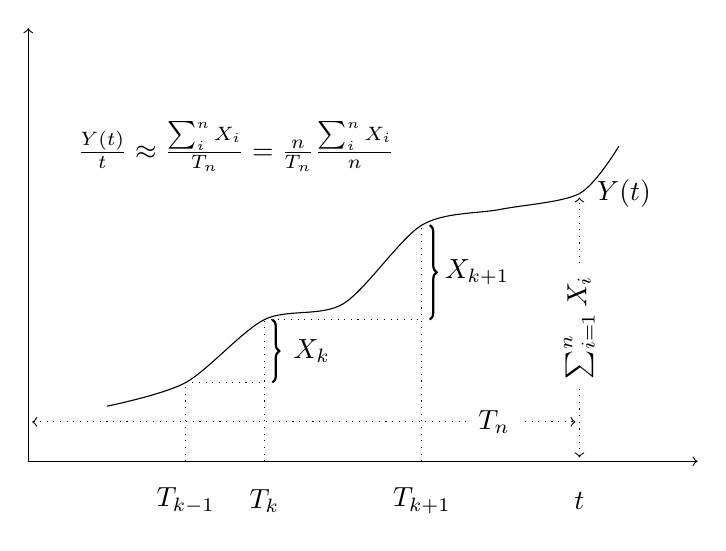
\begin{tikzpicture}[scale=1]
%axis
\draw[->] (0,0) -- coordinate (x axis mid) (8.5,0);
\draw[->] (0,0) -- coordinate (y axis mid) (0,5.5);
%\node[below=0.2cm] at (x axis mid) {$t$};

\draw plot [smooth] coordinates {(1,0.7) (2,1) (3,1.8) (4,2) (5,3) (6,3.2) (7, 3.4) (7.5,4.0)};
\node[right] at (7.1,3.4) {$Y(t)$};
\node at (7.,-0.5) {$t$};

\node at (2.,-0.5) {$T_{k-1}$};
\draw[dotted] (2,0)--(2,1);
\draw[dotted] (2,1)--(3,1);


\node at (3.,-0.5) {$T_{k}$};
\draw[dotted] (3,0)--(3,1.8);
\draw[dotted] (3,1.8)--(5,1.8);

\draw [
 thick,
 decoration={brace, mirror, raise=0.1cm },
 decorate
] (3,1) -- (3,1.8)
node[pos=0.5, xshift=0.6cm] {$X_k$}; 


\node at (5.,-0.5) {$T_{k+1}$};
\draw[dotted] (5,0)--(5,3);

\draw [
 thick,
 decoration={brace, mirror, raise=0.1cm },
 decorate
] (5,1.8) -- (5,3)
node[pos=0.5, xshift=0.7cm] {$X_{k+1}$}; 

\node[right] at (0.5,4) {$\frac{Y(t)}t \approx \frac{\sum_i^n X_i}{T_n} = \frac{n}{T_n} \frac{\sum_i^n X_i}n $};


\draw[dotted,<->, =stealth] (7,0.05)--(7,3.35) node[midway, rotate=90, fill=white] {$\sum_{i=1}^n X_i$};
\draw[dotted,<->, =stealth] (0.05,0.5)--(6.95,0.5) node[pos=0.85, fill=white] {$T_n$};
\end{tikzpicture}
\caption{A graphical `proof' of $Y=\lambda X$. Here $Y(t)/t\to Y$, $n/T_n\to \lambda$ and $n^{-1}\sum_i^n X_i \to X$. Observe that in the
 figure $X_k$ does not represent an inter-arrival time; instead it
 corresponds to the increment of (the graph of) $Y(t)$ between two
 consecutive epochs $T_{k-1}$ and $T_k$ at which $Y(t)$ is
 observed.}
 \label{fig:renewal}
\end{figure}

Let us use this theorem to understand the idea of `load' in a different way. 
Define the \recall{load} or \recall{utilization} as the limiting fraction of time the server is busy, i.e.,
\begin{equation*}
 \rho = \lim_{t\to\infty} \frac 1 t \int_0^t \1{L(s)>0} \d s.
\end{equation*}

\begin{exercise}\clabel{ex:l-162}
Use the renewal reward theorem to prove that $\rho = \lambda \E S$ for the rate-stable $G/G/1$ queue. 
\begin{hint}
 Define $Y(t) = \int_0^t \1{L(s)>0} \d s$ as the total amount of time the server has been busy up to the time $t$.
 Then take as epochs $T_k = D_k$ and use rate stability.
\end{hint}
\begin{solution}
 It is evident that $X_k = Y(D_k)-Y(D_{k-1})=S_k$, hence $X = \lim_{n\to\infty} n^{-1}\sum_{k=1}^n X_k = \E S$.
 Also $\lim_{t\to\infty} Y(t)/t=\rho$.
 Finally, in the relation $Y = \lambda X$, the $\lambda$ is $\delta$ since we consider departure epochs $T_k = D_k$, rather than $A_k$.
 By the renewal reward theorem $Y=\lambda X$ we get that $\rho = \delta \E S$.
 Finally, by rate-stability, the job arrival rate $\lambda = \delta$, hence $\rho = \lambda \E S$.
\end{solution}
\end{exercise}


\begin{exercise}\clabel{ex:l-163}
 We can derive the relation $\rho = \lambda \E S$ in a somewhat more direct way by considering the fact that
\begin{equation*}
 \sum_{k=1}^{A(t)} S_k \geq \int_0^t \1{L(s)>0} \d s \geq \sum_{k=1}^{D(t)} S_k.
\end{equation*}
Explain this, and complete the argument.
\begin{solution}
Observe that
since $t$ can lie half way a service interval and $A(t) \geq D(t)$. As
$A(t)\to \infty$ as $t\to\infty$,
\begin{equation*}
 \lim_{t\to\infty} \frac 1 t\sum_{k=1}^{A(t)} S_k = 
 \lim_{t\to\infty} \frac{A(t)}t \frac{1}{A(t)} \sum_{k=1}^{A(t)} S_k = 
 \lim_{t\to\infty} \frac{A(t)}t \cdot \lim_{t\to\infty}\frac{1}{A(t)} \sum_{k=1}^{A(t)} S_k = \lambda \E S.
\end{equation*}
Applying similar limits to the other inequality gives
\begin{equation*}
\lambda \E S \geq \rho \geq \delta \E S.
\end{equation*}
Hence, if the system is rate-stable, $\delta=\lambda$, and then $\rho = \lambda \E S$. 

Note that this is in fact the same argument as that underlies the renewal reward theorem. Henceforth we will just use the renewal reward theorem. 
\end{solution}
\end{exercise}



\opt{solutionfiles}{
\Closesolutionfile{hint}
\Closesolutionfile{ans}
\subsection*{Hints}
\input{hint}
\subsection*{Solutions}
\input{ans}
}
%\clearpage


%%% Local Variables:
%%% mode: latex
%%% TeX-master: "../companion"
%%% End:

\input{tex_files/levelcrossing.tex}
\section{Poisson Arrivals See Time Averages}
\label{sec:poisson-arrivals-see}


\opt{solutionfiles}{
\subsection*{Theory and Exercises}
\Opensolutionfile{hint}
\Opensolutionfile{ans}
}

Suppose the following limit exists:
\begin{equation}\label{eq:jaap}
 \pi(n) 
= \lim_{m\to\infty} 
\frac1m\sum_{k=1}^m \1{L(A_k-) = n},
\end{equation}
then $\pi(n)$ is the long-run fraction of jobs that observe $n$ customers in the system at the moment an arbitrary job arrives.
It is natural to ask whether $\pi(n)$ and $p(n)$, as defined by~\cref{eq:p(n)}, are related, that is, whether what customers see upon arrival is related to the time-average behavior of the system.
In this section we will derive the famous \recall{Poisson arrivals see time averages} (\recall{PASTA}) condition that ensures that $\pi(n)=p(n)$ if jobs arrive in accordance with a Poisson process.


%We can make some progress by rewriting $\pi(n)$ in the following way.
Since $A(t)\to \infty$ as $t\to\infty$, it is reasonable that (see~\cref{ex:18} for a proof)
\begin{equation}\label{eq:132}
 \begin{split}
 \pi(n) &= \lim_{t\to\infty} \frac1{A(t)}\sum_{k=1}^{A(t)} \1{L(A_k-) = n} 
= \lim_{t\to\infty} \frac1{A(t)}\sum_{k=1}^\infty \1{A_k \leq t, L(A_k-) = n} \\
 &= \lim_{t\to\infty} \frac{A(n,t)}{A(t)},
 \end{split}
\end{equation}
where we use~\cref{eq:19} in the last row. But, with~\cref{eq:3}, 
\begin{equation}\label{eq:1333}
 \frac{A(n,t)}{t} 
= \frac{A(t)}t \frac{A(n,t)}{A(t)}
\to \lambda \pi(n), \quad\text{as } t \to \infty, 
\end{equation}
while by ~\cref{eq:21}, 
\begin{equation*}
\frac{A(n,t)}t = \frac{A(n,t)}{Y(n,t)}\frac{Y(n,t)}t \to \lambda(n) p(n), \quad\text{as } t \to \infty.
\end{equation*}
Thus
\begin{equation}\label{eq:13}
\lambda \pi(n) = \lambda(n) p(n).
\end{equation}
This leads to our final result:
\begin{equation*}
 \lambda(n) = \lambda \iff \pi(n) = p(n).
\end{equation*}
This means that if the arrival rate does not depend on the state of the system, i.e., $\lambda(n)=\lambda$, the sample probabilities $\{\pi(n)\}$ are equal to the time-average probabilities $\{p(n)\}$. 
In other words, the customer perception at arrival moments is the same as the server perception.

As the next exercises show, this property is not satisfied in general.
However, when the arrival process is Poisson we have that $\lambda(n)=\lambda$.
This fact is called \emph{PASTA: Poisson Arrivals See Time Averages}.
Thus, for the $M/M/1$ queue in particular,
\begin{equation*}
 \pi(n) = p(n) = (1-\rho)\rho^n.
\end{equation*}

\begin{exercise}\clabel{ex:8} 
Show for the case of~\cref{ex:112} that $\pi(0)=1$ and $\pi(n)=0$, for $n>0$.
\begin{solution}
  All arrivals see an empty system.
  Hence $A(0,t)/A(t) \approx (t/2)/(t/2) = 1$, and $A(n,t)=0$ for $n>0$.
  Thus, $\pi(0) = \lim_{t\to\infty} A(0,t)/A(t) = 1$ and $\pi(n)=0$ for $n>0$.
  Recall from the other exercises that $p(0)=1/2$.
  Hence, statistics as obtained via time averages are not necessarily the same as statistics obtained at arrival moments (or any other point process).
\end{solution}

\end{exercise}

\begin{exercise}\clabel{ex:l-152}
 Check that~\cref{eq:13} holds for the system of~\cref{ex:8}.
\begin{solution}
From the relevant previous exercises, $\lambda = \lim_{t\to\infty} A(t)/t = 1/2$. $\lambda(0)=1$, $p(0)=1/2$, and $\pi(0)=1$. Hence,
\begin{equation*}
 \lambda \pi(0) = \lambda(0) p(0) \implies \frac 1 2 \times 1 = 1\times \frac 1 2.
\end{equation*}
For $n>0$ it's easy, everything is 0.
\end{solution}
\end{exercise}





With the above reasoning, we can also establish a relation between $\pi(n)$ and the statistics of the system as obtained by the departures.
Define, analogous to~\cref{eq:132}, 
\begin{equation}
 \label{eq:33}
 \delta(n) = \lim_{t\to\infty} \frac{D(n,t)}{D(t)}
\end{equation}
as the long-run fraction of jobs that leave $n$ jobs \emph{behind}.
From~\cref{eq:15},
\begin{equation*}
\frac{A(t)}t \frac{A(n,t)}{A(t)} = \frac{A(n,t)}t \approx \frac{D(n,t)}t 
= \frac{D(t)}t \frac{D(n,t)}{D(t)}.
\end{equation*}
Taking limits at the left and right, and using~\cref{eq:28}, we obtain for (queueing) systems in which customers arrive and leave as single units that
\begin{equation}
 \label{eq:36}
 \lambda \pi(n) = \delta \delta(n).
\end{equation}
Thus, if the system is rate-stable and transitions occur one-by-one, the statistics obtained by arrivals is the same as statistics obtained by departures, i.e., 
\begin{equation}
 \label{eq:39}
\lambda = \delta \iff \pi(n) = \delta(n).
\end{equation}

\begin{exercise}\clabel{ex:pasta-26}
 For the $G/G/1$ queue, prove that the fraction of jobs that see $n$ jobs in the system upon arrival is the same as the fraction of departures that leave $n$ jobs behind.
 What condition have you used to prove this?
%\item Motivate that for the $G/M/1$, $\delta(n) = p(n)$, i.e., departures see time averages. 
\begin{hint}
Note that~\cref{eq:97}  does not depend on the distribution of the inter-arrival or service times.
\end{hint}
\begin{solution}
 All follows straightaway from the definitions in the main text.
 In the $G/G/1$ queue jobs arrive and depart in single units.
 Then, from~\cref{eq:97},
 \begin{equation*}
 \frac{A(t)}{t}\frac{A(n,t)}{A(t)} \approx 
 \frac{D(t)}{t}\frac{D(n,t)}{D(t)}. 
 \end{equation*}
 The left-hand side goes to $\lambda \pi(n)$ as $t\to\infty$, and
 the right-hand side to $\delta \delta(n)$. Use the fact that we
 always assume, implicitly, that the system is stable, so that
 $\lambda = \delta$. As a consequence $\delta(n) = \pi(n)$ for the $G/G/1$ queue.
\end{solution}
\end{exercise}


\begin{exercise}\clabel{ex:26}
 When $\lambda\neq \delta$, is $\pi(n)\geq \delta(n)$? 
\begin{hint}
 Use that $\lambda \geq \delta$ always holds. Thus, when $\lambda \neq \delta$, it must be that $\lambda > \delta$. What are the consequences of this inequality; how does the queue length behave as a function of time?
\end{hint}
\begin{solution}
 The assumptions lead us to conclude that $\lambda > \delta$. As a consequence, the queue length must increase in the long run (jobs come in faster than they leave). Therefore, $A(n,t)/t \to 0$ for all $n$, and also $D(n,t)/t\to 0$. Consequently, $\pi(n) = \delta(n) = 0$, which is the only sensible reconciliation with~\cref{eq:36}. 
\end{solution}
\end{exercise}

\begin{extra}\clabel{ex:909}
Show that 
\begin{equation*}
\lambda \pi(n) = \lambda(n) p(n) = \mu(n+1) p(n+1) = \delta \delta(n).
\end{equation*}
What is the important condition for this to be true?
\begin{hint}
Check all definitions of $Y(n,t)/t$ and so on.
\end{hint}
\begin{solution}
 The important condition is that transitions occur as single
 steps. In other words, the relation is true for processes with
 \recall{one-step transitions}, i.e., when $|A(n,t) - D(n,t)|\leq 1$.
 In that case, 
\begin{align*}
 \frac{A(n,t)}{t} &= \frac{A(n,t)}{A(t)} \frac{A(t)}{t} \to \pi(n) \lambda\\
 \frac{A(n,t)}{t} &= \frac{A(n,t)}{Y(n,t)} \frac{Y(n,t)}{t} \to \lambda(n)p(n)\\
 \frac{D(n,t)}{t} &= \frac{D(n,t)}{Y(n+1,t)} \frac{Y(n+1,t)}{t} \to \mu(n+1)p(n+1)\\
 \frac{D(n,t)}{t} &= \frac{D(n,t)}{D(t)} \frac{D(t)}{t} \to \delta(n)\delta. \\
\end{align*}
\end{solution}
\end{extra}

\begin{extra}\clabel{ex:58}
 Use PASTA and the balance equations of the $M/M/1$ queue to derive that $(\lambda + \mu) \pi(n) = \lambda \pi(n-1) + \mu \pi(n+1)$.
\begin{hint}
 Consider some state $n$ (not a level) and count all transitions that `go in and out of' this state.
 Specifically, $A(n,t) + D(n-1,t)$ counts all transitions out of state $n$: $A(n,t)$ counts the number of arrivals that see $n$ in the system upon arrival, hence immediately after such arrivals the system contains $n+1$ jobs; likewise, $D(n-1,t)$ counts all jobs that leave $n-1$ jobs behind, hence immediately before such jobs depart the system contains $n$ jobs.
 In a similar way, $A(n-1,t) + D(n,t)$ counts all transitions into state $n$ (Recall once again, $D(n,t)$ counts the jobs that leave $n$ behind.
 Hence, when such departures occur, state $n$ is entered).
 Now use that `what goes in must go out'.
\end{hint}
\begin{solution}
By the hint, the difference between the `out
 transitions' and the `in transitions' is at most 1 for all $t$. Thus, we can write
 \begin{align*}
\text{transitions out } &\approx \text{transitions in } \iff \\
 A(n,t) + D(n-1,t) &\approx A(n-1,t) + D(n,t) \iff \\
 \frac{A(n,t) + D(n-1,t)}t &\approx \frac{A(n-1,t) + D(n, t)}t \iff \\
 \frac{A(n,t)}t + \frac{D(n-1,t)}t &\approx \frac{A(n-1,t)}t + \frac{D(n,t)}t.
 \end{align*}
Using the ideas of~\cref{sec:level-cross-balance} this becomes for $t\to\infty$, 
\begin{equation*}
 (\lambda(n) +\mu(n))p(n) = \lambda(n-1)p(n-1) + \mu(n+1)p(n+1).
\end{equation*}
Since we are concerned here with the $M/M/1$ queue we have that
$ \lambda(n) = \lambda$ and $\mu(n) = \mu$, and using PASTA we have
that $p(n) = \pi(n)$. We are done.
\end{solution}
\end{extra}





\begin{exercise}\clabel{ex:18}
 There is a subtle problem in the transition from~\cref{eq:jaap} to~\cref{eq:132} and the derivation of~\cref{eq:1333}: $\pi(n)$ is defined as a limit over arrival epochs while in $A(n,t)/t$ we take the limit over time.
 Now the observant reader might ask why these limits should relate at all.
 Use the renewal reward theorem to show that~\cref{eq:132} is valid.
\begin{hint}
Check that the conditions of the renewal reward theorem are satisfied in the above proof of~\cref{eq:1333}. Then define 
\begin{align*}
 Y(t) &:= A(n,t) = \sum_{k=1}^{A(t)} \1{L(A_k-) = n} \\
X_k &:= Y(A_k) - Y(A_{k-1}) = A(n, A_k) - A(n, A_{k-1}) = \1{L(A_k-)=n}.
\end{align*}

\end{hint}
\begin{solution}
First we check the conditions. The counting process here is $\{A(t)\}$ and the epochs at which
 $A(t)$ increases are $\{A_k\}$. By assumption, $A_k\to\infty$,
 hence $A(t)\to\infty$ as $t\to\infty$. Moreover, by assumption
 $A(t)/t \to \lambda$. Also $A(n,t)$ is evidently non-decreasing and
 $A(n,t)\to\infty$ as $t\to\infty$.


From the definitions in the hint, 
\begin{equation*}
X= \lim_{m\to\infty} \frac 1 m \sum_{k=1}^m X_k =\lim_{m\to\infty} \frac 1 m \sum_{k=1}^m \1{L(A_k-)=n} = \pi(n).
\end{equation*}
Since $Y=\lim_{t\to\infty} Y(t)/t = \lim_{t\to\infty} A(n,t)/t$ it follows from the renewal reward theorem that
\begin{equation*}
 Y=\lambda X \implies \lim_{t\to\infty} \frac{A(n,t)} t = \lambda X = \lambda \pi(n).
\end{equation*}
Thus,~\cref{eq:1333} follows from the renewal reward theorem.
\end{solution}
\end{exercise}



\opt{solutionfiles}{
\Closesolutionfile{hint}
\Closesolutionfile{ans}
\subsection*{Hints}
\input{hint}
\subsection*{Solutions}
\input{ans}
}
%\clearpage


%%% Local Variables:
%%% mode: latex
%%% TeX-master: "../companion"
%%% End:

\section{Little's Law}
\label{sec:littles-law}

There is an important relation between the average time $\E W$ a job
spends in the system and the long-run time-average number $\E L$ of jobs
that is contained in the system, which is called \emph{Little's law}:
\begin{equation}\label{eq:53}
 \E L = \lambda \E W.
\end{equation}
Part of the usefulness of Little's law is that it applies under very general conditions to all input-output systems, whether the system is a queueing system or an inventory system or some much more general system.
Hence, we will apply Little's law often in the forthcoming sections.
The aim of this section is to prove this law.

\opt{solutionfiles}{
\subsection*{Theory and Exercises}
\Opensolutionfile{hint}
\Opensolutionfile{ans}
}


%\Cref{ex:62} provides a proof of this under some simple conditions.

We start by defining a few intuitively useful concepts. From~\cref{eq:14}, we see that
\begin{equation*}
\frac 1 t\int_0^t L(s)\, \d s = \frac 1 t\int_0^t (A(s)-D(s)) \, \d s
\end{equation*}
is the time-average of the number of jobs in the system during
$[0,t]$.
% Observe once again from the second equation that
% $\int_0^t L(s)\,\d s$ is the area enclosed between the graphs of $A(s)$
% and $D(s)$.
Next, the waiting time of the $k$th job is the time between the moment the
job arrives and departs, that is, 
\begin{equation*}
 W_k = \int_0^\infty \1{A_k \leq s < D_k}\,\d s.
\end{equation*}
\cref{fig:atltdt}  relates $W_k$ to $L(t)$.

Consider a departure time $T$ at which the system is empty so that $A(T) = D(T)$.
%as at time $T$ all jobs that arrived up to $T$ also have left.
%As for all jobs $k\leq A(T)$ we have that $D_k \leq T$, we can replace the integration bounds in the above expression for $W_k$ by
Then, for $k\leq A(T)$, 
\begin{equation*}
 W_k = \int_0^T \1{A_k \leq s < D_k}\,\d s,
\end{equation*}
and for $s\leq T$,
\begin{equation*}
L(s) = \sum_{k=1}^\infty \1{A_k \leq s < D_k} = \sum_{k=1}^{A(T)}\1{A_k \leq s < D_k}.
\end{equation*}



\begin{extra}\clabel{ex:59}
 Show that 
\begin{equation*}
 \int_0^T L(s)\, \d s = \sum_{k=1}^{A(T)} W_k.
\end{equation*}
\begin{hint}
 Substitute the definition of $L(s)$ in the left-hand side, then reverse the integral and summation.
\end{hint}
\begin{solution}
\begin{equation*}
 \begin{split}
 \int_0^T L(s)\, \d s & = \int_0^T \sum_{k=1}^{A(T)} \1{A_k \leq s < D_k}\, \d s \\
& = \sum_{k=1}^{A(T)}\int_0^T \1{A_k \leq s < D_k}\, \d s = \sum_{k=1}^{A(T)} W_k.
 \end{split}
\end{equation*}
\end{solution}
\end{extra}


\begin{extra}
Observe that the area between the graphs of $A(s)$ and $D(s)$ must
be equal to the total waiting time spent by all jobs in the system
until $T$. Use this to provide a graphical interpretation of the proof of Little's law.
\begin{hint}
 Make a drawing of $A(t)$ and $D(t)$ until time $T$, i.e., the
 first time the system is empty. Observe that $A(t)-D(t)$ is the number of jobs in the system. Take some level $k$, and compute $A_k = A^{-1}(k)$ and $D_k = D^{-1}(k)$. Observe that $D_k - A_k = D^{-1}(k) - A^{-1}(k)$ is the waiting time of job $k$.
\end{hint}
\begin{solution}
  The area enclosed between the graphs of $A(t)$ and $D(t)$ until $T$ can be `chopped up' in two ways: in the horizontal and in the vertical direction.
  (Please make the drawing as you go along\ldots) A horizontal line between $A(t)$ and $D(t)$ corresponds to the waiting time of a job, while a vertical line corresponds to the number of jobs in the system at time $t$.
  Now adding all horizontal lines (by integrating along the $y$-axis) makes up the total amount of waiting done by all the jobs until time $T$.
  On the other hand, adding the vertical lines (by integrating along the $x$-axis) is equal to the summation of all jobs in the system.
  Since the area is the same no matter whether you sum it in the horizontal or vertical direction:
 \begin{equation*}
 \sum_{k=1}^{A(T)} W_k = \text{enclosed area} = \int_0^T (A(t)-D(t))\,dt. 
 \end{equation*}
 Dividing both sides by $A(T)$ gives
 \begin{equation*}
\frac{1}{A(T)} \sum_{k=1}^{A(T)} W_k =\frac{1}{A(T)} \int_0^T (A(t)-D(t))\,dt. 
 \end{equation*}

 Finally, observe that this equality holds between any two times
 $T_i, T_{i+1}$, where times $\{T_i\}$ are such that
 $A(T_i)=D(T_i)$. Then, as $T_i\to \infty$, which we assumed from
 the on-set, $\frac{1}{A(T_i)} \sum_{k=1}^{A(T_i)} W_k\to \E W$,
 and
 \begin{equation*}
\frac{T_i}{A(T_i)}\frac{1}{T_i} \int_0^{T_i} (A(t)-D(t))\,dt \to \lambda^{-1} \E L.
 \end{equation*}
Hence, Little's law follows.
\end{solution}
\end{extra}

\begin{exercise}\clabel{ex:62}
 Prove Little's law under the assumptions that $A(T_i) = D(T_i)$ for an infinite number of times $\{T_i\}$ such $T_i\to\infty$ and that all limits exist. 
\begin{hint}
In  the result of~\cref{ex:59},  divide both sides by $T$. At the right-hand side use that $1/T = A(T)/T \cdot 1/A(T)$. Take limits.
\end{hint}
\begin{solution}
  First solve~\cref{ex:59}. Then,
\begin{equation*}
 \frac 1 T \int_0^T L(s)\, \d s = \frac{A(T)} T \frac{1}{A(T)} \sum_{k=1}^{A(T)} W_k.
\end{equation*}
Assuming there are an infinite number of times
$0\leq T_i<T_{i+1}<\cdots$, $T_i\to\infty$, at which $A(T_i) = D(T_i)$
and the following limits exist
\begin{align*}
\frac 1 T \int_0^T L(s)\, \d s &\to \E L,&
\frac{A(T_i)}{T_i} &\to \lambda, &
\frac{1}{A(T_i)} \sum_{k=1}^{A(T_i)} W_k &\to \E W,
\end{align*}
we obtain Little's law.

\end{solution}
\end{exercise}


\begin{extra}\clabel{ex:42}
  Use the (physical) dimensions of the components of Little's law to check that $\E{W} \neq \lambda \E{L}$.
  (With this check, you can prevent making an often-made mistake.)
\begin{hint}
Checking the dimensions in the formula prevents painful mistakes.
\end{hint}
\begin{solution}
 Sometimes (often?) students memorize Little's law in the wrong
 way. Thus, as an easy check, use the dimensions of the concepts:
 $\E L$ is an average \emph{number}, $\lambda$ is a \emph{rate},
 i.e., \emph{numbers per unit time}, and $\E W$ is waiting
 \emph{time}. 
\end{solution}
\end{extra}



\begin{extra}\clabel{ex:37}
 Consider the server of the $G/G/1$ queue as a system by itself.
 The time jobs stay in this system is $\E S$, and jobs arrive at rate $\lambda$.
 Use  Little's law to conclude that  $\lambda \E S = \rho := \lim_{t\to\infty} t^{-1}\int_0^t L_S(s)\d s$.
\begin{solution}
 The arrival rate at the server must be $\lambda$ and the time a job remains at the server is $\E S$.
 The fraction of time the server is busy is precisely the fraction of time there is a job present at the server.
 Thus, applying Little's law to the server itself, we see that $\rho = \E{L_S} = \lambda \E S$.
\end{solution}
\end{extra}


\begin{extra}\clabel{ex:43}
 For a given single-server queueing system the average number of customers in the system is $\E L = 10$, customers arrive at rate $\lambda=5$ per hour and are served at rate $\mu=6$ per hour.
 What is the average time customers spend in the system?
\begin{hint}
Start with checking the units when applying Little's law.
\end{hint}
\begin{solution}
 \begin{equation*}
 \E W = \E L/\lambda = 10/\lambda = 10/5 = 2.
 \end{equation*}
\end{solution}
\end{extra}

\begin{exercise}\clabel{ex:44}
 For a given single-server queueing system the average number of customers in the system is $\E L = 10$, customers arrive at rate $\lambda=5$ per hour and are served at rate $\mu=6$ per hour.
 Suppose that at the moment you join the system, the number of customers in the system is 10.
 What is your expected time in the system?
\begin{solution}
If you arrive at a queueing system, you first have to wait until the job in service is finished. Then you need to wait until the 9 jobs in queue are finished. This takes, in expectation, $9/\mu$. (Recall, 1 job is in service at the moment you arrive, so 9 are in queue.) Assuming that service times are exponential, so that, by the memoryless property, the remaining service time of the job in service is still $\E S$ when you arrive, you spend $10/\mu + 1/\mu = 11/6 \neq 2$. (To account for the last $+1/\mu$, observe that yourself also have to be served to compute the time you spend in the system.)


Now in this question, it is \emph{given} that the system
 length is 10 at the moment of arrival. However, $L$ as `seen' upon arrival by this
 given customer is in general not the same as the time-average $\E{L}$.

Thus, Little's law need not hold at all moments in time; it is a statement about \emph{averages}.
\end{solution}

\end{exercise}

With the PASTA property and Little's law it becomes quite easy to derive expressions for the average queue length and waiting times for the $M/M/1$ queue.
The average waiting time $\E W$ in the entire system is the expected time in queue plus the expected time in service, i.e.,
\begin{equation}\label{eq:78}
 \E W = \E{W_Q}+ \E S.
\end{equation}
By the PASTA property we have for the $M/M/1$ queue that
\begin{equation}\label{eq:wqes}
 \E{W_Q} = \E L \E S.
\end{equation}


\begin{exercise}\clabel{ex:l-215}
Use Little's law to show for the $M/M/1$ queue that 
 \begin{align*}
 \E W &= \frac{\E S}{1-\rho}, & \E L &= \frac\rho{1-\rho}, \\
 \E{L_Q} &= \frac{\rho^2}{1-\rho}, & \E{L_s} &= \rho.
 \end{align*}
\begin{hint}
 Combine~\cref{eq:78,eq:wqes} and apply Little's law. 
\end{hint}
\begin{solution}
\begin{align*}
 \E W &= \E L \E S + \E S = \lambda \E W \E S + \E S= \rho \E W + \E S, \\
 \E L &= \lambda \E W = \frac{\lambda \E S}{1-\rho} = \frac\rho{1-\rho}, \\
 \E{W_Q} &= \E W - \E S = \frac{\E S}{1-\rho} - \E S = \frac{\rho}{1-\rho} \E S,\\
 \E{L_Q} &= \lambda \E{W_Q} = \frac{\rho^2}{1-\rho}, \\
 \E{L_s} &= \E L - \E{L_Q} = \frac{\rho}{1-\rho} - \frac{\rho^2}{1-\rho} = \rho, 
\end{align*}
\end{solution}
\end{exercise}

\begin{exercise}\clabel{ex:l-216}
Why is~\cref{eq:wqes} \emph{not} true in general for the $M/G/1$ queue? 
\begin{solution}
 By the memoryless property of the (exponential) distributed service times of the $M/M/1$ queue, the duration of a job in service, if any, is $\Exp(\mu)$ also at an arrival moment.
 Therefore, at an arrival moment, all jobs in the system (whether in service or not) have the same expected duration.
 Hence, the expected time to spend in queue is the expected number of jobs in the system times the expected service time of each job, i.e., $\E{W_q} = \E L \E S$.
 Note that we use PASTA to see that the expected number of jobs in the system at an arrival is $\E{L}$.
 For the $M/G/1$ queue, the job in service (if any) does not have the same distribution as a job in queue.
 Hence, the expected time in queue is not $\E L \E S$.
\end{solution}
\end{exercise}




In the above proof of Little's law we assumed that there is a sequence of moments $\{T_k, k=0,1,\ldots\}$ at which the system is empty and such that $T_k < T_{k+1}$ and $T_k \to \infty$.
However, in many practical queueing situations the system is never empty.
Thus, to be able to apply Little's law to such more general situations we should slacken the assumption that such a sequence exists.
The aim of this set of questions is to find an educated guess for a more general assumption under which Little's law can hold.


\begin{exercise}\clabel{ex:l-220}
 Motivate in words (or with a derivation, if you prefer this) why the following is true:
 \begin{equation*}
 \sum_{k=1}^{A(t)} W_k \geq \int_0^t L(s) \d s \geq \sum_{k=1}^{D(t)} W_k.
 \end{equation*}
\begin{solution}
 Intuitively, the left term is all the work that arrived up to time $t$, the middle term is all the work that has been processed, and the right term all the work that left.
 Any job that that is half way its service counts for full at the left, for half in the middle expression, and not in the right.

 More formally, for any job $k$ and time $t$, we have $W_k \1{A_k \leq t} \geq \int_0^t \1{A_k \leq s < D_k } \d s \geq W_k \1{D_k \leq t}$. (To see this, fix $k$, and check the three cases $t < A_k, A_k \leq t < D_k, D_k < t$.) Then,
 \begin{equation*}
 \sum_{k=1}^\infty W_k \1{A_k \leq t} \geq \int_0^t \sum_{k=1}^\infty \1{A_k \leq t < D_k} \d s \geq \sum_{k=1}^\infty W_k \1{D_k \leq t}. 
 \end{equation*}
 Finally, note that $ \sum_{k=1}^\infty W_k \1{A_k \leq t} = \sum_{k=1}^{A(t)} W_k$ and $ \sum_{k=1}^\infty W_k \1{D_k \leq t} = \sum_{k=1}^{D(t)} W_k$, and use the definition of $L(s)$.
\end{solution}
\end{exercise}

\begin{exercise}\clabel{ex:l-221}
Take suitable limits (and assume all these limits exist) to show that 
 \begin{equation*}
\lambda \E W \geq \E L \geq \delta \E W.
 \end{equation*}
 Make explicit all the points where you use the strong law of large numbers.
\begin{solution}
 \begin{equation*}
 \lim_{t\to\infty} \frac{A(t)}{t}\frac 1{A(t)}\sum_{k=1}^{A(t)} W_k \geq \lim_{t\to \infty} \frac 1 t \int_0^t L(s) \d s \geq \lim_{t\to\infty} \frac{D(t)}{t}\frac 1{D(t)} \sum_{k=1}^{D(t)} W_k. 
 \end{equation*}
 We use the strong law of large numbers to conclude that limits converges to $n^{-1} \sum_{k=1}^n W_k \to \E W$, and we assume that $\{W_k, k\geq N\}$ forms a sequence of i.i.d.
 random variables for $N$ sufficiently large.
\end{solution}
\end{exercise}


\begin{exercise}\clabel{ex:l-222}
 Suppose that $A(t) = \lambda t$ and $D(t)= [A(t) - 10]^+$.
 Explain that for this system the above assumption on $\{T_k\}$ is violated. Show that Little's law is still true.
\begin{solution}
 When $t>10$, $L(t) = 10$.
 Hence the system is never empty.
 Since still $\delta=\lim_{t\to\infty} D(t)/t = \lambda$, and $\lim_{n\to \infty} n^{-1}\sum_{k=1}^n W_k$ exists, Little's law follows.
\end{solution}
\end{exercise}

\begin{exercise}\clabel{ex:l-223}
 Based on the above formulate an educated guess for more general conditions under which Little's law holds.
 (You don't have to prove Little's law under your condition; postpone that to after the exam.)
\begin{solution}
We seem to need that $\lambda = \delta$ and that $\lim_{n\to \infty} n^{-1}\sum_{k=1}^n W_k$ exists. 
\end{solution}
\end{exercise}




\opt{solutionfiles}{
\Closesolutionfile{hint}
\Closesolutionfile{ans}
\subsection*{Hints}
\input{hint}
\subsection*{Solutions}
\input{ans}
}

%\clearpage



%%% Local Variables:
%%% mode: latex
%%% TeX-master: "../companion"
%%% End:

\section{Graphical Summary}

We finish this chapter with providing two summaries in graphical form to clarify how all concepts developed in this chapter relate.

\begin{figure}[p]
 \centering

 \begin{tikzpicture}[node distance = 2.5cm]

\tikzset{
 %Define standard arrow tip
 >=stealth',
 %Define style for boxes
 % Define arrow style
 pil/.style={
 ->,
 thick,
 shorten <=2pt,
 shorten >=2pt,}
}
\tikzstyle{block} = [rectangle, draw,text centered, rounded corners, minimum height=3em]

 % nodes
 \node [block, text width=5.5cm, align=center] (level) {LEVEL CROSSING: Counting up- and down-crossings};
\node[block, below=1cm of level] (An) {$|A(n,t)-D(n,t)|\leq 1$}
edge[pil,<-] (level); 

\node[block, left=1.5cm of An] (A) {$A(t)-D(t)=L(t)$} 
edge[pil,<-] (level); 

\node[block, right=1.5cm of An] (Anm) {$|A(m,n,t)-D(n,t)|\leq 1$}
edge[pil,<-] (level); 

\node[block, below=1cm of A] (At) {$\frac{A(t)}t \approx \frac{D(t)}t$ if $\frac{L(t)}t \to 0$} 
edge[pil,<-] (A); 

\node[block, below=1.5cm of At] (lambda) {$\lambda=\delta$} 
edge[pil,<-] node[fill=white] {$t\to\infty$} (At); 

\node[block, below=1cm of An] (AnDn) {$\frac{A(n,t)}t\approx\frac{D(n,t)}t$}
edge[pil,<-] (An); 

\node[block, below=1.5cm of AnDn] (AnDn2) {$\frac{A(n,t)}{Y(n,t)}\frac{Y(n,t)}t\approx\frac{D(n,t)}{Y(n+1)}\frac{Y(n+1)}t$}
edge[pil,<-] (AnDn); 

\node[block, below=1.5cm of AnDn2, text width=4cm] (lp) {Level Crossing: \\
$\lambda(n)p(n) = \mu(n+1)p(n+1)$}
edge[pil,<-] node[fill=white] {$t\to\infty$} (AnDn2); 

\node[block, below=1cm of lp, text width=3cm] (poisson) {Poisson: \\
$\lambda=\lambda(n)$, \\
$\mu=\mu(n)$}
edge[pil,<-] (lp);

\node[block, below=1cm of poisson, text width=4cm] (mm1) {$M/M/1$, $M/M/c$, $M/M/c/k$, \ldots} edge[pil,<-] (poisson);
;

\node[block, right=0.6cm of lp, text width=5cm, align=center] (batch) {Recursion: \\ $\lambda\sum_{m=0}^nG(n-m)p(m) = \mu(n+1)p(n+1)$}
edge[pil,<-] node[fill=white] {$t\to\infty$} (Anm); 

\node[block, right=2.3cm of mm1] (batch2) {$M^X/M/1$}
edge[pil,<-] (poisson)
edge[pil,<-] (batch); 


\node[block, below=1cm of mm1, text width=4.5cm] (perf) {Performance
 measures:
$\E L= \sum_{n=0}^\infty n p(n)$, $\P{L\geq m}$, \ldots} 
edge[pil,<-] (mm1)
edge[pil,<-] (batch2);

\node[block, below=1.5cm of lambda] (pasta1) {$\frac{A(t)}t\frac{A(n,t)}{A(t)} = \frac{A(n,t)}{Y(n,t)}\frac{Y(n,t)}t$} 
edge[pil,<-] (AnDn2)
edge[pil,<-,bend left=20] (At.south west)
;

\node[block, below=1.5cm of pasta1] (pasta2) {$\lambda \pi(n) = \lambda(n)p(n)$} 
edge[pil,<-] node[fill=white] {$t\to\infty$} (pasta1);

\node[block, below=1.5cm of pasta2, text width=3cm] (pasta3) {PASTA: $\pi(n) = p(n)$} 
edge[pil,<-] (poisson)
edge[pil,<-] (pasta2)
edge[pil,->] (perf);

\end{tikzpicture}
 \caption{With level-crossing arguments we can derive a number of
 useful relations. This figure presents an overview of these
 relations that we derive in this and the next sections.}
\label{fig:summaries}
\end{figure}


%%% Local Variables:
%%% mode: latex
%%% TeX-master: "../companion"
%%% End:


\chapter{Exact Queueing Models}
\label{cha:analytical-models}

In this chapter we focus on developing analytic models for various queueing systems in steady-state.
As a reminder, we keep the discussion in these notes mostly at an intuitive level, and refer to \cite{el-taha98:_sampl_path_analy_queuein_system} for proofs and further background.

\input{tex_files/mm1.tex}
\section
{$M(n)/M(n)/1$ Queue}
%{$\mathbf{M(n)/M(n)/1}$ Queue}
\label{sec:mnmn1}

As it turns out, many more single-server queueing situations than the $M/M/1$ queue can be analyzed by making a judicious choice of $\lambda(n)$ and $\mu(n)$ in the level-crossing equations~\cref{eq:25}.
For these queueing systems, we just present the results.
In first set of exercises are somewhat technical; we ask you to derive the formulas---the main challenge is not to make computational errors.
The second set of exercises shows how the combination of PASTA and Little's law allows us to analyze an astonishingly large number of non-trivial practical queueing situations.

\opt{solutionfiles}{
\subsection*{Theory and Exercises}
\Opensolutionfile{hint}
\Opensolutionfile{ans}
}


It is important to realize that the inter-arrival times and service times need to be memoryless for the analysis below; the rates, however, may depend on the number of jobs in the system. Specifically, we require that for all $s$ and $t$,
\begin{equation*}
 \P{A_{A(t)+1} \leq t+s \given L(t) = n} = 1-e^{-\lambda(n) s},
\end{equation*}
where we use that $A_{A(t)}+g$ is the arrival time of the next job after time $t$.
Similarly, we assume for all $t$ and $s$,
\begin{equation*}
 \P{D_{D(t)+1} \leq t+s \given L(t)=n} = 1-e^{-\mu(n) s}.
\end{equation*}


\begin{exercise}\clabel{ex:l-244}
 Model the $M/M/1/K$ queue in terms of an $M(n)/M(n)/1$ queue and compute $p(K)$, i.e., the fraction of time that the system is full.
\begin{hint}
 Take $\lambda(n) = \lambda \1{n < K}$, $\mu(n) = \mu$, use the equations around~\cref{eq:38}.
\end{hint}
\begin{solution}
Note that 
\begin{equation*}
1 = \sum_{i=0}^K p(i) = p(0)\sum_{i=0}^K \rho^i = p(0) \frac{1-\rho^{K+1}}{1-\rho}. 
\end{equation*}
Thus,
\begin{subequations}\label{eq:8}
 \begin{align}
p(n) &= \frac{\rho^n}G, \quad 0\leq n \leq K,\\
p(K) &= \frac{1-\rho}{1-\rho^{K+1}} \rho^K.
\end{align}
\end{subequations}
\end{solution}
\end{exercise}

\begin{extra}\clabel{ex:40}
 Show that as $K\to\infty$, the performance measures of the $M/M/1/K$ converge to those of the $M/M/1$ queue. 
\begin{hint}
Use that $\sum_{i=0}^n x^i = (1-x^{n+1})/(1-x)$. BTW, is it
 necessary for this expression to be true that $|x|<1$? What should
 you require for $|x|$ when you want to take the limit
 $n\to\infty$?
\end{hint}
\begin{solution}
To take the limit $K\to\infty$---mind, not the limit $n\to\infty$---, write
\begin{equation*}
G= \frac{1-\rho^{K+1}}{1-\rho} = \frac{1}{1-\rho} -\frac{\rho^{K+1}}{1-\rho}.
\end{equation*}
Since $\rho^{K+1}\to 0$ as $K\to \infty$ (recall, $\rho<1$), we get
\begin{equation*}
G \to \frac{1}{1-\rho}, 
\end{equation*}
as $K\to\infty$. Therefore, $p(n)=\rho^n/G \to \rho^n(1-\rho)$, and
the latter are the steady-state probabilities of the $M/M/1$
queue. Finally, if the steady-state probabilities are the same, the
performance measures (which are derived from $p(n)$) must be the same.
\end{solution}
\end{extra}

\begin{exercise}\clabel{ex:7}
 Model the $M/M/c$ queue in terms of an $M(n)/M(n)/1$ queue and compute $\E{L_Q}$. 
\begin{hint}
Take $\lambda(n) = \lambda,$ and $\mu(n) = \min\{n, c\} \mu$. 
\end{hint}
\begin{solution}
First we use the hint to establish a generic relation for $p(n)$. Taking $\rho=\lambda/(c\mu)$, 
 \begin{align*}
 p(n) 
 &= \frac{\lambda(n-1)}{\mu(n)}p(n-1) 
 = \frac{\lambda}{\min\{c, n\} \mu }p(n-1) 
 = \frac{1}{\min\{c, n\}}(c\rho) p(n-1) \\
 & = \frac{1}{\min\{c, n\}\min\{c, n-1\}}(c\rho)^2 p(n-2) \\
 &= \frac{1}{\Pi_{k=1}^{n}\min\{c, k\}}(c\rho)^{n} p(0). 
 \end{align*}
Thus, if $n<c$:
\begin{equation}
 p(n)
 % = \frac{1}{\Pi_{k=1}^{n}\min\{c, k\}}(c\rho)^{n} p(0)
 = \frac{(c\rho)^n}{n!} p(0).
\end{equation}
% since $\min\{c,k\}=k$ when $k<c$.
If $n\geq c$:
\begin{align*}
 p(n) 
%&= \frac{1}{\Pi_{k=1}^{n}\min\{c, k\}}(c\rho)^{n} p(0) \\
&= \frac{1}{\Pi_{k=1}^{c} k \cdot \Pi_{k=c+1}^{n} c}(c\rho)^{n} p(0) \\
&= \frac{1}{c! c^{n-c}}c^n\rho^{n} p(0) \\
&= \frac{c^c}{c!}\rho^{n} p(0).
\end{align*}


To obtain the normalization constant $G$,
\begin{align*}
1 &= \sum_{n=0}^\infty p(n) 
= \sum_{n=0}^{c-1} p(n) + \sum_{n=c}^\infty p(n) \\
&=p(0) \sum_{n=0}^{c-1}\frac{(c\rho)^n}{n!} + 
 p(0)\sum_{n=c}^{\infty} \frac{c^c}{c!} \rho^{n} \\
&=p(0)\sum_{n=0}^{c-1}\frac{(c\rho)^n}{n!} + 
 p(0) \sum_{n=c}^{\infty} \frac{(c\rho)^c}{c!} \rho^{n-c} \\
&= 
p(0)\sum_{n=0}^{c-1}\frac{(c\rho)^n}{n!} + 
p(0)\frac{(c\rho)^c}{c!} \sum_{n=0}^{\infty} \rho^n \\
&= 
p(0) \sum_{n=0}^{c-1}\frac{(c\rho)^n}{n!} + 
p(0)\frac{(c\rho)^c}{c!(1-\rho)}.
\end{align*}
Hence, 
\begin{equation}\label{eq:501}
 G= \sum_{n=0}^{c-1}\frac{(c\rho)^n}{n!} + \frac{(c\rho)^c}{c!(1-\rho)}.
\end{equation}

Next, 
\begin{align*}
 \E{L_Q} 
&=\sum_{n=c}^\infty (n-c) p(n) \\
&=\sum_{n=c}^\infty (n-c) \frac{c^c}{c!}\rho^{n} p(0) \\
&=\frac{c^c\rho^c}{G c!} \sum_{n=c}^\infty (n-c) \rho^{n-c} \\
&=\frac{c^c\rho^c}{G c!} \sum_{n=0}^\infty n \rho^n 
=\frac{c^c\rho^c}{G c!} \frac{\rho}{(1-\rho)^2}.
\end{align*}
% where, with our common trick (if we don't want to use generating functions),
% \begin{align*}
% \sum_{n=0}^\infty n \rho^n 
% &= \sum_{n=0}^\infty \sum_{i=1}^\infty \1{i\leq n} \rho^n
% = \sum_{i=1}^\infty \sum_{n=0}^\infty \1{i\leq n} \rho^n\\
% &= \sum_{i=1}^\infty \sum_{n=i}^\infty \rho^n
% = \sum_{i=1}^\infty \rho^i \sum_{n=0}^\infty \rho^n\\
% &= \frac1{1-\rho} \sum_{i=1}^\infty \rho^i 
% = \frac\rho{1-\rho} \sum_{i=0}^\infty \rho^i 
% = \frac\rho{(1-\rho)^2}.
% \end{align*}
% Observe again that using indicators and Fubini's theorem
% (interchanging summations and integrals) makes the above computation
% painless. Realize, by the way, that
% \begin{equation*}
% \sum_{n=0}^\infty n p(n) = \sum_{n=1}^\infty n p(n).
% \end{equation*}

% We next show that 
% by
% \begin{equation*}
% \E{L_S} = \sum_{n=0}^{c} n p(n) + \sum_{n=c+1}^{\infty} c p(n).
% \end{equation*}

The derivation of the expected number of jobs in service becomes easier if we pre-multiply the normalization constant $G$:
 \begin{align*}
 G \E{L_S}
&= G \left( \sum_{n=0}^{c} n p(n) + \sum_{n=c+1}^{\infty} c p(n) \right) \\
&= \sum_{n=1}^{c} n \frac{(c\rho)^n}{n!} + \sum_{n=c+1}^{\infty} c \frac{c^c\rho^n}{c!} 
= \sum_{n=1}^{c} \frac{(c\rho)^n}{(n-1)!} + \frac{c^{c+1}}{c!}\sum_{n=c+1}^{\infty} \rho^n\\
&= \sum_{n=0}^{c-1} \frac{(c\rho)^{n+1}}{n!} + \frac{(c\rho)^{c+1}}{c!}\sum_{n=0}^{\infty} \rho^n
= c\rho \left(\sum_{n=0}^{c-1} \frac{(c\rho)^n}{n!} + \frac{(c\rho)^{c}}{c!(1-\rho)}\right).
 \end{align*}
Observe that the right-hand side is precisely equal to $\rho c G$, and hence,
\begin{equation*}
 \E{L_S} = c\rho = \frac\lambda\mu.
\end{equation*}
\end{solution}
\end{exercise}

% \begin{align}
% \rho &= \frac{\lambda}{c\mu}, \label{eq:9} \\
% p(n) &= \frac{1}G \frac{(c\rho)^n}{n!}, \quad n=0,\ldots, c-1, \label{eq:502}\\
% p(n) &= \frac{1}G \frac{c^c\rho^n}{c!}, \quad n=c,c+1, \ldots\label{eq:58} \\
% G &=\sum_{n=0}^{c-1} \frac{(c\rho)^n}{n!} + \frac{(c\rho)^c}{(1-\rho)c!}, \label{eq:501}\\
% \E{L_Q} &= \sum_{n=c}^\infty (n-c) p(n) = \frac{(c\rho)^c}{c! G}\frac{\rho}{(1-\rho)^2}, \\ 
% \E{L_S} &= \sum_{n=0}^{c}n p(n) + \sum_{n=c+1}^\infty c p(n) = \frac{\lambda}\mu.
% \end{align}

\begin{extra}
 Check that the performance measures of the $M/M/c$ queue reduce to those of the $M/M/1$ queue if $c=1$.
\begin{hint}
Fill in $c=1$. Realize that this is a check on the formulas.
\end{hint}
\begin{solution}
Take $c=1$
\begin{subequations}
 \begin{align}
p(n) &= \frac{1}G \frac{(c\rho)^0}{0!}=\frac1 G, \quad n=0,\ldots, 1-1 \\
p(n) &= \frac{1}G \frac{c^c\rho^n}{c!} = \frac{1}G \frac{1^1\rho^n}{1!} =\frac{\rho^n}G , \quad n=1,1+1, \ldots \\
G &=\sum_{n=0}^{c-1} \frac{(c\rho)^n}{n!} + \frac{(c\rho)^c}{(1-\rho)c!}
=\sum_{n=0}^{0} \frac{\rho^0}{0!} + \frac{\rho}{(1-\rho)} = 1 + \frac{\rho}{1-\rho} = \frac1{1-\rho},
\\
\E{L_Q} &= \frac{(c\rho)^c}{c! G}\frac{\rho}{(1-\rho)^2} = \frac{\rho}{1/(1-\rho)}\frac{\rho}{(1-\rho)^2} = \frac{\rho^2}{1-\rho}, \\
\E{L_S} &= \sum_{n=0}^{c}n p(n) + \sum_{n=c+1}^\infty c p(n) = p(1) + 1 \sum_{n=2}^\infty p(n) = 1- p(0) = \rho.
\end{align}
\end{subequations}
Everything is in accordance to the formulas we derived earlier for the $M/M/1$ queue. 
\end{solution}
\end{extra}


\begin{exercise}\clabel{ex:27}
 It should be clear that the $M/M/c$ queue is a bit harder to analyze than the $M/M/1$ queue, at least the expressions are more extensive.
 It is tempting to approximate the $M/M/c$ queue by an $M/M/1$ queue with a server that works $c$ times as fast.
 As we now have the formulas for the $M/M/c$ queue and the $M/M/1$ queue we can use these to obtain some basic understanding of the difference.
 
 Let us therefore consider a numerical example.
 Suppose that we have an $M/M/3$ queue, with arrival rate $\lambda = 5$ per day and $\mu=2$ per server, and we compare it to an $M/M/1$ with the same arrival rate but with a service rate of $\mu = 3\cdot 2 = 6$.
 Make a graph of the ratios of $\E{L}$ and $\E{L_Q}$ of both models as a function of $\rho$.
 Explain why these ratios become $1$ as $\rho\uparrow 1$. 
\begin{solution}
I implement the formulas of~\cref{ex:7} in Python. First the results for the $M/M/3$ queue.

\begin{pyconsole}
from math import exp, factorial

labda = 5
mu = 2
c = 3

rho = labda / mu / c
rho

G = sum((c * rho)**n / factorial(n) for n in range(c))
G += (c * rho)**c / ((1 - rho) * factorial(c))
G

ELQ = (c * rho)**c / (factorial(c) * G) * rho / (1 - rho)**2
ELQ
ELS = rho * c
ELS
EL = ELQ + ELS
EL
\end{pyconsole}

Now for the $M/M/1$ queue:

\begin{pyconsole}
labda = 5
c = 3
mu = 2*c

rho = labda / mu 
rho

ELQ = rho**2/(1-rho)
ELQ
ELS = rho
ELS
EL = ELS + ELQ
EL

rho/(1-rho) # this must also be EL, just a check
\end{pyconsole}

Note the last check. As a rule, you should always compare your results
with known results. BTW, that is one of the reasons I prefer to code
the formulas instead of using a calculator. Testing with code is
relatively easy, whereas with a calculator it is impossible. (You
simply can't check what you typed at the calculator.)

So, returning to the results, as expected, the number of jobs in queue
is smaller for the $M/M/3$ queue, but the number in service is higher.

To put things in a larger perspective, see
the figure below where we plot the ratio of the queue
lengths and the system length as functions of $\rho$. We see, in case
of high load, that $\E{L_Q}$ and $\E L$ are nearly the same for both
systems. This is as expected: when the load is high, most jobs should
be in the queue. Therefore, $\E{L_Q}/\E L \to 1$ as $\rho\to 1$. When
$\rho$ is small, the difference is quite large. This is also
reasonable, because the service time in the fast $M/M/1$ is 3 times as
small as the service time in the $M/M/3$ queue. Hence, as $\rho$ is
small, the time in the system is dominated by service time, as there
is hardly any queueing time, if at all. Thus, there must be more jobs
in the system on average in the $M/M/3$ queue than in the fast $M/M/1$
queue.

\begin{center}
% see progs/multi_server_queue.py
\input{progs/multi_vs_single_server.tex}
\end{center}

The code can be found on \texttt{github} in the \texttt{progs} directory.
\end{solution}
\end{exercise}


\begin{exercise}\clabel{ex:l-245}
 Model the $M/M/c/c$ queue in terms of an $M(n)/M(n)/1$ queue and determine the performance measures.
 This model is also known as the Erlang $B$-formula and is often used to determine the number of beds at hospitals, where the beds act as servers and the patients as jobs.
\begin{solution} Take,
 $\lambda(n) = \lambda$ if $n< c$, and $\lambda(n)=0$ for $n\geq c$. Also, let, $\mu(n) = n \mu$ for $n\leq c$. (And $n$ can never be larger than $c$, since $\lambda(n) = 0$ for $n\geq c$.) Define $\rho = \lambda/(c \mu)$. Then, we see that $p(n) = p(0)(c\rho)^n/n!$. For the normalization
 \begin{equation*}
 1=\sum_{n=0}^c p(n) = p(0) \sum_{n=0}^c \frac{(c\rho)^n}{n!}.
 \end{equation*}
Thus, the normalization constant $G=\sum_{n=0}^{c} \frac{(c\rho)^n}{n!}$, and $p(0)=G^{-1}$. 

Since there are as many servers as places available in the system, $\E{L_Q}=0$. The expected number of servers busy is
 \begin{align*}
 \E{L_S} 
&= \sum_{n=0}^{c} n p(n) = \sum_{n=1}^c n p(n) \\
&= G^{-1} \sum_{n=1}^c n \frac{(\lambda/\mu)^n}{n!} 
= G^{-1} \sum_{n=1}^{c} \frac{(\lambda/\mu)^{n}}{(n-1)!} \\
&= \frac{\lambda}{\mu G} \sum_{n=0}^{c-1} \frac{(\lambda/\mu)^{n}}{n!} 
= \frac{\lambda}{G\mu} \left(G- \frac{(\lambda/\mu)^c}{c!}\right) \\
&= \frac{\lambda}{\mu} \left(1- \frac{1}G\frac{(\lambda/\mu)^c}{c!}\right) \\
&= \frac{\lambda}{\mu} \left(1- p(c)\right).
 \end{align*}
This can be explained as follows: $\lambda(1-p(c))$ is the rate of accepted jobs (since a fraction $p(c)$ is lost). Thus, the load is $\lambda(1-p(c))/\mu$, and the load is the fraction of time the servers are busy. 
\end{solution}
\end{exercise}

\begin{exercise}\clabel{ex:l-246}
 Take the limit $c\to \infty$ in the $M/M/c$ queue (or the $M/M/c/c$ queue) and obtain the performance measures for the $M/M/\infty$ queue, i.e., a queueing system with ample servers.
\begin{hint}
Use that for any $x$, $x^n/n!\to 0$ as $n\to\infty$.
\end{hint}
\begin{solution}
 By taking the limit $c\to\infty$, note first that in~\cref{eq:501},
\begin{equation*}
\frac{(c\rho)^c}{(1-\rho)c!} = \frac{(\lambda/\mu)^c}{(1-\rho)c!}\to 0, \quad\text{as } c\to \infty.
\end{equation*}
Hence
\begin{equation*}
G =\sum_{n=0}^{c-1} \frac{(c\rho)^n}{n!} + \frac{(c\rho)^c}{(1-\rho)c!} \to \sum_{n=0}^{\infty} \frac{(c\rho)^n}{n!} = e^{\lambda/\mu}.
\end{equation*}
Next, for any fixed $n$, eventually $c>n$, and then, as $\rho=\lambda/(\mu c)$, 
\begin{equation*}
 p(n) = \frac{1}G \frac{(c\rho)^n}{n!} = \frac{1}G \frac{(\lambda/\mu)^n}{n!} 
\to e^{-\lambda/\mu} \frac{(\lambda/\mu)^n}{n!}, \quad\text{as } c\to\infty.
\end{equation*}
Moreover, there is no fixed $n$ such that $n>c$. Thus, the probabilities in~\cref{ex:7} are no longer present. Thus, we see that the number of busy servers in the $M/M/\infty$ queue is
Poisson distributed with parameter $\lambda/\mu$, and
$\E{L} = \E{L_S} = \lambda/\mu$. Observe that now $\lambda/\mu$ has
no longer the interpretation of the fraction of time the server(s) are
busy; it is the average number of busy servers.

We mention in passing---but do not
prove it---that the same results also hold for the $M/G/\infty$ queue
with $\lambda \E S$ rather than $\lambda/\mu$.
\end{solution}


\end{exercise}

\begin{extra}
 Show that the $M/M/\infty$ queue is stable for any finite $\lambda$. 
\begin{solution}
 No matter how many jobs are in service, there is always another
 free server available when a new job arrives. Thus, jobs never have
 to wait in queue, and only spend time in service. Since
 $\E S < \infty$ by assumption, jobs spend a finite time (with
 probability one) at a server.
\end{solution}
\end{extra}

\begin{extra}
 Why is $\E L=\rho$ for the $M/M/\infty$ queue? 
\begin{solution}
 Write $\rho = \lambda /\mu$.
 Then, from the formulas for the $M/M/\infty$ queue, it follows that $p(n) = e^{-\rho} \rho^n/n!$.
 Interestingly, we see that this is equal to $\P{N=n}$ where $N$ is a Poisson r.v.
 with parameter $\rho$.
 Thus, the number in the system $L$ is Poisson distributed with parameter $\rho$, thus $\E L = \rho$.

 Another way to see that $\E L=\rho$ is by noting that in the $M/M/\infty$ queue jobs do not interact with each other in the queue.
 When they arrive, there is always a free server available.
 Since work arrives at rate $\rho$, and all jobs are in service simultaneously, the average number of busy servers must also be $\rho$.
\end{solution}
\end{extra}



\begin{extra}
Consider the $M/M/2/3$ queue with arrival rate $\lambda$ and
service rate $\mu$ (thus, at most 2 jobs can be in service and 1 in queue).
 Derive first the level-crossing equations for this queueing system, then derive closed form expressions for the state probabilities in steady state. 
\begin{hint}
 Think about what would be the appropriate model choices for
 $\lambda(n)$ and $\mu(n)$ and use the level-crossing equations
 $\lambda(n) p(n) = \mu(n+1)p(n+1)$. For instance, realize that
 $\lambda(3)=0$: the system cannot contain more than 3 jobs, hence a
 state with $4$ jobs must be impossible. We can achieve that by
 setting $\lambda(3)=0$. For the service rate, how many servers are
 busy when the system contains 2 or more jobs? What does this say
 about $\mu(k)$ for $k=2$ or $k=3$.
\end{hint}
\begin{solution}
 Use the figure below. Make sure you understand why $\mu(2)=2\mu$ and so on. 
 \begin{center}
\begin{tikzpicture}[->,>=stealth',shorten >=1pt,auto,node distance=1.8cm,
 semithick]
 \node[state] (0) {$p(0)$} ;
 \node[state] (1) [right of=0] {$p(1)$};
 \node[state] (2) [right of=1] {$p(2)$};
 \node[state] (3) [right of=2] {$p(3)$};

\path 
 (0) edge [bend left] node {$\lambda$} (1)
 (1) edge [bend left] node {$\mu$} (0)
 (1) edge [bend left] node {$\lambda$} (2)
 (2) edge [bend left] node {$2\mu$} (1)
 (2) edge [bend left] node {$\lambda$} (3)
 (3) edge [bend left] node {$2\mu$} (2);
\end{tikzpicture}
 
 \end{center}

From this figure it follows right away that:
 \begin{align*}
 \lambda p(0) &= \mu p(1) \\
 \lambda p(1) &= 2\mu p(2) \\
 \lambda p(2) &= 2\mu p(3).\\
 \end{align*}

Then, from the above, with $\rho=\lambda/\mu$: 
 \begin{align*}
 p(1) &= \rho p(0), \\
 p(2) &= (\rho/2) p(1) = (\rho^2/2) p(0), \\
 p(3) &= (\rho/2) p(2) = (\rho^3/4) p(0).
 \end{align*}
Now we normalize to find $p(0)$. Thus, we want that:
\begin{equation*}
 1 = p(0)+p(1)+p(2)+p(3) = p(0)\left(1 + \rho + \frac{\rho^2}2 + \frac{\rho^3}4\right),
\end{equation*}
hence,
\begin{equation*}
p(0) = (1+\rho + \rho^2/2 + \rho^3/4)^{-1}.
\end{equation*}
\end{solution}
\end{extra}


\begin{extra}[Multi-server queue with blocking]\clabel{ex:41}
 Consider the $M/M/c/c+K$ queue in which at most $c$ jobs can be in service and $K$ in queue.
 Try to derive the steady state probabilities $p(0)$, $p(1), \ldots$.
 You do not have to compute the normalization constant $G$.
\begin{hint}
Use $\lambda(n) p(n) = \mu(n+1)p(n+1)$ and
 find suitable expressions for $\lambda(n)$ and $\mu(n+1)$. 
\end{hint}
\begin{solution}
 $\lambda(n) \equiv \lambda$ for all $n<c+K$. When $n=c+K$,
 $\lambda(n)=0$, since then the system is full, and all arriving
 jobs will be dropped; in other words, there will still be jobs
 arriving to the system when $L=c+K$, but these jobs will be
 rejected, hence cannot generate a transition from state $c+K$ to
 $c+K+1$. When $n<c$, $\mu(n)=n \mu$ since only $n$ servers
 are active/occupied when the system contains $n$ jobs. When
 $n\geq c$, $\mu(n) = c \mu$. Thus, using $\rho=\lambda/(c\mu)$, for $n<c$,
 \begin{equation*}
 p(n) = \frac{\lambda}{n\mu} p(n-1) = \frac{(\lambda/\mu)^n}{n!} p(0)=\frac{(c\rho)^n}{n!}p(0).
 \end{equation*}
For $c\leq n\leq c+K$ and using the above to get $p(c-1)$:
 \begin{align*}
 p(n) &= \frac{\lambda}{c\mu} p(n-1) 
= \rho p(n-1) = \rho^2 p(n-2) = \ldots\\
&=\rho^{n-c+1} p(c-1) 
=\rho^{n-c+1} \frac{(c\rho)^{c-1}}{(c-1)!}p(0)\\
&=\rho^{n} \frac{(c)^{c-1}}{(c-1)!}p(0) 
=\rho^{n} \frac{(c)^{c-1}c}{(c-1)!c}p(0) =\frac{c^c \rho^n}{c!} p(0).
 \end{align*}
The normalization is trivial, numerically at least.
\end{solution}
\end{extra}




\begin{exercise}\clabel{ex:l-247}
 Derive the steady state probabilities $p(n)$ for a single-server queue with a finite calling population with $N$ jobs, i.e., jobs that are in service cannot arrive to the system.
 Check the answer you obtained for the cases $N=1$ and $N=2$. What happens if $N\to\infty$? 
 Interpret the results.
\begin{hint}
Use $\lambda(n) p(n) = \mu(n+1)p(n+1)$, and realize that for
 this case $\lambda(n) = (N-n)\lambda$ and $\mu(n) = \mu$.
\end{hint}
\begin{solution}
 Take $\lambda(n) = (N-n)\lambda$ and $\mu(n) = \mu$, and solve~\cref{eq:25,eq:20}.
 Thus:
 \begin{align*}
 p(n+1) 
& = \frac{(N-n)\lambda}\mu p(n) 
 = \rho (N-n) p(n) \\
& = \rho^2 (N-n)(N-(n-1))p(n-1) \\
& = \rho^3 (N-n)(N-(n-1))(N-(n-2)) p(n-2) \\
& = \rho^{n+1} (N-n)(N-(n-1))\cdots(N-(0)) p(0) \\
&= \rho^{n+1} \frac{N!}{(N-(n+1))!}p(0). 
 \end{align*}
 Next, we need to normalize this. Observe that
 $p(N+1)=p(N+2) = \ldots = 0$ since there are just $N$ customers,
 so that the system can never contain more than $N$
 customers. Thus, we want $p(0)$ to be such that
\begin{equation*}
 1 = \sum_{n=0}^N p(n) = p(0) \sum_{n=0}^N \rho^n \frac{N!}{(N-n)!}.
\end{equation*}
We see from this that $p(0)$ times some constant must be $1$. Hence, dividing by this constant, we get 
\begin{equation*}
 p(0) = \left(\sum_{n=0}^N \rho^n \frac{N!}{(N-n)!}\right)^{-1}.
\end{equation*}
I asked WolframAlpha to simplify this, but the answer I got was not particularly revealing. 
\end{solution}
\end{exercise}

\begin{exercise}\clabel{ex:l-248}
 Give an example of a system with a finite calling population.
\begin{solution}
 A finite calling population occurs for instance at a factory with a number of machines.
 When a machine breaks down, it becomes a (repair) job at the repair department.
 Thus, a break down forms an arrival at the repair shop.
 The mechanics at the repair department form a set of parallel servers.
 Typically, the number of machines is quite small, 10 or so, and when a machine is `down', i.e., broken, it cannot break again.
 Hence, when 2, say, machines are in repair, the number of `customers' that can arrive to the queueing system is only 8.
\end{solution}
\end{exercise}


\begin{extra} Derive the steady state probabilities $p(n)$ for a queue with a finite calling population with $N$ jobs and $N$ servers, i.e., the number of servers in the queueing system is equal to the size of the calling population. What happens if $N\to\infty$? 
\begin{solution}
 Take $\lambda(n) = (N-n)\lambda$ and $\mu(n) = n \mu$. Then 
 \begin{align*}
 p(n+1) 
&= \frac{\lambda(n)}{\mu(n+1)} p(n) 
= \frac{(N-n)\lambda}{(n+1)\mu} p(n) 
= \frac{(N-n)(N-(n-1))}{(n+1)n}\frac{\lambda^2}{\mu^2} p(n-1) \\
&= \frac{N!}{(N-(n+1))!}\frac1{(n+1)!}\rho^{n+1} p(0) 
 = {N \choose n+1}\rho^{n+1} p(0).
 \end{align*}
 Hence, after normalization, i.e., requiring that $p(0)$ is such
 that $\sum_{n=0}^N p(n) = 1$, so that $p(0) = \left(\sum_{k=0}^N \rho^k { N \choose k} \right)^{-1}$, the final result becomes
\begin{equation*}
 p(n) = \frac{\rho^n {N \choose n}}{\sum_{k=0}^N \rho^k {N \choose k}}.
\end{equation*}
\end{solution}
\end{extra}



Finally, we consider queues with \recall{balking}, that is, queues in
which customers leave when they find the queue too long at the moment
they arrive. A simple example model with customer balking is given by 
 \begin{equation*}
 \lambda(n) = 
 \begin{cases}
 \lambda, &\text{ if } n=0, \\
 \lambda/2, &\text{ if } n=1, \\
 \lambda/4, &\text{ if } n=2, \\
 0, &\text{ if } n > 2, \\
 \end{cases}
 \end{equation*}
and $\mu(n)=\mu$. 

Observe that here we make a subtle implicit assumption; in~\cref{sec:poisson-arrivals-see} we elaborate on this assumption.
To make the problem clear, note that balking customers \emph{decide at the moment they arrive} to either join or leave; in other words, they decide based on what they `see upon arrival'.
In yet other words, they make decisions based on the state of the system at arrival moments, not on time-averages.
However, the notion of $p(n)$ is a long-run \emph{time-average}, and is typically not the same as what customers `see upon arrival'.
As a consequence, the performance measure $\P{L\leq n}$ is not necessarily in accordance with the perception of customers.
To relate these two `views', i.e., time-average versus observer-average, we need a new concept, \emph{PASTA}, to be developed in~\cref{sec:poisson-arrivals-see}.


\begin{exercise}\clabel{ex:l-249}
 In what way is a queueing system with balking, at level $b$ say, different from a queueing system with finite calling population of size $b$?
\begin{solution}
 In a queueing system with balking, customers may decide to balk at a level $b$.
 Thus, whether only $b$ customers are admitted to the system (i.e., blocked), or balk at level $b$, the effect is the same: the number of people in the system remains at or below $b$.
 However, a fraction of the customers may already balk at lower levels, like in the example above, so that the arrival stream is `thinned' due to balking customers.
 In that respect, a queueing system with balking behaves differently.
\end{solution}
\end{exercise}




% The problems below illustrate how to use Little's law and PASTA to analyze numerous queueing situations\footnote{When a problem is mainly of a computational type, I coded the solutions and show you all the steps in between so that you can check each step in your computations.
% As the code is typically nearly identical to the mathematical formulas, you should not have any difficulty understanding the code.
% (In the computations below I typically use the simplest, but often not the most efficient, code.)}.

\begin{extra}[Hall 5.2] \label{exer: Hall} 
After observing a single-server queue for several days, the following steady-state probabilities have been determined: $p(0)=0.4$, $p(1) = 0.3$, $p(2)=0.2$, $p(3)=0.05$ and $p(4)=0.05$.
 The arrival rate is 10 customers per hour.
 \begin{enumerate}
 \item Determine $\E L$ and $\E{L_Q}$. 
 \item Using Little's formula, determine $\E W$ and $\E{W_Q}$.
\item Determine $\V{L}$ and $\V{L_Q}$.
\item Determine the service time and the utilization.
 \end{enumerate}
\begin{solution} First find $\E L$


\begin{pyconsole}
P = [0.4, 0.3, 0.2, 0.05, 0.05]
EL = sum(n*P[n] for n in range(len(P)))
EL
\end{pyconsole}

There can only be a queue when a job is in service. Since there is
$m=1$ server, we subtract $m$ from the amount of jobs in the system.
Before we do this, we need to ensure that $n-m$ does not become
negative. Thus, $\E{L_Q} = \sum_n \max\{n-m, 0\} p(n)$.

\begin{pyconsole}
m = 1
ELq = sum(max(n-m,0)*P[n] for n in range(len(P)))
ELq
\end{pyconsole}


\begin{pyconsole}
labda = 10./60
Wq = ELq/labda # in minutes
Wq
Wq/60 # in hours

W = EL/labda # in minutes
W
W/60 # in hours
\end{pyconsole}

Let's use the standard definition of the variance, i.e., $\V X = \sum_{i} (x_i-\E X)^2 \P{X=x_i}$, for once.

\begin{pyconsole}
from math import sqrt
var_L = sum((n-EL)**2*P[n] for n in range(len(P)))
var_L
sqrt(var_L)
\end{pyconsole}


\begin{pyconsole}
var_Lq = sum((max(n-m,0)-ELq)**2*P[n] for n in range(len(P)))
var_Lq
sqrt(var_Lq)
\end{pyconsole}


\begin{pyconsole}
mu = 1./(W-Wq)
1./mu # in minutes

rho = labda/mu
rho
\end{pyconsole}

\begin{pyconsole}
rho = EL-ELq
rho
\end{pyconsole}
This checks with the previous line.

The utilization must also by equal to the fraction of time the server is busy. 
\begin{pyconsole}
u = 1 - P[0]
u
\end{pyconsole}

Yet another way: Suppose we have $m$ servers. If the system is empty,
all $m$ servers are idle. If the system contains one customer, $m-1$
servers are idle. Therefore, in general, the average fraction of time
the server is idle is
\begin{equation*}
1- u = \sum_{n=0}^\infty \max\{n-m, 0\} p_n,
\end{equation*}
as in the case there are more than $m$ customers in the system, the
number of idle servers is $0$.


\begin{pyconsole}
idle = sum( max(m-n,0)*P[n] for n in range(len(P)))
idle
\end{pyconsole}

\end{solution}
 
\end{extra}



\begin{extra}
 (Hall 5.7) A single-server queueing system is known to have Poisson
 arrivals and exponential service times. However, the arrival rate
 and service time are state dependent. As the queue becomes longer,
 servers work faster, and the arrival rate declines, yielding the
 following functions (all in units of number per hour):
 $\lambda(0) = 5$, $\lambda(1)=3$, $\lambda(2)=2$,
 $\lambda(n)=0, n\geq 3$, $\mu(0) = 0$, $\mu(1)=2$, $\mu(2)=3$, $\mu(n)=4, n\geq 3$. 
 Calculate the state probabilities, i.e., $p(n)$ for $n=0,\ldots$

 Why  $p(n) \neq (1-\rho)\rho^n$?
\begin{hint}
Use the level-crossing equations of the $M(n)/M(n)/1$ queue. 
\end{hint}
\begin{solution}
  Note that state $4$ cannot be accessed, because $\lambda(n)=0$ for $n\geq 3$, in particular $\lambda(3)=0$, so there are no arrivals when the system contains $n=3$ jobs.

\begin{pyconsole}
labda = [5, 3, 2, 0, 0]
mu = [0, 2, 3, 4, 4]

p = [1, 0, 0, 0]

p[1] = labda[0] * p[0] / mu[1]
p[2] = labda[1] * p[1] / mu[2]
p[3] = labda[2] * p[2] / mu[3]

print(p)

norm = sum(p)
p = [x / norm for x in p]
print(p)
\end{pyconsole}


$p(n) \neq (1-\rho)\rho^n$ because the arrival rate is not the same in all states, neither is the service rate.


\end{solution}
\end{extra}

\begin{extra}
 (Hall 5.14) An airline phone reservation line has one server and a buffer for two customers.
 The arrival rate is 6 customers per hour, and a service rate of just 5 customers per hour.
 Arrivals are Poisson and service times are exponential.
 Estimate $\E{L_Q}$ and the average number of customers served per hour.
 Then, estimate $\E{L_Q}$ for a buffer of size~5.
 What is the impact of the increased buffer size on the number of customers served per hour?
\begin{hint}
This is a queueing system with loss, in particular the $M/M/1/1+2$ queue.
\end{hint}
\begin{solution}
First compute $\E{L_Q}$ for the case with a buffer for $2$ customers.

\begin{pyconsole}
labda = 6.
mu = 5.
rho = labda/mu
c = 1
b = 2
\end{pyconsole} 

Set $p(n) = \rho^n$ initially, and normalize later. Use the
expressions for the $M(n)/M(n)/1$ queue. Observe that $\rho>1$. Since
the size of the system is $c+b+1$ is finite, all formulas work for
this case too.


There are 4 states in total: $0,1,2,3$. (The reason to import \pyv{numpy} here and convert the lists to arrays is to fix the output precision to 3, otherwise we get long floats in the output.)

\begin{pyconsole}
import numpy as np
np.set_printoptions(precision=3)

P = np.array([rho**n for n in range(c+b+1)])
P

G = sum(P)
G

P /= G # normalize
P
\end{pyconsole} 

\begin{pyconsole}
L = sum(n*P[n] for n in range(len(P)))
L

Lq = sum((n-c)*P[n] for n in range(c,len(P)))
Lq
\end{pyconsole} 


The number of jobs served per hour must be equal to the number of jobs
accepted, i.e., not lost. The fraction of customers lost is equal to
the fraction of customers that sees a full system.

\begin{pyconsole}
lost = labda*P[-1] # the last element of P
lost

accepted = labda*(1.-P[-1]) # rate at which jobs are accepted
accepted
\end{pyconsole} 

Now increase the buffer $b$ to 5.

\begin{pyconsole}
b = 5
P = np.array([rho**n for n in range(c+b+1)])
P
G = sum(P)
G

P /= G # normalize
P

L = sum(n*P[n] for n in range(len(P)))
L

accepted = labda*(1.-P[-1])
accepted
\end{pyconsole} 
\end{solution}
\end{extra}

\begin{extra}[Hall 5.3] After observing a queue with two servers for several days, the following steady-state probabilities have been determined: $p(0)=0.4$, $p(1) = 0.3$, $p(2)=0.2$, $p(3)=0.05$ and $p(4)=0.05$.
 The arrival rate is 10 customers per hour.
 \begin{enumerate}
 \item Determine $\E L$ and $\E{L_Q}$. 
 \item Using Little's formula, determine $\E W$ and $\E{W_Q}$. 
 \item Determine $\V L$ and $\V{L_Q}$.
 \item Determine the service time and the utilization.
 \end{enumerate}
\begin{solution}
 Determine $\E L$ and $\E{L_Q}$. 

\begin{pyconsole}
P = [0.4, 0.3, 0.2, 0.05, 0.05]

c = 2
Lq = sum((n-c)*P[n] for n in range(c,len(P)))
Lq

L= sum(n*P[n] for n in range(len(P)))
L
\end{pyconsole}

 Using Little's formula, determine $\E W$ and $\E{W_Q}$. 
\begin{pyconsole}
labda = 10./60
Wq = Lq/labda # in minutes
Wq
Wq/60 # in hours

W = L/labda
W
\end{pyconsole} 

 Determine $\V L$ and $\V{L_Q}$.
\begin{pyconsole}
from math import sqrt
var_L = sum((n-L)**2*P[n] for n in range(len(P)))
var_L
sqrt(var_L)
\end{pyconsole}

\begin{pyconsole}
var_Lq = sum((max(n-c,0)-Lq)**2*P[n] for n in range(len(P)))
var_Lq
\end{pyconsole}

Determine the service time and the utilization.
\begin{pyconsole}
mu = 1./(W-Wq)
1./mu # in minutes

rho = labda/mu
rho
\end{pyconsole}

\begin{pyconsole}
rho = L-Lq
rho
\end{pyconsole}
This checks the previous line.

The utilization must also by equal to the fraction of time the server is busy. 
\begin{pyconsole}
u = 1 - P[0]
u
\end{pyconsole}
\end{solution}
\end{extra} 

\begin{extra}[Hall 5.8] The queueing system at a fast-food stand behaves in a peculiar fashion.
 When there is no one in the queue, people are reluctant to use the stand, fearing that the food is unsavory.
 People are also reluctant to use the stand when the queue is long.
 This yields the following arrival rates (in numbers per hour): $\lambda(0) = 10$, $\lambda(1)=15$, $\lambda(2)=15$, $\lambda(3)=10$, $\lambda(4)=5$, $\lambda(n)=0, n\geq 5$.
 The stand has two servers, each of which can operate at 5 per hour.
 Service times are exponential, and the arrival process is Poisson.
 Calculate the steady state probabilities.
 Next, what is the average arrival rate?
 Finally, determine $\E L$, $\E{L_Q}$, $\E W$ and $\E{W_Q}$.
\begin{solution}
First the service rates.
\begin{pyconsole}
import numpy as np
from math import factorial
labda = [10., 15., 15., 10., 5.]
c = 2
mn = 2*np.ones(len(labda)+1, dtype=int) # number of active servers
mn[0] = 0 # no service if system is empty
mn[1] = 1 # one busy server if just one job present
mu = 5*mn # service rate is 5 times no of active servers
mu
\end{pyconsole}

Since there can be arrivals in states $0,\ldots, 4$, the system can contain $0$ to $5$ customers, i.e., $p(0),\ldots, p(5)$.

Use the level-crossing result for the $M(n)/M(n)/1$ queue:

\begin{pyconsole}
P = [1]*(len(labda)+1)
for i in range(1,len(P)):
 P[i] = labda[i-1]/mu[i]*P[i-1]

P = np.array(P) # unnormalized probabilities
P
\end{pyconsole}

\begin{pyconsole}
G = sum(P) # normalization constant
G
P /= G # normalize
P 
\end{pyconsole} 

$\lambda = \sum_{n}\lambda(n) p(n)$.

\begin{pyconsole}
labdaBar = sum(labda[n]*P[n] for n in range(len(labda)))
labdaBar
\end{pyconsole}


The average number in the system is: 

\begin{pyconsole}
Ls = sum(n*P[n] for n in range(len(P)))
Ls
\end{pyconsole}


The average number in queue: 
\begin{pyconsole}
c = 2
Lq = sum((n-c)*P[n] for n in range(c,len(P)))
Lq
\end{pyconsole} 

And now the waiting times:

\begin{pyconsole}
Ws = Ls/labdaBar
Ws # time in the system

Wq = Lq/labdaBar
Wq # time in queue
\end{pyconsole} 

\end{solution}
\end{extra}

\begin{exercise}[Hall 5.10]\clabel{ex:l-217} 
A repair/maintenance facility would like to determine how many employees should be working in its tool crib.
 The service time is exponential, with mean 4 minutes, and customers arrive by a Poisson process with rate 28 per hour.
 The customers are actually maintenance workers at the facility, and are compensated at the same rate as the tool crib employees.
 What is $\E W$ for $c=1, 2, 3$, or $4$ servers?
 How many employees should work in the tool crib?
\begin{hint}
 Realize that we have to control the number of servers.
 Hence, we are dealing with a multi-server queue, i.e., the $M/M/c$ queue.
 Use~\cref{ex:7}.

The remark that maintenance workers are compensated at the same rate
as the tool crib workers confused me a bit at first. Some thought
revealed that the consequence of this remark is that is it just as
expensive to let the tool crib workers wait (to help maintenance
workers) as to let the maintenance workers wait for tools. (Recall, in
queueing systems always somebody has to wait, either the customer in queue or
the server being idle. If it is very expensive to let customers wait, the number
of servers must be high, whereas if servers are relatively expensive, customers have to do the waiting.)
\end{hint}
\begin{solution}

 Would one server/person do? 
\begin{pyconsole}
labda = 28./60 # arrivals per minute
ES = 4.
labda*ES
\end{pyconsole} 

If $c=1$, the load $\rho=\lambda \E S/c >1$ is clearly undesirable for one server. We need at
least two servers.

It is not relevant to focus on the time in the system, as time
 in service needs to be spent anyway. Hence, we focus on the waiting
 time in queue.


I just convert the formulas of~\cref{ex:7} to Python code. This saves
me time during the computations.

\begin{pyconsole}
 
def WQ(c, labda, ES):
 from math import factorial
 rho = labda*ES/c
 G = sum([(c*rho)**n/factorial(n) for n in range(c)])
 G += (c*rho)**c/(1.-rho)/factorial(c)
 Lq = (c*rho)**c/(factorial(c)*G) * rho/(1.-rho)**2
 return Lq/labda # Wq, Little's law

\end{pyconsole} 

Considering the scenario with one server is superfluous as $\rho>1$ in
that case.

What is the waiting time for $c=2$ servers?

\begin{pyconsole}
WQ(2, 28./60, 4) # in minutes
WQ(2, 28./60, 4)/60. # in hours
\end{pyconsole}

What is the waiting time for $c=3$ servers?

\begin{pyconsole}
WQ(3, 28./60, 4) # in minutes
WQ(3, 28./60, 4)/60. # in hours
\end{pyconsole}


What is the waiting time for $c=4$ servers?

\begin{pyconsole}
WQ(4, 28./60, 4) # in minutes
WQ(4, 28./60, 4)/60. # in hours
\end{pyconsole} 

In the next part of the question we will interpret these numbers.

Since both types of workers cost the same amount of money per unit
time, it is best to divide the amount of waiting/idleness equally over
both types of workers. I am inclined to reason as follows. The
average amount of waiting time done by the maintenance workers per
hour is $\lambda \E{W_Q}$. To see this, note that maintenance workers arrive at rate $\lambda$, and each worker waits on average $\E{W_Q}$ minutes. Thus, worker time is wasted at rate $\lambda \E{W_Q}$. Interestingly, with Little's law, $\E{L_Q}=\lambda \E{W_Q}$, i.e., the rate at which workers waste capacity (i.e. waiting in queue) is $\E{L_Q}$. On the other hand, the rate of work capacity wasted by the tool crib employees being idle is $c-\lambda \E{S}$, as $\lambda \E S$ is the average number of servers busy, while $c$ crib servers are available.

As both types of
employees are equally expensive, we need to choose $c$ such that
the number of maintenance workers waiting (i.e., being idle because they are waiting in queue), is equal to the number of crib workers being idle. In other words, we search for a $c$ such that $\E{L_Q} \approx c- \lambda \E S$ (where, of course, $\E{L_Q}$ depends on $c$).


\begin{pyconsole}
labda = 28./60
ES = 4.
c = 2
ELQ = labda*WQ(c, labda, ES)
ELQ
c-labda*ES
\end{pyconsole} 
Now the maintenance employees wait more than the tool crib employees.

\begin{pyconsole}
c = 3
ELQ = labda*WQ(c, labda, ES)
ELQ
c-labda*ES
\end{pyconsole} 

\begin{pyconsole}
c = 4
ELQ = labda*WQ(c, labda, ES)
ELQ
c-labda*ES
\end{pyconsole} 

Clearly, $c=3$ should do.
\end{solution}
\end{exercise}

\begin{exercise}[Hall 5.22]\clabel{ex:95}
 At a large hotel, taxi cabs arrive at a rate of 15 per hour, and parties of riders arrive at the rate of 12 per hour.
 Whenever taxicabs are waiting, riders are served immediately upon arrival.
 Whenever riders are waiting, taxicabs are loaded immediately upon arrival.
 A maximum of three cabs can wait at a time (other cabs must go elsewhere).
 \begin{enumerate}
 \item Let $p_{ij}$ be the steady-state probability of there being $i$ parties of riders and $j$ taxicabs waiting at the hotel.
 Write the state transition equation for the system.
 \item Calculate the expected number of cabs waiting and the expected number of parties waiting.
 \item Calculate the expected waiting time for cabs and the expected waiting time for parties. (For cabs, compute the average among those that do not go elsewhere.)
 \item In words, what would be the impact of allowing four cabs to wait at a time?
 \end{enumerate}
\begin{solution}
 Let $p_{ij}$ be the fraction of time that the system contains $i$ riders and $j$ taxi cabs.
 
 I assume that all members of a party of riders can be served by a single cab (that is, the parties do not exceed the capacity of a cab and all members of a party have the same destination).
 
 For clarity, write $\mu$ for the rate at which cabs arrive, and $\lambda$ for the arrival rate of parties of riders.
 
 Then the transitions are as in the figure below.
 
 Suppose first that there are $3$ taxi cabs.
 
 When a group arrives (at rate $\lambda$), there is one taxi less, and so on, until there are no more taxis left.
 
 Finally, if yet more groups arrive, they have to wait.
 
 When a new taxi arrives, the number of groups is reduced by one, and so on, until there are $3$ taxis waiting and no groups of people.


 \begin{center}

\begin{tikzpicture}[->,>=stealth',shorten >=1pt,auto,node distance=1.8cm,
 semithick]
 \node[state] (0) {$p(0,3)$} ;
 \node[state] (1) [right of=0] {$p(0,2)$};
 \node[state] (2) [right of=1] {$p(0,1)$};
 \node[state] (3) [right of=2] {$p(0,0)$};
 \node[state] (4) [right of=3] {$p(1,0)$};
 \node[state] (5) [right of=4] {$p(2,0)$};
 \node[state] (6) [right of=5] {$p(\cdot, 0)$};

\path 
 (0) edge [bend left] node {$\lambda$} (1)
 (1) edge [bend left] node {$\mu$} (0)
 (1) edge [bend left] node {$\lambda$} (2)
 (2) edge [bend left] node {$\mu$} (1)
 (2) edge [bend left] node {$\lambda$} (3)
 (3) edge [bend left] node {$\mu$} (2)
 (3) edge [bend left] node {$\lambda$} (4)
 (4) edge [bend left] node {$\mu$} (3)
 (4) edge [bend left] node {$\lambda$} (5)
 (5) edge [bend left] node {$\mu$} (4)
 (5) edge [bend left] node {$\lambda$} (6)
 (6) edge [bend left] node {$\mu$} (5)
;
\end{tikzpicture}
 
 \end{center}

From this figure, we see that
\begin{align*}
\lambda p_{0,3} &= \mu p_{0,2} \\
(\lambda+\mu) p_{0,2} &= \mu p_{0,1} + \lambda p_{0,3}\\
(\lambda+\mu) p_{0,1} &= \mu p_{0,0} + \lambda p_{0,2}\\
(\lambda+\mu) p_{0,0} &= \mu p_{1,0} + \lambda p_{0,1}\\
(\lambda+\mu) p_{1,0} &= \mu p_{2,0} + \lambda p_{0,0}\\
(\lambda+\mu) p_{2,0} &= \mu p_{3,0} + \lambda p_{1,0}\\
\end{align*}
and so on. Thus, it is left to compute $p_{ij}$. Observe from this
scheme, or the above figure, that the situation with the taxis
correspond to an $M/M/1$ queue, only the states have a `different
name'. Let $q$ be the number of jobs in an M/M/1 queue. Some thought
will reveal that the queueing system with cabs and parties can be
mapped to an equivalent M/M/1 queueing system. In fact, consider the
following table
\begin{center}
\begin{tabular}{ccc}
$j$ & $i$ & $q$\\
3& 0 & 0\\
2 & 0& 1\\
1 & 0& 2\\
0& 0& 3\\
0& 1& 4\\
0& 2& 5\\
\end{tabular}
\end{center}
and so on. Therefore, in general, it must be that 

\begin{equation*}
q = 3 - j +i.
\end{equation*}
From the M/M/1 queue we know right away that $p_q = \rho^q
(1-\rho)$. With the above relation we can therefore immediately find
that $p_{ij} = \rho^{3-j+i}(1-\rho)$, save that $i$ and
$j$ must satisfy the constraints imposed by the model.

Second, the expected number of cabs waiting must be 
\begin{equation*}
1p_{0,1} + 2 p_{0,2} + 3p_{0,3}
\end{equation*}
and the expected number of parties waiting must be $\sum_{j=1}^\infty j p_{j,0}$.

\begin{pyconsole}
labda = 12. # per hour
mu = 15. # per hour
rho = labda/mu

def p(i,j):
 q = 3 - j + i
 return rho**q*(1.-rho)

\end{pyconsole}
Expected number of cabs waiting:
\begin{pyconsole}
Lc = sum(j*p(0,j) for j in range(0,4)) 
# Recall this sums up to 4, not including 4
Lc
 
\end{pyconsole}


To compute the expected number of parties waiting we formally have to
sum to infinity. Rather than doing the algebra, I chose to truncate
the summation at an $i$ such that $\rho^i \ll 1$, i.e.,
negligible. Truncating at 30 seems reasonable enough:

\begin{pyconsole}
trunc = 30
rho**trunc
\end{pyconsole}

At second thought this is not yet really small. 

\begin{pyconsole}
trunc = 50
rho**trunc
\end{pyconsole}


This is better. Now go for what we want to know:

\begin{pyconsole}
Lp = sum(i*p(i,0) for i in range(trunc))
Lp
\end{pyconsole}

For the last part: This is tricky. I first, naively, computed $W_q = L_c/\mu$. This
seems to make sense, as cabs arrive at rate $\mu$, so that this
expression follows from a standard application of Little's
law. However, this is wrong, of course. When using Little's law to
relate the number of jobs in queue (i.e., in the M/M/1 queue) and the
queueing time we need to use $\lambda$, not
$\mu$. Similarly (and more formally by the mapping developed in
part a), for our cab system we also need to use $\lambda$.

\begin{pyconsole}
Wq = Lc/labda
Wq
\end{pyconsole}

Thinking in templates is often useful, but makes one sloppy\ldots

What would be the impact of allowing 4 cabs? Funny question, and with the above, trivial to answer.

\begin{pyconsole}
def p(i,j):
 q = 4 - j + i
 return rho**q*(1.-rho)
 
\end{pyconsole}

\begin{pyconsole}
Lc = sum(j*p(0,j) for j in range(0,4))
Lc

Lp = sum(i*p(i,0) for i in range(trunc))
Lp
 
\end{pyconsole}
\end{solution}
\end{exercise}


\begin{extra}[Continuation of~\cref{ex:95}]
Suppose cabs are not allowed to wait. What is the expected waiting time for a party of riders?

\begin{solution}
Now we have the standard $M/M/1$ queue. The number of parties waiting must be $\E L$ of the $M/M/1$ queue. We can use Little's law to compute the waiting time.
\end{solution}
\end{extra}



\begin{exercise}[Continuation of~\cref{ex:95}]\clabel{ex:l-218}
 Did you have to use the PASTA property to solve ~\cref{ex:95}? If so, how did you use it? If not, why not?
\begin{solution}
 Actually, you don't have to use PASTA.
 So why is that?
 For instance, $\sum_{i=1}^3 i p(0, i)$ is the number of taxis waiting, and this is a time average (since we use $p(0, i)$).
 In the proof of Little's law, it is also clear that the $\E L$ is a time average.
 Also, in the proof of Little's law, we compute the waiting time as $\E W = \lim_{n\to\infty} n^{-1}\sum_{k=1}^n W_k$, where $W_k$ is the waiting time as perceived by the $k$th job.
 Thus, here $\E W$ is the average as observed by jobs.

 This was an old exam question.
 Some students used the PK-formula, see~\cref{sec:mg1}, to compute the average waiting time.
 The derivation of this \emph{does} depend on the PASTA property.
\end{solution}
\end{exercise}


\begin{exercise}[Continuation of~\cref{ex:95}]\clabel{ex:l-219}
 Suppose cabs can contain at most 4 riders, and the size of a party (i.e., a batch) has distribution $B_k$ with $\P{B_k= i} = 1/7$ for $i=1,\ldots, 7$.
 Parties of riders have the same destination, so riders of different parties cannot be served by one taxi.
 Provide a set of recursions to simulate this system.
 (This is a real hard exercise, but doable.
 I asked it at an exam to see who would deserve the highest grade.
 I was lenient with the grading\ldots)

\begin{hint}
Realize that you have model the server process separately from the queueing process. 
\end{hint}

\begin{solution}
 We concentrate on departure epochs of the taxis.
 Thus the $k$th period is the time between the departure of taxi $k-1$ and taxi $k$.
 During the $k$th epoch $a_k$ batches can arrive.

 The system starts with $a_0$ batches in queue.

 Suppose that the first batch contains 5 riders.
 Then the first taxi takes 4 riders, and 1 rider of the batch remains.
 This 1 rider will take the next taxi, and no riders of other groups can join because the riders of different parties have different destinations.
 Once all riders of a party are served, the next party in line can move to the `server' and wait to be served.

 The recursions are as follows; realize that the order in which you carry out these recursions is important. The meaning of each line is explained below the line. 
\begin{align*}
 d_s &=\min\{Q_s, 4\}, 
 \intertext{the number of riders that can depart from the party of riders in service,} 
 Q_s' &=Q_s - d_s, 
 \intertext{the remaining of number riders of a party after being served by one taxi,} 
 Q &=Q + a_k, 
 \intertext{the number of parties in queue (not in the system) just after the arrival of the batches during the $k$th interdeparture time,} p
 d_q &= \min\{Q, \1{Q_s' = 0}\}, 
 \intertext{only move a party from the queue if `the server is free',} 
 Q &= Q- d_q, 
 \intertext{move the party from the queue to the server, if allowed,} 
 Q_s &= Q_s'\1{Q_s'>0} + B_b\1{Q_s' = 0}, 
 \intertext{if the server is not free, the number of riders is equal to $Q_s'$, otherwise send the $b$th batch to the server,} 
 b &= b+ \1{Q_s'=0}, 
 \intertext{if the server is free, move the index of the batch in service to the next batch to be served once the server becomes free again.}
\end{align*}



In the code $A_k$ corresponds to a list of batches arriving on the $k$th day, $B_i$ to the size of the $i$th batch, and $a_k$ to the number of batches arriving on the $k$th period.
I used the \pyv{pysnooper} module to debug the code. It is quite hard to get it right.

\begin{pyverbatim}
A = [[5, 3, 4], [3], [6], [1, 1], [], [2], [], [], [3], []]

a = [len(A[i]) for i in range(len(A))]

B = [item for sublist in A for item in sublist]

Qs = 0
b = 0
Q = 0

for k in range(len(a)):
 ds = min(Qs, 4)
 Qs_p = Qs - ds
 Q += a[k]
 dq = min(Q, 1 * (Qs_p == 0))
 Q -= dq
 Qs = (Qs_p > 0) * Qs_p + (Qs_p == 0) * B[b]
 b += Qs_p == 0
 print(f"ds={ds}, Qs_p={Qs_p}, dq={dq}, Q={Q}, Qs={Qs}, b={b}")

\end{pyverbatim}

\end{solution}

\end{exercise}


\opt{solutionfiles}{
\Closesolutionfile{hint}
\Closesolutionfile{ans}
\subsection*{Hints}
\input{hint}
\subsection*{Solutions}
\input{ans}
}

%\clearpage

%%% Local Variables:
%%% mode: latex
%%% TeX-master: "../companion"
%%% End:

\section
{$M^X/M/1$ Queue: Expected Waiting Time}
%{$\mathbf{M^X/M/1}$ Queue: Expected Waiting Time}
\label{sec:mxm1-queue:-expected}


\opt{solutionfiles}{
\subsection*{Theory and Exercises}
\Opensolutionfile{hint}
\Opensolutionfile{ans}
}

Sometimes jobs arrive in batches, rather than as single units.
For instance, when a car or a bus arrives at a fast-food restaurant, a batch consists of the number of people in the vehicle.
When the batches arrive as a Poisson process and the individual items within a batch have exponential service times we denote such queueing systems by the shorthand $M^X/M/1$.
We derive expressions for the load and the expected waiting time and queue length for this queueing model. 

Assume that jobs arrive as a Poisson process with rate $\lambda$ and each \emph{job} contains multiple \emph{items}. Let $A_k$ be the arrival time of job $k$ and $A(t)$ the number of (job) arrivals up to time $t$. Denote by $B_k$ the batch size of the $k$th job, i.e., the number of items of job $k$. We assume that $\{B_k\}$ is a sequence of independent discrete random variables each distributed as the generic random variable~$B$. Let $\P{B = k} = f(k)$ be given. % and $G(k)$ the survivor function.
The service time of each item is $\E S$.

\begin{exercise}
  Explain that the average time to serve an entire batch is $\E B \E S$, so that the load must given by $\rho = \lambda \E B \E S$.
\begin{solution}
  The expected service time of a batch is $\E B \E S$, because $\E B$ is the expected number of items in a job, and the expected service time of each item is $\E S$.  Since jobs arrive at rate $\lambda$, work arrives at rate $\lambda \E B \E S$. 
\end{solution}
\end{exercise}



\begin{comment}
\begin{exercise}\clabel{ex:l-167} 
Use the renewal reward theorem to explain that work arrives at rate $\lambda \E B$.
\begin{hint}
Observe that the total number of items is given by
\begin{equation*}
Y(t)= \sum_{k=1}^{A(t)} B_k.
\end{equation*}
What should you take for the times $\{T_k\}$? 
\end{hint}
\begin{solution}
Take $T_k = A_k$. Then $X_k = Y(A_k) - Y(A_{k-1}) = B_k$. Hence $X = \lim_{n\to\infty} n^{-1} \sum_{k=1}^n X_k = \E B$. Clearly, $Y = \lim_{t\to\infty} Y(t)/t$ is the arrival rate of work. The relation $Y=\lambda X$ implies that the arrival rate of work is $\lambda \E B$. 
\end{solution}
\end{exercise}
\end{comment}


The aim of the remainder of the section is to derive a cornerstone of queueing theory, which is the following formula for the expected time an item spends in queue: 
\begin{equation}\label{eq:32}
\E{W_{Q}} = \frac{1+C_s^2}2 \frac{\rho}{1-\rho} \E B \E S + \frac12\frac\rho{1-\rho}\E S,
\end{equation}
where $C_s^2$ is the SCV of the batch size distribution.
By applying~\cref{eq:wqes}, it follows right away that the expected number of items in the system takes the form
\begin{equation}\label{eq:43}
\E{L} =\frac{\E{W_{Q}}}{\E S} = 
\frac{1+C_s^2}2 \frac{\rho}{1-\rho} \E B + \frac12\frac\rho{1-\rho}.
\end{equation}
Note that $\rho< 1$ is required, as usual.

Before deriving the above, let us try to use it. 



\begin{extra}
 What is $\E L$ in case $B_k=3$ always, and $\lambda=1$, $\mu=6$? 
\begin{hint}
Use~\cref{eq:43}. What are $\E{B^2}$, $\E B$ and $\V B$ for this case?
\end{hint}
\begin{solution}
 As $B$ is constant and equal to 3, $\E{B^2}=9$. Hence, $\V B=0$, which implies
 $C_s^2=0$. Also, $\rho=\lambda\E B/\mu=1\cdot 3/6=1/2$. Hence,
 \begin{equation*}
 \E L = \frac 1 2 \frac{1/2}{1-1/2}\cdot 3 + \frac12\frac{1/2}{1-1/2}.
 \end{equation*}
\end{solution}
\end{extra}

\begin{exercise}\clabel{ex:l-168}
 If the batch size is geometrically distributed with success probability $p$ , what is $\E L$?
\begin{hint}
$f_k=q^{k-1}p$ with $q=1-p$. Use generating functions to compute $\E B$ and $\E{B^2}$.
\end{hint}
\begin{solution}
 We need $\V B$ and $\E B$. Consider
 \begin{align*}
 M_B(s) 
&= \E{e^{sB}} = \sum_{k=0}^\infty e^{sk} \P{B=k} \\
&= \sum_{k=0}^\infty e^{sk} p q^{k-1} 
= \frac p q \sum_{k=0}^\infty (q e^s)^k = \frac p q \frac1{1-qe^s},\\
 \E B &= M_B'(0) = \left.\frac p q \frac q{(1-q e^s)^2}\right|_{s=0}= \frac p{(1-q)^2} = \frac 1 p,\\
 \E{B^2)} &= M_B''(0) = \frac2{p^2} - \frac1p, \\
 \V B &= \E{B^2} - (\E B)^2 = \frac2{p^2} - \frac1p - \frac1{p^2} = \frac1{p^2}-\frac1p,\\
 C_s^2&= \frac{\V B}{(\E B)^2} = p^2 \left(\frac1{p^2}-\frac1p\right)=1-p,\\
 (1+C_s^2)/2 &= 1-p/2,\\
 \E L &= 
\left(1-\frac p2\right) \frac\rho{1-\rho} \frac 1 p + \frac12\frac\rho{1-\rho}
=\frac\rho{1-\rho} \frac 1 p.
\end{align*}

Can we check this in a simple way? If $\P{B=1}=f_1 = p =1$, then
$\E L=\rho/(1-\rho)$. Thus, we get the result for the $M/M/1$
queue. The result is at least consistent with earlier work.
\end{solution}
\end{exercise}

\begin{exercise}\clabel{ex:64}
 A common operational problem is a machine that receives batches of
 various sizes. Management likes to know how a reduction of the
 variability of the batch sizes would affect the average queueing time.
 Suppose, for the sake of an example, that the batch size 
 \begin{equation*}
 \P{B=1} = \P{B=2} = \P{B=3} = \frac 13.
 \end{equation*}
 Batches arrive at rate 1 per hour.
 The average processing time for an item is $25$ minutes.
 Compute by how much the number of items in the system would decreases if batch sizes were constant and equal to~$2$; hence the load is the same in both cases.
\begin{solution}
 Start with the simple case, $B\equiv 2$. Then $\V{B}=0$ and
 $\E B = 2$. The load is $\rho=\lambda \E B \E S = 1\cdot 2 \cdot 25/60 = 5/6$. Hence,
 \begin{equation*}
 \E{L} = \frac 12 \frac{5/6}{1/6} 2 + \frac 12 \frac{5/6}{1/6} = 5 + \frac52.
 \end{equation*}

Now the other case. $\E{B^2} = (1+4+9)/3 = 14/3$. Hence, $\V B=14/3 - 4=2/3$. Hence, 
\begin{equation*}
C_s^2=\frac{\V B}{(\E B)^2} = \frac{2/3}4 = \frac 16.
\end{equation*}
And thus, 
 \begin{equation*}
 \E{L} = \frac {1+1/6}2 \frac{5/6}{1/6} 2 + \frac 12 \frac{5/6}{1/6} = \frac76 5 + \frac 52.
 \end{equation*}
 If we divide these two answers, we see that the ratio between
 $\E{L}$ for both answers is $10/9$. In other words, we can
 reduce about 10\% of the number of items in the system by working
 in fixed batch sizes. 

Observe how easy it is with these models to get insight into the order of magnitude of queue length reductions or waiting times that can be achieved with changing work habits, such as making batch sizes constant rather than allowing them to vary.
Observe also that it is up to management to decide whether such reductions outweigh any efforts to reduce the variation in batch sizes.

\end{solution}

\end{exercise}

\begin{extra}\clabel{ex:5}
 Show that when the batch size is 1, the expression $\E{L(M^X/M/1)}$, i.e., the system length for the $M^X/M/1$ queue, reduces to
 $\E{L(M/M/1)}$, i.e., the system length for the $M/M/1$ queue. 
\begin{hint}
What is the distribution of the batch size $B$ for the $M/M/1$ queue?
\end{hint}
\begin{solution}
 For the $M/M/1$ queue, each job contains just one item. Thus,
 $B\equiv 1$, hence $\P{B=1}=1$, $\E{B^2}=\E B =1$. Therefore,
 $\E{L_S^B(M/M/1)}= \rho$, and $\E{L(M/M/1)}=\rho/(1-\rho)$. 
\end{solution}
Realize the importance of such checks.
\end{extra}


\begin{exercise}\clabel{ex:l-172}
 Show that $\E{W_Q(M^X/M/1)} \geq \E{W_Q(M/M/1)}$ when the loads are the same.
 What do you conclude? (This solution of this exercise is more useful than you might think.)
\begin{hint}
Use~\cref{ex:5} and Jensen's inequality. 
\end{hint}
\begin{solution}
 \begin{equation*}
 \frac{\E{W_Q(M^X/M/1)}}{\E{W_Q(M/M/1)}} = \frac{\E{L_S(M^X/M/1)}}{\E{L_S(M/M/1)}} = \frac{\E{L_S(M^X/M/1)}}{\rho} = 
\frac{\E{B^2}}{2\E B} + \frac 12.
 \end{equation*}
With this we can check whether this condition
 \begin{equation*}
 1\leq \frac{\E{W_Q(M^X/M/1)}}{\E{W_Q(M/M/1)}} = \frac{\E{B^2}}{2\E B} + \frac 12
 \end{equation*}
 is always true. Clearly, it reduces to
\begin{equation*}
\E B \leq \E{B^2}.
\end{equation*}
Multiply this by $\E B$ for reasons to become clear presently to get
\begin{equation*}
(\E B)^2 \leq \E{B^2} \E B.
\end{equation*}
So, the initial inequality is converted to this, and we like to know
whether this always true.


To see this, we can use Jensen's inequality $\phi(\E X) \leq \E{\phi(X)}$ when $\phi$ is convex.
In this case take $\phi(x)=x^2$, so that Jensen's inequality states that $(\E B)^2 \leq \E{B^2}$.
(BTW, note that Jensen's inequality implies that $\V X = \E{X^2} - (\E X)^2\geq 0$.)
Now noting that $B\geq 1$, as a job minimally contains one item, we get
\begin{equation*}
 \begin{split}
(\E B)^2 
&\leq \E{B^2}, \quad{\text{by Jensen's inequality}} \\
&\leq \E{B^2} \E B, \quad{\text{ as } B \geq 1}.
 \end{split}
\end{equation*}
Clearly, this is the inequality we tried to show. As a result,
 \begin{equation*}
 1\leq \frac{\E{W_Q(M^X/M/1)}}{\E{W_Q(M/M/1)}}
 \end{equation*}
for all $B$. 

In conclusion, if work arrives in batches, the average number of jobs
in the system increases, hence the average waiting time increases.
\end{solution}
\end{exercise}


Let us now focus on deriving~\cref{eq:32}.
Assume that an arriving batch joins the end of the queue (if present), and once the queue in front of it has been cleared, it moves in its entirety to the server.
Thus, all items in one batch spend the same time in queue.
Once the batch moves to the server, the server processes the items one after another until the batch is empty.
Write $\E{L_Q^B}$ for the number of batches in queue and $\E{L_S^B}$ for the number of items of the job (if any) at the server.  Observe first that the average time an item spends in queue is
\begin{align*}
  \E{W_Q} = \E L \E S = \left(\E{L_Q^B} \E B + \E{L_S^B}\right)\E S.
\end{align*}
We also see that the average time a batch spends in queue is 
\begin{align*}
  \E{W_Q^B} = \E{L_Q^B} \E B \E S + \E{L_S^B}\E S.
\end{align*}
Hence, $\E{W_Q} = \E{W_Q^B}$. 

\begin{exercise}\clabel{ex:57}
Use Little's law to show that
 \begin{equation*}
 \E{W^B_{Q}} = \frac{\E{L_S}}{1-\rho}\E{S}.
 \end{equation*}
    \begin{hint}
  % Use~\cref{eq:wqes}, $\E{L} = \E{L_{Q}}\E B + \E{L_S}$, where $\E{L_{Q}}$ is the number of batches in queue, and Little's law.
  Use Little's law in $\E{W_Q^B} = \E{L_Q^B} \E B \E S + \E{L_S^B}\E S$. 
\end{hint}
\begin{solution}
  \begin{align*}
  \E{W_Q^B} = \E{L_Q^B} \E B \E S + \E{L_S^B}\E S 
  \lambda \E{W_Q^B}  \E B \E + \E{L_S^B}\E S. 
  \end{align*}
Use that $\rho = \lambda \E B \E S$, and simplify.
\end{solution}
\end{exercise}

Clearly, we are done if we can find an expression for $\E{L_S}$.
For this we can use the renewal reward theorem; in fact, we can use~\cref{ex:l-162} as inspiration.
(Solve this exercise if you have not done yet.) Define $Y(t) = \int_0^t L_S^B(s) \d s$ to  see that $\E{L_S^B} = Y = \lim_{t\to\infty} Y(t)/t$. 

\begin{extra}\label{ex:99}
Let $X_k = Y(D_k)-Y(D_{k-1})$. Then $\E X = \lim_{n\to\infty} n^{-1} \sum_{k=1}^n X_k$. With this, show that
\begin{equation*}
  \E X = \frac{\E{B^2}+\E B}2 \E S.
\end{equation*}
\begin{hint}
  Realize that $X_k = \int_{D_{k-1}}^{D_k} L_S^B(s) \d s$ is precisely the amount added to $Y$ by the $k$th batch.
  Suppose now that the size of the $k$th batch is $B_k = 2$.
  Writing $S_1$ for the service time of the first item of this batch and $S_2$ for the service of the second item, we see that $X_k = 2\cdot S_1 + 1\dot S_2$.
  Now consider general batch sizes $B$.
\end{hint}
\begin{solution}
  Check the hint. Now, suppose that the $k$th batch size is $B$ (a random variable), then
  \begin{align*}
    X_k &= \int_{D_{k-1}}^{D_k} L_S^B(s) \d s \\
    &= B S_1 + (B-1)S_2 + \cdots + 1 S_B.
  \end{align*}
  Realize that the batch sizes are i.i.d, as are the service times, and the batch sizes and service times are also independent (by assumption).
  This implies that all $X_k$ are distributed as a common random variable $X= B S_1 + (B-1)S_2 + \cdots + 1 S_B$.
  With this,
  \begin{align*}
    \E X & = \E{B S_1 + (B-1)S_2 + \cdot 1 S_B}\\
    &= \E{\sum_{j=1}^B j S_{B+1-j}} \\
    &= \E{\sum_{j=1}^B j} \E S, \quad\text{by indep. of $S$ and $B$} \\
    &= \E{B(B+1)/2} \E S \\
    &= \frac{\E{B^2}+\E B}2 \E S.
  \end{align*}
  Here you should be careful: observe that we sum over a \emph{random} number of summands.
  In such cases, it is not allowed to use the rule that the expectation of a sum is a sum of expectations!
\end{solution}
\end{extra}


\begin{exercise}\label{ex:100}
Use the renewal reward theorem with the sampling epochs $T_k = D_k$ to prove that
\begin{equation*}
  \E{L_S^B} = \lambda \frac{\E{B^2}}2\E S + \frac\rho 2.
\end{equation*}
\begin{hint}
  Solve~\cref{ex:99} first. 
\end{hint}
\begin{solution}
  From the above and~\cref{ex:99},
  \begin{equation*}
    \E{L_S^B} = Y = \delta X = \lambda \frac{\E{B^2}+\E B}2 \E S,
  \end{equation*}
where we use that $\rho = \lambda \E B \E S$ and $\delta = \lambda$ (rate-stability).
\end{solution}
\end{exercise}



\begin{extra}\label{q:batch}
Show that 
\begin{equation*}
\frac{\E{B^2}}{(\E{B})^2} = 1+C_s^2
\end{equation*}
\begin{solution}
We have
\begin{align*}
\frac{\E{B^2}}{(\E{B})^2}
  &=\frac{\E{B^2}-(\E B)^2 + (\E B)^2}{(\E{B})^2} \\
&= \frac{\V B + (\E B)^2}{(\E B)^2}= C_s^2+1.
\end{align*}
\end{solution}
\end{extra}


\begin{exercise}\clabel{ex:l-171}
Use~\cref{ex:100} to conclude~\cref{eq:32}.
\begin{solution}
Use~\cref{q:batch} and the definition of $\rho$ to see that
\begin{equation*}
 \lambda \frac{\E{B^2}}{2(\E B)^2} (\E B)^2 \E S = \frac{1 + C_S^2}2 \rho \E B \E S.
\end{equation*}
The rest is straightforward.
\end{solution}
\end{exercise}

\begin{comment}

Let $L_S(s)$ be the number of items (of the batch in service) at the server, so that
\begin{equation*}
 Y_i(t) = \int_0^t \1{L_S(s)=i} \d s
\end{equation*}
is the total time up to $t$ there are~$i$ items at the server. 

\begin{exercise}\clabel{ex:l-169}
 Let $\tilde A_k$ be the moment the $k$th batch moves to the server and $D_k$ its departure time.
 Use~\cref{fig:remainingservicetime} to explain that
\begin{equation*}
 \int_{\tilde A_k}^{D_k} \1{L_S(s)=i} \d s = \1{B_k \geq i} S_{k,i},
\end{equation*}
where $S_{k,i}$ is the service time of the $i$th item of this batch. Then show that
\begin{equation*}
 Y_i(D_n) = \sum_{k=1}^n \1{B_k\geq i} S_{k,i}.
\end{equation*}
\begin{hint}
 Observe that $n$ batches have been served at time $D_n$.
\end{hint}
\begin{solution}
Only if $B_k \geq i$ there can be an $i$th item of the batch, and then the time this $i$th item spends at the server is its service time $S_{k,i}$. 

 At the departure time $D_n$ of the $n$th batch, precisely $n$ batches have been served.
 Thus, each batch $k$ with more than $i$ items contributed to $Y_i(D_n)$ with the service time $S_{k,i}$.
\end{solution}
\end{exercise}


\begin{figure}[th]
 \centering
 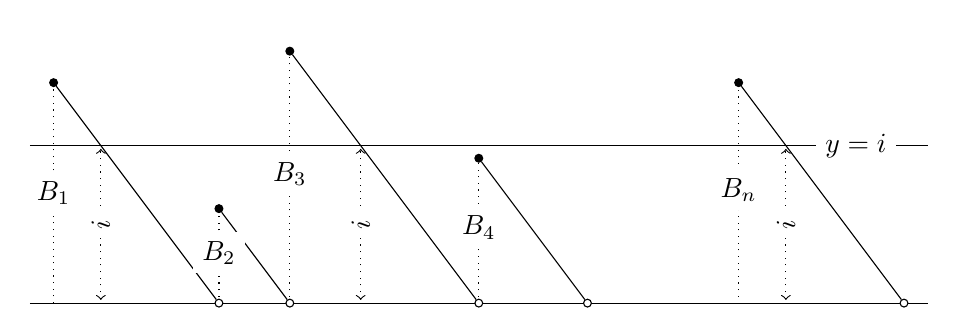
\begin{tikzpicture}[yscale=0.8,xscale=0.6,
 open/.style={shape=circle, fill=white, inner sep=1pt, draw, node contents=},
 closed/.style={shape=circle, fill=black, inner sep=1pt, draw, node contents=}]

 % y = zero line
 \draw (-0.5, 0) -- (18.5, 0); 
 % level crossing
 \draw (-0.5, 2.5) -- (18.5, 2.5) 
 %node[pos=0.65, fill=white, above] {$\sum_{k=1}^n \1{B_k \geq i}$}
 node[pos=0.92, fill=white] {$y=i$};


 \draw node (c1) at (0,3.5) [closed, label={}]
 node (c2) at (3.5,0)[open, label={}]
 (c1) to (c2);
 \draw[dotted] (0,0) -- (0,3.5) node[midway, fill=white] {$B_1$};
 \draw[dotted, <->] (1, 0.05) -- (1, 2.45) node[fill=white, midway, rotate=90] {$i$};


 \draw node (c1) at (3.5,1.5) [closed, label={}]
 node (c2) at (5,0)[open, label={}]
 (c1) to (c2);
 \draw[dotted] (3.5,0.1) -- (3.5,1.5) node[midway, fill=white] {$B_2$};

 \draw node (c1) at (5,4) [closed, label={}]
 node (c2) at (9,0)[open, label={}]
 (c1) to (c2);
 \draw[dotted] (5,0.1) -- (5,4) node[midway, fill=white] {$B_3$};
 \draw[dotted, <->] (6.5, 0.05) -- (6.5, 2.45) node[fill=white, midway, rotate=90] {$i$};

 \draw node (c1) at (9,2.3) [closed, label={}]
 node (c2) at (11.3,0)[open, label={}]
 (c1) to (c2);
 \draw[dotted] (9,0.1) -- (9,2.3) node[midway, fill=white] {$B_4$};

 % end
 \draw node (c1) at (14.5,3.5) [closed, label={}]
 node (c2) at (18,0)[open, label={}]
 (c1) to (c2);
 \draw[dotted] (14.5,0.1) -- (14.5,3.5) node[midway, fill=white ] {$B_n$};
 \draw[dotted, <->] (15.5, 0.05) -- (15.5, 2.45) node[fill=white, midway, rotate=90] {$i$};
 

 % bottom line
 %\draw[<->] (0, -0.6) -- (18, -.6) node[fill=white, midway] {$\sum_{k=1}^n B_k$};
\end{tikzpicture}

\caption{A batch crosses the line $y=i$ iff it contains at least $i$ items.
 Thus, during the service of a batch with $i$ or more items, there is precisely one service of an $i$-th item.}
 \label{fig:remainingservicetime}
\end{figure}


\begin{exercise}\clabel{ex:l-170}
 Now use the renewal reward theorem to show that the (time-average) fraction of time there are~$i$ items at the server is equal to
 \begin{equation*}
 \P{L_S = i} = \lambda \E{S} G(i-1) = \rho \frac{G(i-1)}{\E B}.
 \end{equation*}
Conclude that
\begin{equation*}
 \E{L_S} = \sum_{i=0}^\infty i \P{L_S=i} = \frac{\rho}{\E B} \sum_{i=1}^\infty i G(i-1).
\end{equation*}
\begin{solution}
 By construction, $Y_i(t)/t \to \P{L_S=i}$.
 Let $X_k = Y_i(D_k) - Y_i(D_{k-1})$.
 Then, since the $\{S_{k, i}\}$ are i.i.d. with $\E{S_{k,i}} = \E S$, 
 and the $\{B_k\}$ are i.i.d., we obtain from the previous exercise that $X = \lim_{n\to\infty} n^{-1}\sum_{k=1}^n (S_{k,i} \1{B_{k} \geq i}) = \E{S \1{B\geq i}}$.
 Now $B$ and $S$ are independent by assumption, hence $X = \E{S} \E{\1{B\geq i}} = \E S \P{B\geq i}$.
 The result follows by using rate stability ($\delta = \lambda$) in the renewal reward theorem.
\end{solution}
\end{exercise}



\begin{extra}\clabel{ex:ER}
 Show that
 \begin{equation*}
 \sum_{i=1}^\infty i G(i-1)= \frac{\E{B^2} + \E B}{2},
\end{equation*}
so that
\begin{equation*}
 \E{L_S} = \rho \frac{\E{B^2}}{2 \E B} + \frac{\rho}{2}.
\end{equation*}

\begin{hint}
 Use~\cref{ex:6} and~\cref{ex:66}.
\end{hint}
\begin{solution}
\begin{equation*}
 \begin{split}
 \sum_{i=1}^\infty i G(i-1) 
&=\sum_{i=0}^\infty (i+1) G(i) 
=\sum_{i=0}^\infty i G(i) +
\sum_{i=0}^\infty G(i)\\
&= (\E{B^2} - \E B + 2\E B)/2.
 \end{split}
\end{equation*}
\end{solution}
\end{extra}
  
\end{comment}


\opt{solutionfiles}{
\Closesolutionfile{hint}
\Closesolutionfile{ans}
\subsection*{Hints}
\input{hint}
\subsection*{Solutions}
\input{ans}
}

%\clearpage

%%% Local Variables:
%%% mode: latex
%%% TeX-master: "../companion"
%%% End:


\section{$M/G/1$ Queue: Expected Waiting Time}
%{$\mathbf{M/G/1}$ Queue: Expected Waiting Time}
\label{sec:mg1}



\opt{solutionfiles}{
\subsection*{Theory and Exercises}
\Opensolutionfile{hint}
\Opensolutionfile{ans}
}

In many practical single-server queueing systems the service times are not really well approximated by the exponential distribution.
The $M/G/1$ queue then becomes a better model than the $M/M/1$ queue.
In this section we first present a formula to compute the average waiting time in queue for the $M/G/1$ queue, and then we derive it by means of sample path arguments.
The derivation is also of general interest as it develops some general results of renewal theory.


The fundamentally important \recall{Pollaczek-Khinchine formula}, or \recall{PK formula}, for the average waiting time in queue for the $M/G/1$ queue has the form
\begin{equation} \label{eq:710}
% \E{W_Q} = \frac{\E{S_r}}{1-\rho} =\frac 1 2 \frac{\lambda \E{S^2}}{1-\rho} =\frac{1 + C_s^2}2 \frac{\rho}{1-\rho} \E S.
 \E{W_Q} = \frac{1 + C_s^2}2 \frac{\rho}{1-\rho} \E S.
\end{equation}
Before deriving this formula, let us apply it.

\begin{extra}
 Show that when services are exponential, the expected waiting time $\E{W_Q(M/G/1)}$ reduces to $\E{W_Q(M/M/1)}$.
\begin{solution}
 Since the SCV for the exponential distribution is $1$, hence
 $C_s^2=1$, we get 
 \begin{equation*}
\E{W_Q} = \frac{1+1}2\frac{\rho}{1-\rho} \E S = \frac{\rho}{1-\rho} \E S,
 \end{equation*}
which we also found in a previous section.
\end{solution}
\end{extra}


\begin{extra}
 Compute $\E{W_Q}$ and $\E L$ for the $M/D/1$ queue.
\begin{solution}
 For the $M/D/1$ the service time is deterministic.
 Thus, the service time $S=T$ always.
 Hence, $\E S = T$ and $\E{S^2}=T^2$, hence $\V S = \E{S^2} - (\E S)^2 = 0$, hence $C_s^2 = 0$.
 From the Pollaczek-Khinchine formula, the first term is $1+C_s^2=1$ for the $M/D/1$ queue, and $1+C_s^2=2$ for the $M/M/1$ queue.
 Hence,
 \begin{equation*}
\E{W_Q(M/D/1)} = \frac{\E{W_Q(M/M/1)}}2.
\end{equation*}
Therefore,
\begin{align*}
 \E{L(M/D/1)} &= \E{L_Q(M/D/1)} +\rho = \frac{\E{L_Q(M/M/1)}}2 + \rho \\
&= \frac{\rho^2}{2(1-\rho)} + \rho=\frac{\rho(2-\rho)} {2(1-\rho)}.
\end{align*}
\end{solution}
\end{extra}

\begin{extra}
 Compute $\E L$ for the $M/G/1$ queue with $S\sim U[0,\alpha]$.
\begin{hint}
Integrate $\alpha^{-1} \int_0^\alpha x \d x$, and likewise for the second moment.
\end{hint}
\begin{solution}
 \begin{align*}
\E S &= \alpha/2,\\
\E{S^2} &= \int_0^\alpha x^2 \d x/\alpha = \alpha^2/3\\
\V S &= \alpha^2/3 - \alpha^2/4= \alpha^2/12\\
C_s^2 &= (\alpha^2/12)/(\alpha^2/4) = 1/3,\\
\rho &= \lambda \alpha/2,\\
\E{W_Q} &= \frac{1+C_s^2}2 \frac{\lambda \alpha/2}{1-\lambda \alpha/2}\frac \alpha2, \\
\E W &= \E{W_Q} + \frac \alpha2,\\
\E L &= \lambda \E W.
 \end{align*}
\end{solution}
\end{extra}

\begin{exercise}\clabel{ex:l-240}
 A queueing system receives Poisson arrivals at the rate of 5 per hour.
 The single server has a uniform service time distribution, with a range of 4 minutes to 6 minutes.
 Determine $\E{L_Q}$, $\E L$, $\E{W_Q}$, $\E W$.
\begin{solution}
First the load.
\begin{pyconsole}
labda = 5./60 # arrivals per minute
a = 4.
b = 6.
ES = (a+b)/2. # service time in minutes
rho = labda*ES
rho
\end{pyconsole}

Next, the variance and SCV. With this the waiting times follow right away.
\begin{pyconsole}
Var = (b-a)*(b-a)/12.
SCV = Var/(ES**2)


Wq = (1+SCV)/2.*rho/(1.-rho)*ES
Wq # in minutes
Wq/60. # in hour


W = Wq + ES
W
Lq = labda*Wq
Lq
L = labda*W
L
\end{pyconsole}
\end{solution}
\end{exercise}



\begin{exercise}\clabel{ex:l-241}
 Consider a workstation with just one machine.
 We model the job arrival process as a Poisson process with rate $\lambda=3$ per day.
 The average service time $\E S = 2$ hours, $C^2_s = 1/2$, and the shop is open for 8 hours.
 What is $\E{W_Q}$?

 Suppose the expected waiting time has to be reduced to 1h.
 How to achieve this?
\begin{solution}
 $\E{W_Q} = 4.5$ h. $\rho = \lambda \E S = (3/8)\cdot 2 = 3/4$.

 One way to increase the capacity/reduce the average service time is to choose $\E S =1$ hour and reduce $C^2_s$ to $1/4$.
 Of course, there are many more ways.
 Reducing $C^2_S$ to zero is (nearly) impossible or very costly.
 Hence, $\rho$ must go down, i.e., capacity up or service time down.
 Another possibility is to plan the arrival of jobs, i.e., reduce the variability in the arrival process.
 However, typically this is not possible.
 For instance, would you accept this as a customer?
\end{solution}
\end{exercise}


\begin{exercise}[Hall 5.16] \clabel{ex:46}
The manager of a small firm would like to determine which of two people to hire.
 One employee is fast, on average, but somewhat inconsistent.
 The other is a bit slower, but very consistent.
 The first has a mean service time of $2$ minutes, with a standard deviation of 1 minute.
 The second has a mean service time of $2.1$ minutes, with a standard deviation of $0.1$ minutes.
 If the arrival rate is Poisson with rate 20 per hour, which employee would minimize $\E{L_Q}$?
 Which would minimize $\E L$?
\begin{solution}
 The arrival process is assumed to be Poisson. There is also
 just one server. Hence, we can use the PK formula to compute the average queue length.

\begin{pyconsole}
labda = 20./60 # per minute
ES = 2. # minutes
sigma = 1.
SCV = sigma*sigma/(ES*ES)
rho = labda*ES
rho

Wq = (1+SCV)/2 * rho/(1-rho) * ES
Wq
Lq = labda * Wq # Little's law
Lq
W = Wq + ES
W
L = labda * W
L
\end{pyconsole}


\begin{pyconsole}
ES = 2.1
SD = 0.1
SCV = SD**2/ES**2
rho = labda*ES
rho

Lq = rho**2/(1.-rho)*(1.+SCV)/2.
Lq
L = rho + Lq
L
\end{pyconsole}

\end{solution}
\end{exercise}


\begin{extra}
 Show that for the $M/G/1$ queue, the expected idle time is
 $\E I = 1/\lambda$. 
\begin{hint}
What is the average time between two
 arrivals? Observe that the inter-arrivals are memoryless, hence the
 average time until the next arrival after the server becomes idle
 is also $1/\lambda$.
\end{hint}
\begin{solution}
 Since the inter-arrival times are memoryless, the expected time to the first arrival after the system becomes empty is also $\E X=1/\lambda$.
\end{solution}
\end{extra}

\begin{extra}
 Express the utilization of the $M/G/1/1$ queue in terms of $\lambda$ and $\E S$.
\begin{solution}
 The system can contain at most 1 job.
 Necessarily, if the system contains a job, this job must be in service.
 All jobs that arrive while the server is busy are rejected.
 Just after a departure, the average time until the next arrival is $1/\lambda$, and then a new service starts with an average duration of $\E S$.
 After this departure, a new cycle starts.
 Thus, the utilization is $\E S/(1/\lambda + \E S) = \lambda \E S/ (1 + \lambda \E S)$.
 Since not all jobs are accepted, the utilization $\rho$ cannot be equal to $\lambda \E S$.
\end{solution}
\end{extra}

\begin{extra}
 For the $M/G/1/1$ queue what is the fraction of jobs rejected?
\begin{hint}
 The rate of accepted jobs is $\lambda \pi(0)$.
 What is the load of these jobs?
 Equate this to $1-\pi(0)$ as this must also be the load.
 Then solve for $\pi(0)$.
\end{hint}
\begin{solution}
 Let $p(0)$ be the fraction of time the server is idle. By PASTA,
 $\pi(0)=p(0)$. Thus, the rate of accepted jobs is
 $\lambda\pi(0)$. Therefore, the departure rate
 $\delta=\lambda\pi(0)$. The loss rate is
 $\lambda-\delta = \lambda (1-\pi(0))$.

 Since $\lambda\pi(0)$ is the rate at which jobs enter the system,
 the load must be $\lambda\pi(0)\E S$. Since the load is also
 $1-\pi(0)$, it follows from equating that
 \begin{equation*}
 \lambda\pi(0) \E S = 1 - \pi(0) \iff \pi(0)=\frac1{1+\lambda\E S} 
\iff 1-\pi(0) = \frac{\lambda \E S}{1+\lambda \E S},
 \end{equation*}
which is the same as in the previous problem.

Note that $\delta < \lambda$, as it should be the case. 
\end{solution}
\end{extra}


\begin{extra}
 Why is the fraction of lost jobs at a $M/G/1/1$ queue not necessarily the same as for a $G/G/1/1$ queue with the same load?
\begin{hint}
Provide an example.
\end{hint}
\begin{solution}
 Typically, in the $G/G/1$ queue, the arrivals do not see time-averages. Consequently, the fraction of arrivals that are blocked is not necessarily equal to the utilization~$\rho$.

 Again, take jobs with a duration 59 minutes and inter-arrival times of
 1 hour. The load is $59/60$, but no job is lost, also not in the
 $G/G/1/1$ case. Thus, $\delta=\lambda$ in this case.
\end{solution}
\end{extra}



To derive the PK-formula, suppose at first that we know the expected \recall{remaining service time} $\E{S_r}$, i.e., the expected time it takes to complete the job in service, if present, at the time a job arrives.




\begin{extra}\clabel{ex:32}
Show for the $M/G/1$ queue that the expected time in queue is
\begin{equation}\label{eq:24}
 \E{W_Q} = \E{S_r} + \E{L_Q} \E S.
\end{equation}
\begin{hint}
 What happens when you enter a queue? First you have to wait until the job in service (if there is any) completes, and then you have to wait for the queue to clear.
\end{hint}
\begin{solution}
It is evident that the expected waiting time for an arriving customer is the expected
remaining service time plus the expected time in queue. The expected
time in queue must be equal to the expected number of
customers in queue at an arrival epoch times the expected service time
per customer, assuming that service times are i.i.d. If the arrival
process is Poisson, it follows from PASTA that the average number of
jobs in queue perceived by arriving customers is also the
\emph{time-average} number of jobs in queue~$\E{L_Q}$. 
\end{solution}
\end{extra}


\begin{exercise}\clabel{ex:l-242}
Show that, given $\E{S_r}$, 
\begin{equation}\label{eq:35}
 \E{W_Q} = \frac{\E{S_r}}{1-\rho}.% = \frac{\rho}{1-\rho} \E{S_r\given S_r>0}.
\end{equation}
\begin{hint}
 Use~\cref{ex:32}. Then use Little's law to see that $\E{L_Q} = \lambda \E{W_Q}$. Substitute this in~\cref{eq:24} and simplify.
\end{hint}
\begin{solution}
With Little's law $\E{L_Q} = \lambda \E{W_Q}$. Using this,
\begin{equation*}
 \E{W_Q} = \E{S_r} + \lambda \E{W_Q} \E S =\E{S_r} + \rho \E{W_Q},
\end{equation*}
since $\rho=\lambda \E S$. But this gives for the $M/G/1$ queue that
\begin{equation*}
 \E{W_Q} = \frac{\E{S_r}}{1-\rho}.
\end{equation*}
\end{solution}
\end{exercise}



It remains to compute the average remaining service time $\E{S_r}$ for generally distributed service times.
Just like in~\cref{sec:mxm1-queue:-expected} we use the renewal reward theorem.
Consider the $k$th job of some sample path of the $M/G/1$ queueing process.
Let its service time start at time $\tilde A_k$ so that it departs at time $D_k=\tilde A_k + S_k$.

\begin{exercise}\clabel{ex:13}
 Use~\cref{fig:mg1remainingservicetime} to explain that the remaining service time of job $k$ at time $s$ is given by
\begin{equation*}
R_k(s) = (D_k-s)\1{\tilde A_k \leq s < D_k}.
\end{equation*}
With this, explain that
 \begin{equation*}
 Y(t) = \int_0^t (D_{D(s)+1}-s)\1{L(s) > 0} \d s
 \end{equation*}
is the total remaining service time as seen by the server up to $t$. 
\begin{solution}
 Observe that when $s\in [\tilde A_k, D_k)$, the remaining service time until job $k$ departs is $D_k-s $, while if $s\not \in [\tilde A_k, D_k)$, job $k$ is not in service so it cannot have any remaining service.

 At time $s$, the number of departures is $D(s)$.
 Thus, $D(s)+1$ is the first job to depart after time $s$.
 The departure time of this job is $D_{D(t)+1}$, hence the remaining service time at time $s$ is $D_{D(s)+1}-s$, provided this job is in service.
\end{solution}
\end{exercise}


\begin{figure}[htb]
 \centering
\begin{tikzpicture}[scale=1,
 open/.style={shape=circle, fill=white, inner sep=1pt, draw, node contents=},
 closed/.style={shape=circle, fill=black, inner sep=1pt, draw, node contents=}]
 \draw (-1,0) -- (4,0); 
 %x\draw (1,0) -- (3,0) node[midway, fill=white] {$s$};
 \draw node (c1) at (0,3) [closed, label={}]
 node (c2) at (3,0)[open, label={}]
 (c1) to (c2);
 \draw[dotted] (0,0) -- (0,3) node[midway, rotate=90, fill=white] {$S_k$};
 \node[below] at (0,0) {$\tilde A_k$};
 \node[below] at (3,0) {$D_k$};

 \draw[<->, dotted] (0.75,0) -- (0.75,2.25) node[midway,fill=white,rotate=90] {$D_k-s$};
 \node[below] at (0.75,0) {$s$};
 \end{tikzpicture}

 \caption{Remaining service time.}
 \label{fig:mg1remainingservicetime}
\end{figure}

\begin{exercise}\clabel{ex:l-243}
Apply the renewal reward theorem to the result of~\cref{ex:13} to prove that 
\begin{equation}\label{eq:34}
\E{S_r} = \frac{\lambda}2 \E{S^2}. 
\end{equation}
Then simplify to get~\cref{eq:710}. 
\begin{hint}
 Choose $T_k=D_k$ as epochs in the renewal reward theorem.
\end{hint}
\begin{solution}
 It is clear that the time-average $Y(t)/t \to \E{S_r}$.
 Moreover, $X_k = Y(D_k) - Y(D_{k-1})$ is the area under the triangle in~\cref{fig:mg1remainingservicetime}.
 Thus, $X=\lim_{n\to\infty} \lim_{k=1}^n S_k^2/ 2 = \E{S^2}/2$.
 Finally, $\delta = \lambda$ by rate-stability.

 The rest is plain algebra, see~\cref{ex:65}.
\end{solution}
\end{exercise}

\begin{extra}\clabel{ex:65}
Use $C_s^2 = \V S / (\E S)^2$ to show that $\lambda \E{S^2} = (1+C_s^2)\rho\E S$
\begin{solution}
Use that 
\begin{equation*}
 \frac{\E{S^2}}{(\E S)^2} = 
 \frac{(\E{S^2}-(\E S)^2) + (\E S)^2}{(\E S)^2} =
 \frac{\V S + (\E S)^2}{(\E S)^2} =
 C_s^2 + 1.
\end{equation*}
Then
\begin{equation*}
 \lambda\E{S^2} = \frac{\E{S^2}}{(\E S)^2} \lambda(\E S)^2=
 \frac{\E{S^2}}{(\E S)^2} \rho \E S = (1+C_s^2) \rho \E{S}.
\end{equation*}
\end{solution}
\end{extra}



\begin{extra}
Use the PASTA property to show that
\begin{equation}\label{eq:37}
\E{S_r} = \rho \E{S_r\given S_r>0}.
\end{equation}
\begin{hint}
 Use~\cref{ex:28}.
\end{hint}
\begin{solution}
By the PASTA property we know that $\rho$ is the probability to find the server busy upon arrival; hence $1- \rho$ is the probability that the server is idle upon arrival. Then,
\begin{equation*}
\E{S_r} = \rho \E{S_r\given S_r >0} + (1-\rho) \E{S_r\given S_r = 0} = \rho \E{S_r\given S_r>0},
\end{equation*}
since, evidently, $\E{S_r\given S_r=0}=0$. 
\end{solution}
\end{extra}

\begin{extra}
 It is an easy mistake to think that $\E{S_r} = \E S$ when service
 times are exponential. Why is this wrong?
\begin{hint}
Realize again that $\E{S_r}$ includes the jobs that arrive at an empty system.
\end{hint}
\begin{solution}

 $\E{S_r \given S_r>0} = \E S$ for the $M/M/1$ queue, and
 $\E{S_r} = \rho \E{S_r \given S_r>0}$ for the $M/G/1$ queue, it
 follows that
 \begin{equation*}
 \E{S_r} = \rho \E{S_r\given S_r>0} = \rho \E S.
 \end{equation*}
\end{solution}
\end{extra}




\begin{exercise} \clabel{ex:9}
Show from~\cref{eq:34} that 
\begin{equation}\label{eq:55}
\E{S_r\given S_r>0} = \frac{\E{S^2}}{2 \E S}.
\end{equation}
\begin{solution}
 From~\cref{eq:37} and the sentences above this equation,
 we have that
 \begin{equation*}
 \E{S_r} = \rho \E{S_r\given S_r>0}=\lambda \E S \E{S_r\given S_r>0}.
 \end{equation*}
Hence,
 \begin{equation*}
 \lambda \E{S_r\given S_r>0} = \frac{\E{S_r}}{\E S} = \lambda \frac{\E{S^2}}{2 \E S}.
 \end{equation*}
\end{solution}
\end{exercise}


\begin{extra}\clabel{ex:45}
\begin{equation*}
\E{S_r\given S_r>0} = \frac{\E{S^2}}{2 \E S} \implies \E {S_r\given S_r>0} = \frac{\E S} 2
\end{equation*}
when $\V{S} = 0$. 
\begin{hint}
 $\V S = 0$ implies that $S$ is deterministic.
\end{hint}
\begin{solution}
 When $S$ is deterministic $\E{S^2} = (\E{S})^2$. Now use~\cref{eq:55}.
\end{solution}
\end{extra}

\begin{extra}
 What is $\E{S_r\given S_r>0}$ for the $M/D/1$ queue? 
\begin{solution}
By~\cref{ex:45}, it is half the service time. 
\end{solution}
\end{extra}

\begin{extra}
Show that $\E{S_r\given S_r>0} = \alpha/3$ when $S \sim U[0, \alpha]$.
\begin{solution}
 When $S$ is uniform on $[0, \alpha]$,
 \begin{align*}
 \E S &= \alpha^{-1}\int_0^\alpha x \, \d x =\frac{\alpha^2}{2 \alpha} = \frac{\alpha}2, 
&
\E{S^2} &= \alpha^{-1}\int_0^\alpha x^2 \, \d x = \frac{\alpha^2}3. 
 \end{align*}
 Thus, with~\cref{eq:55}, $\E{S_r\given S_r>0} = (\alpha^2/3)/(2 \alpha/2) = \alpha/3$. 
\end{solution}
\end{extra}

\begin{extra}
 Show that $\E{S_r\given S_r>0} = \mu^{-1}$ when $S\sim \Exp(\mu)$.
\begin{solution}
 \begin{align*}
\E S &= \mu \int_0^\infty x e^{-\mu x}\,\d x = 1/\mu, \\
\E{S^2} 
&= \mu \int_0^\infty x^2 e^{- \mu x} \,\d x = - \left. x^2 e^{-\mu x} \right|_0^\infty + 2 \int_0^\infty x e^{-\mu x} \, \d x \\
&= -\left. 2\frac x \mu e^{-\mu x} \right|_0^\infty + \frac 2 \mu\int_0^\infty e^{-\mu x} \, \d x =\frac2{\mu^2}.
 \end{align*}
Now use~\cref{eq:55}.
\end{solution}
\end{extra}


\begin{extra}\clabel{ex:49}
 A machine serves two types of jobs.
 The processing time of jobs of type $i$, $i=1,2$, is exponentially distributed with parameter $\mu_i$.
 The type $T$ of a job is random and independent of anything else, and such that $\P{T=1} = p = 1-q = 1-\P{T=2}$.
 (An example is a desk serving men and women, both requiring different average service times, and $p$ is the probability that the customer in service is a man.)
 Show that the expected processing time and variance are given by
\begin{align*}
 \E S &= p \E{S_1} + q \E{S_2} \\
\V S &= p \V{S_1} + q \V{S_2} + pq(\E{S_1} - \E{S_2})^2.
 \end{align*}
Interestingly, we see that even if $\V{S_1} = \V{S_2} = 0$, $\V S > 0$
if $\E{S_1} \neq \E{S_2}$. Bear this in mind; we will use these ideas
later when we discuss the effects of failures on the variance of
service times of jobs.
\begin{hint}
 Let $S$ be the processing (or service) time at the server, and
 $S_i$ the service time of a type $i$ job. Then, 
 \begin{equation*}
 S = \1{T=1} S_1 + \1{T=2} S_2,
 \end{equation*}
 where $\1{\cdot}$ is the indicator function, that is, $\1{A}=1$ if the
 event $A$ is true, and $\1{A}=0$ if $A$ is not true. 
\end{hint}
\begin{solution}
With the hint, 
\begin{align*}
 \E S 
&= \E{\1{T=1} S_1} + \E{\1{T=2} S_2} \\
&= \E{\1{T=1}} \E{ S_1} + \E{\1{T=2}} \E{S_2}, \text{ by the independence of $T$}, \\
&= \P{T=1} /\mu_1 + \P{T=2}/ \mu_2 \\
&= p /\mu_1 + q/ \mu_2 \\
&= p \E{S_1} + q \E{S_2}.
\end{align*}
(The next derivation may seem a bit long, but the algebra is
standard. I include all steps so that you don't have to use pen and
paper yourself if you want to check the result.) Next, using that
\begin{equation*}
\1{T=1}\1{T=2} = 0 \text{ and } \1{T=1}^2 = \1{T=1},
\end{equation*}
we get
\begin{align*}
 \V S 
&= \E{S^2} - (\E S)^2 \\
&= \E{\left(\1{T=1} S_1 + \1{T=2} S_2\right)^2} - \left(\frac{p}{\mu_1}+\frac{q}{\mu_2}\right)^2 \\
&= \E{\1{T=1} S_1^2 + \1{T=2} S_2^2} - \left(\frac{p}{\mu_1}+\frac{q}{\mu_2}\right)^2 \\ 
&= p \E{S_1^2} + q \E{S_2^2} - \left(\frac{p}{\mu_1}+\frac{q}{\mu_2}\right)^2 \\ 
&= p \V{S_1} + p (\E{S_1})^2 + q \V{S_2} + q(\E{ S_2})^2 - \left(\frac{p}{\mu_1}+\frac{q}{\mu_2}\right)^2 \\ 
&= p \V{S_1} + \frac{p}{\mu_1^2} + q \V{S_2} + \frac{q}{\mu_2^2} - \left(\frac{p}{\mu_1}+\frac{q}{\mu_2}\right)^2 \\ 
&= p \V{S_1} + q \V{S_2}
+ \frac{p}{\mu_1^2} + \frac{q}{\mu_2^2}
- \frac{p^2}{\mu_1^2}-\frac{q^2}{\mu_2^2} -\frac{2pq}{\mu_1\mu_2}\\ 
&= p \V{S_1} + q \V{S_2}
+ \frac{p(1-p)}{\mu_1^2} + \frac{q(1-q)}{\mu_2^2}
-\frac{2pq}{\mu_1\mu_2}\\ 
&= p \V{S_1} + q \V{S_2}
+ \frac{pq}{\mu_1^2} + \frac{qp}{\mu_2^2}
-\frac{2pq}{\mu_1\mu_2}\\ 
&= p \V{S_1} + q \V{S_2}
+ pq(\E{S_1} - \E{S_2})^2.
\end{align*}
\end{solution}
\end{extra}



\opt{solutionfiles}{
\Closesolutionfile{hint}
\Closesolutionfile{ans}
\subsection*{Hints}
\input{hint}
\subsection*{Solutions}
\input{ans}
}

%\clearpage




%%% Local Variables:
%%% mode: latex
%%% TeX-master: "../companion"
%%% End:

\section{$M^X/M/1$ Queue Length Distribution}
%{$\mathbf{M^X/M/1}$ Queue Length Distribution}
\label{sec:batch-arrivals}




\opt{solutionfiles}{
\subsection*{Theory and Exercises}
\Opensolutionfile{hint}
\Opensolutionfile{ans}
}

In~\cref{sec:mxm1-queue:-expected,sec:mg1} we established the Pollaczek-Khinchine formula for the waiting times of the $M^X/M/1$ queue and the $M/G/1$ queue, respectively.
To compute more difficult performance measures, for instance the loss probability $\P{L>n}$, we need expressions for the stationary distribution $\pi(n)=\P{L=n}$ of the number of jobs in the system.
Here we present a numerical, recursive, scheme to compute these probabilities.

To find $\pi(n)$, $n=0, 1, \ldots$, we turn again to level-crossing arguments.
However, the reasoning that led to the level-crossing equation~\cref{eq:15} needs to be generalized.
To see this, we consider an example.
If $L(t)=3$, the system contains $3$ items.
(This is not necessarily the same as 3 batches.)
Since the server serves single items, down-crossings of level $n=3$ occur in single units.
However, due to the batch arrivals, when a job arrives it typically brings multiple items to the queue.
For instance, suppose that $L(A_k-) = 3$, i.e., job $k$ sees 3 items in the system at its arrival epoch.
If it's size $B_k = 20$, then right after the $k$th arrival the system contains 23 items, that is, $L(A_k)=3+20=23$.
Thus, upon the arrival of job $k$, all levels between states $3$ and $23$ are crossed.

The left panel in~\cref{fig:levelcrossing} shows all up- and down-crossings of some level $n$.
The down-crossing rate is easy: just as in~\cref{fig:A_n_t} there is just one arrow from right to left.
However, level~$n$ can be up-crossed from below from many states, in fact from any level $m, 0\leq m <n$.
More formally, to count the number of up-crossings define
\begin{equation*}
 A(m,n,t) = \sum_{k=1}^{A(t)}\1{L(A_k-) = m}\1{B_k > n-m}
\end{equation*}
as the number of jobs up to time $t$ that see $m$ in the system upon arrival and have batch size larger than $n-m$.
% With this, the total number of times level $n$ is up-crossed up to time~$t$ becomes
% \begin{equation*}
% A(n, t) = \sum_{m=0}^n A(m,n,t).
% \end{equation*}


% Observe that $\1{L(A_k-)\leq n}=1$ only when the $k$th job sees~$n$ or less items in the system, and $\1{L(A_k) > n}=1$ only after the $k$th arrival the system contains more than $n$ items.
% Thus, $\1{L(A_k-) \leq n}\1{ L(A_k)>n}=1$ iff the $k$th arrival generates an up-crossing of level~$n$.

% % Hence
% % \begin{equation*}
% % \sum_{k=1}^{A(t)} \1{L(A_k-) \leq n}\,\1{L(A_k)>n}
% % \end{equation*}
% % counts all up-crossings of level $n$ up to time $t$.


% From~\cref{fig:levelcrossing} we see that an up-crossing can be decomposed into:
% \begin{equation*}
% \begin{split}
% &\1{L(A_k-) \leq n}\1{L(A_k)>n} \\
% &= \1{L(A_k-) =n}\, \1{B_k >0} + \1{L(A_k-) =n-1}\1{ B_k >1} +\cdots + \1{L(A_k-) =0}\1{B_k > n} \\
% &= \sum_{m=0}^n \1{L(A_k-) =m}\1{B_k > n-m}.
% \end{split}
% \end{equation*}
% In other words, sample paths that up-cross level $n$ require that any job that
% sees $m$ ($m\leq n$) in the system upon arrival must bring a batch larger
% than $n-m$ items.



% As a consequence, it is not
% necessarily the case that $|A(n,t) - D(n,t)| \leq 1$ for all $t$, as
% was the case for queueing systems in which jobs arrive as single
% units. We need to generalize this inequality.

\begin{figure}[ht]
 \centering
\begin{tikzpicture}[scale=1,
 %Define standard arrow tip
 >=stealth',
 %Define style for boxes
 circ/.style={
 circle, 
 draw=black,
 thick,
 minimum size=1.cm,
 inner sep=0pt,
 text centered
 },
 % Define arrow style
 pil/.style={
 ->,
 thick,
 shorten <=2pt,
 shorten >=2pt}
]

\draw[dashed, thick] node at (5,-1.5) [below] {level $n$} 
(5,-1.5) -- (5,3);

\node[circ] (n-2) {$n-2$};

%\node[circ, right=of n-2] (n-1) {$n-1$} edge[loop below, thick] node[midway, fill=white] {$\lambda f(0)$} (n-1);
\node[circ, right=of n-2] (n-1) {$n-1$};

\node[circ, right=of n-1] (n) {$ n $}
 edge[pil,<-, bend left=45] node[below] {$\lambda f(1)$} (n-1.south east);
\node[circ, right=of n] (n+1) {$n+1$}
 edge[pil,bend left=45] node[midway, fill=white] {$\mu$} (n.south east);
\node[above=of n+1] (inf) {}
 edge[pil, <-, bend right=45] node[midway, fill=white] {$\lambda G(0)$} (n.north east)
 edge[pil, <-, bend right=45] node[midway, fill=white] {$\lambda G(1)$} (n-1.north east)
 edge[pil, <-, bend right=45] node[midway, fill=white] {$\lambda G(2)$} (n-2.north east)
;
\end{tikzpicture}
% \begin{tabular}
% \includegraphics[scale=0.9]{mxm1_2}
%&
% \includegraphics[scale=0.9]{mxm1_1}
% \end{tabular}
\caption{Level crossing of level $n$.
 Observe that when the system is in state $n-2$, the arrival of any batch larger than $2$ ensures that level $n$ is crossed from below.
 The rate at which such events happen is $\lambda \pi(n-2) G(2)$.
 Similarly, in state $n-1$ the arrival of any batch larger than one item ensures that level $n$ is crossed, and this occurs with rate $\lambda \pi(n-1) G(1)$, and so on.
}
 \label{fig:levelcrossing}
\end{figure}

\begin{extra}
 Show that $A(n, n,t) = A(n,t)$, where $A(n,t)$ is defined by~\cref{eq:19}.
\begin{solution}
 $A(n,n,t)$ counts all jobs up to time $t$ that see $n$ items
 and bring at least $n-n+1=1$ unit of work. As each job brings at
 least 1 item, $A(n,n,t)$ counts all jobs that see $n$ items at
 arrival.
\end{solution}
\end{extra}

\begin{exercise}\clabel{ex:70}
Assuming that the limits exist, show that
\begin{equation*}
\lim_{t\to\infty} \frac{A(m,n,t)}t = \lambda \pi(m) G(n-m).
\end{equation*}
\begin{solution}
For this purpose, observe that we can write
\begin{equation}\label{eq:16}
 \frac{A(m,n,t)}t = \frac{A(t)}t \frac{A(m,t)}{A(t)}\frac{A(m,n,t)}{A(m,t)}.
\end{equation}
By the assumptions of~\cref{sec:poisson-arrivals-see}, $A(t)/t\to\lambda$ and $A(m,t)/A(t)\to\pi(m)$.
Next, apply the results of~\cref{ex:68} to~\cref{ex:69}.
\end{solution}
\end{exercise}

\begin{extra}\clabel{ex:68}
Provided the limit exists, show that
\begin{equation}\label{eq:1332}
\lim_{t\to\infty} \frac{A(m,n,t)}{A(m,t)} =\P{B>n-m\given L(A-)=m},
\end{equation}
where the random variable $L(A-)$ denotes the number in the system seen by an arbitrary arrival.
\begin{solution}
\begin{equation*}
\lim_{t\to\infty} \frac{A(m,n,t)}{A(m,t)} = 
\lim_{t\to\infty} \frac{\sum_{k=1}^{A(t)}\1{L(A_k-) = m, B_k > n-m}}
{\sum_{k=1}^{A(t)}\1{L(A_k-) = m}}=\P{B>n-m\given L(A-)=m},
\end{equation*}
\end{solution}
\end{extra}


\begin{extra}\clabel{ex:69}
Show that $\P{B>n-m\given L(A-)=m}=\P{B>n-m}$.
\begin{hint}
 Realize that $B$ and $L(A-)$ are assumed to be independent.
\end{hint}
\begin{solution}
\begin{equation*}
 \begin{split}
\P{B>n-m\given L(A-)=m} &=
\frac{\P{B>n-m,L(A-)=m}}{\P{L(A-)=m}}\\
&=\frac{\P{B>n-m}\P{L(A-)=m}}{\P{L(A-)=m}} \\
&= \P{B>n-m} =G(n-m).
 \end{split}
\end{equation*}
\end{solution}
\end{extra}

Equating the number of up- and down-crossing gives $\sum_{m=0}^n A(m,n,t) \approx D(n,t)$. 
Then, dividing by~$t$, taking the limit $t\to\infty$, and using~\cref{ex:70} results in the level-crossing equation for the $M^X/M/1$ queue:
\begin{equation}\label{eq:42}
\lambda \sum_{m=0}^n \pi(m) G(n-m) = \mu \pi(n+1).
\end{equation}

\begin{exercise}\clabel{ex:l-153}
Provide an interpretation of~\cref{eq:42} in terms of a thinned Poisson arrival process.
\begin{solution}
 \Cref{eq:16} has the interpretation that the rate at which level $n$ is crossed from below from state $m$ is equal to the rate at which jobs arrive times the fraction of jobs that see $m$ jobs in the system times the fraction of jobs with batch size larger than $n-m$.
 Observe that the stream of jobs with batch size larger than $n-m$ is a Poisson process thinned at rate $G(n-m)$.
\end{solution}
\end{exercise}


\begin{extra}
 Show that~\cref{eq:42} reduces to $\mu \pi(n+1)=\lambda \pi(n)$ for the $M/M/1$ case.
\begin{solution}
 The right-hand side of~\cref{eq:42} is identical, so we only have to concentrate on the left-hand side.
 In the $M/M/1$ queue, all batches have size $1$.
 Thus, $\P{B=1} = f(1)=1$ and $f(k)=0$ for $k\neq 1$.
 Thus, $G(0)=1$ and $G(1)=G(2)=\cdots = 0$.
 Thus, $\sum_{m=0}^n G(n-m) \pi(m) = G(0)\pi(n)=\pi(n)$.
\end{solution}
\end{extra}



It is left to find the normalization constant.
As this recursion does not lead to a closed form expression for $\pi(n)$, such as~\cref{eq:23}, we need to use a criterion to stop this iterative procedure.
Finding general conditions when to stop is not directly easy, but a pragmatic approach is simple.
When the demand is finite, the numbers $\{\pi(k)\}$ should decrease geometrically fast when $k\geq N$ for some (large) $N$\footnote{An interesting question, why should it decrease monotonically after some, large, $N$?}.
Stop when $\pi(N)\ll \pi(0)$, and take $G=\sum_{i=0}^N \pi(i)$ as the normalization constant.
While this is a practical approach, getting formal bounds on a proper size of $N$ requires more work than we can do here.

Once again with $\pi(n)$ we can compute all performance measures we need, and study the influence on the batch size distribution and $\lambda$ and $\mu$ on the system's performance.

\begin{exercise}\clabel{ex:l-154}
 Why is~\cref{eq:39}, i.e., $\pi(n)=\delta(n)$, not true for the $M^X/M/1$ batch queue?
 Provide an example.
\begin{solution}
 Because arrivals do not occur in single units, but in batches.
\end{solution}
\end{exercise}

\begin{exercise}\clabel{ex:73}
 Substitute recursion~\cref{eq:42} for $\pi(n)$ into the expression $\E{L} = \sum_{n=0}^\infty n \pi(n)$ and derive~\cref{eq:43}.
\begin{solution}
 We chop this up into two steps, see~\cref{ex:71} and~\cref{ex:72}.
\end{solution}
\end{exercise}

\begin{extra}\clabel{ex:71}
 Step 1 of~\cref{ex:73}.
 Show that
\begin{equation}\label{eq:67}
 \mu \E L =\mu \sum_{n=0}^\infty n \pi(n) = \lambda \frac{\E{B^2}}2 + \lambda \E B \E L +\lambda \frac{\E B}2.
\end{equation}
\begin{hint}
 Substitute the recursion, and carry on with the algebra.
 Use also the results of the exercises of~\cref{sec:mxm1-queue:-expected}.
\end{hint}
\begin{solution}
 We use that $\mu \pi(n) =\lambda \sum_{i=0}^{n-1} \pi(i) G(n-1-i)$ and the results of the exercises of~\cref{sec:mxm1-queue:-expected} to see that
\begin{align*}
 \mu \E L
 &=\sum_{n=0}^\infty n\, \mu \pi(n), \quad \text{now substitute for $\mu \pi(n)$ the recursion~\cref{eq:42}}, \\
& =\lambda \sum_{n=0}^\infty n \sum_{i=0}^{n-1} \pi(i) G(n-1-i) 
 =\lambda \sum_{n=0}^\infty n \sum_{i=0}^\infty \1{i<n} \pi(i) G(n-1-i) \\
& =\lambda \sum_{i=0}^\infty \pi(i) \sum_{n=0}^\infty \1{i<n} n G(n-1-i) 
 =\lambda \sum_{i=0}^\infty \pi(i) \sum_{n=i+1}^\infty n G(n-1-i) \\
& =\lambda \sum_{i=0}^\infty \pi(i) \sum_{n=0}^\infty (n+i+1) G(n) 
 =\lambda \sum_{i=0}^\infty \pi(i) \left[\sum_{n=0}^\infty n G(n) +(i+1) \sum_{n=0}^\infty G(n)\right] \\
 &=\lambda \sum_{i=0}^\infty \pi(i)\sum_{n=0}^\infty n G(n) +\lambda \E B \sum_{i=0}^\infty \pi(i) (i+1) \\ 
 &=\lambda \sum_{i=0}^\infty \pi(i) \frac{\E{B^2} -\E B}2 + \lambda \E B (\E L +1) \\ 
 &= \lambda \frac{\E{B^2} -\E B}2 + \lambda \E B \E L +\lambda \E B \\
 &= \lambda \frac{\E{B^2} }2 + \lambda \E B \E L +\lambda \frac{\E B}2.
\end{align*}
\end{solution}
\end{extra}

\begin{extra}\clabel{ex:72}
 Step 2 of~\cref{ex:73}.
 Use~\cref{eq:67} and the definition $\rho=\lambda \E B/\mu$ to show that
\begin{equation*}
(1- \rho) \E L = \frac{\lambda}\mu \frac{\E{B^2}}2 + \frac\rho2.
\end{equation*}
\begin{solution}
 Dividing both sides of~\cref{eq:67} by $\mu$ and using that $\lambda \E B/\mu = \rho$,
\begin{equation*}
 \E L = \frac{\lambda}{\mu} \frac{\E{B^2}}2 + \rho \E L + \frac\rho2.
\end{equation*}
\end{solution}
\end{extra}



\begin{exercise}\clabel{ex:l-155}
 Implement the recursion~\cref{eq:42} in a computer program for the case $f(1)=f(2)=f(3)=1/3$.
 Take $\lambda =1$ and $\mu = 3$.
\begin{solution}
 The recursion for $n$ becomes
\begin{equation*}
\pi(n) = \frac \lambda \mu \sum_{i=0}^{n-1} \pi(n-1-i)G(i).
\end{equation*}
Since $G(i) =0$ for $i\geq 3$ we rewrite this to 
\begin{equation*}
 \pi(n) = \frac\lambda \mu \sum_{i=0}^{\min\{n-1,\text{len } G\}} \pi(n-1-i)G(i),
\end{equation*}
where $\text{len } G$ is the largest possible batch size.

The following code carries out the recursion for the $M/M/1$ queue and compares the result to the \emph{unnormalized} probabilities of the $M/M/1$ queue.
Recall, $(\lambda/\mu)^n$ are these unnormalized probabilities.
With this we can test the code right away.

\begin{pyconsole}
import numpy as np

f = [0, 1] # set f[0] = 0
F = np.cumsum(f) # distribution 
G = np.ones_like(F) - F # survivor function

labda = 1
mu = 3
num = 4
p = np.ones(num)

for n in range(1, num):
 p[n] = labda / mu * sum(p[n - 1 - i] * G[i] for i in range(min(n, len(G))))
 print(n, p[n], (labda / mu)**n)

\end{pyconsole}
The test is convincing. So now we'll move on the real problem. 

\begin{pyconsole}
f = np.ones(4) / 3
f[0] = 0
F = np.cumsum(f)
G = np.ones_like(F) - F
num = 30 # stop at 80
p = np.ones(num)
for n in range(1, num):
 p[n] = labda / mu * sum(p[n - 1 - i] * G[i] for i in range(min(n, len(G))))

p /= p.sum() # normalize
\end{pyconsole}

Now that we have the probabilities we can do all experiments we like. 
\begin{pyconsole}
EL = sum(n*p[n] for n in range(len(p)))
EL 
\end{pyconsole}

It is of interest to compare this result to~\cref{eq:43}.
In fact, I spent at least one hour to get~\cref{eq:43} correct; now I can finally check it numerically.


\begin{pyconsole}
EB = sum(k*fk for k,fk in enumerate(f))
rho=labda*EB/mu
EB2 = sum(k*k*fk for k,fk in enumerate(f))
VB = EB2 - EB*EB
C2 = VB/EB/EB
EL = (1+C2)/2*rho/(1-rho)*EB + rho/(1-rho)/2
EL
\end{pyconsole}

So, after all, stopping at 30 is not quite OK: there is a slight difference between the two expectations.
Let's run the recursion up to 100, and see what we get then.

\begin{pyconsole}
num = 100
p = np.ones(num)

for n in range(1, num):
 p[n] = labda / mu * sum(p[n - 1 - i] * G[i] for i in range(min(n, len(G))))

p /= p.sum() # normalize
EL = sum(n*p[n] for n in range(len(p)))
print(EL)
\end{pyconsole}
This does the job.
\end{solution}
\end{exercise}


We consider the $M^X/M/1/K$ queue, i.e., a batch queue in which at most $K$ jobs fit into the system.
When customers can be blocked in a batch queue it is necessary to specify a policy that decides which items in a batch to accept.
Three common rules are
\begin{enumerate}
\item Complete rejection: if a batch does not fit entirely into the system, it will be rejected completely.
\item Partial acceptance: accept whatever fits of a batch, and reject the rest.
\item Complete acceptance: accept all batches that arrive when the system contains $K$ or less jobs, and reject the entire batch otherwise.
\end{enumerate}

\begin{exercise}\clabel{ex:l-156}
 Derive a set of recursions, analogous to~\cref{eq:42}, to compute $\pi(n)$ for the $M^X/M/1/K$ queue with complete rejection.
\begin{solution}
 Suppose a batch of size $k$ arrives when the system contains $n$ jobs.
 When $k+n \leq K$, the batch can be accepted since the entire batch will fit into the queue.
 When, however, $k+n> K$, the batch has to be rejected.

 Now consider an imaginary line between states with $n$ and $n+1$ jobs in the system.
 This imaginary line separates the state space into two disjoint parts: one part with states $0, 1, \ldots, n$ and the other part with states $n+1, n+2, \ldots, K$.
 We call this imaginary line `level $n$'.
 We call an `up-crossing' a transition from some state $m\leq n$ to a state $l> n$.
 Likewise, a `down-crossing' of level~$n$ is a transition from some state $l> n$ to some state $m\leq n$.

 If the system contains $n$ jobs, level $n$ is crossed from below with rate $\lambda \pi(n) \P{B \leq K-n}$.
 More generally, when the system is in state $m\leq n$, we need a batch of at least $n+1-m$ to cross level~$n$.
 Moreover, any batch larger than $K-m$ gets rejected.
 Thus, when the system contains $m \leq n $ jobs, the rate at which level $n$ is crossed from below is
 \begin{equation*}
 \lambda \pi(m) \P{n+1-m\leq B \leq K-m} = \lambda \pi(m)
 [G(n-m)-G(K-m)],
 \end{equation*}
where we use that
\begin{align*}
\P{n+1-m\leq B \leq K-m} 
&= \P{B \leq K-m} - \P{B \leq n-m} \\
&= \P{B > n-m} - \P{B > K-m} \\
&= G(n-m)-G(K-m).
\end{align*}

 Since the server serves only single items, level $n$ can only be
 crossed from above from state $n+1$. This happens at rate $\mu p(n+1)$. With PASTA this is equal to $\mu \pi(n+1)$.

 Finally, since in the long run the number of up- and down-crossings must
 be the same, the up- and down-crossing rates must match. This implies
 that the balance equations becomes
 \begin{equation*}
 \mu \pi(n+1) = \lambda \sum_{m=0}^n \pi(m) [G(n-m)-G(K-m)],
 \end{equation*}
 for $n=0,\ldots, K-1$. 

 Before we continue with the other acceptance rules, it is important
 to check this result. In general, off-by-one errors are easily, and
 commonly, made, so we need to test the above on simple cases. 
 \begin{itemize}
 \item If $K\to \infty$, then $G(K-m)=\P{B>K-m}\to 0$, so we get our earlier result. 
 \item Take $n=K$. Then $G(n-m)-G(K-m)=0$ for all $m$. Then the right-hand side is 0, as it should.
 \item Taken $n=0$ and $K=1$, then $\mu \pi(1)= \lambda \pi(0)$. This also makes sense. 
 \item Take $n$ much smaller than $K$. If the batch size is maximally
 $2$, then for small $n$ the entire batch must fit. Let's see if
 this holds in the above formula. If $n$ much smaller than $K$,
 then also $m$ is much smaller than $K$ (since in the right-hand
 size, $m\leq n$). But then $G(K-m) \leq G(2) = 0$, as it
 should. (Observe that $G$ is a decreasing function of its argument;
 its a survival function.)
 \end{itemize}
\end{solution}
\end{exercise}


\begin{extra}
 Derive a set of recursions, analogous to~\cref{eq:42}, to compute $\pi(n)$ for the $M^X/M/1/K$ queue with complete acceptance.
\begin{solution}
 The complete-acceptance policy is actually quite simple. As any
 batch will be accepted when $n\leq K$, the queue length is not
 bounded. Only when the number of jobs in the system is larger than
 $K$, we do not accept jobs. 
 \begin{equation*}
 \mu \pi(n+1) = 
 \begin{cases}
 \lambda \sum_{m=0}^n \pi(m) G(n-m), & \text{ for } n\leq K,\\
 \lambda \sum_{m=0}^K \pi(m) G(n-m), & \text{ for } n> K.
 \end{cases}
 \end{equation*}
\end{solution}
\end{extra}

\begin{extra}
 Derive a set of recursions, analogous to~\cref{eq:42}, to compute $\pi(n)$ for the $M^X/M/1/K$ queue with partial acceptance.
\begin{solution}
 For the partial acceptance case, any job is accepted, but the system only admits whatever fits.
 As level $n\in {0,1,...,K-1}$ is still up-crossed by any batch of size at least $n-m$ when the system is in state $m$, the formula for the up-crossing rate is identical to the case without this acceptance policy.
 Moreover, nothing changes to the formula for the down-crossing rate.
 Hence,
 \begin{equation*}
 \mu \pi(n+1) = \lambda \sum_{m=0}^n \pi(m) G(n-m), 
 \end{equation*}
 for $n=0,1,\ldots, K-1$. 
\end{solution}
\end{extra}


\begin{extra}[Batch services, not obligatory]
 An interesting extension is a queueing process with batch services, i.e., the $M/M^Y/1$ queue.
 Constructing a recursion for the steady-state probabilities $\pi(n)$ for this case is not hard, in fact, mostly analogous to~\cref{eq:42}.
 However, solving the recursion appears to be quite a bit harder. 
\end{extra}



\opt{solutionfiles}{
\Closesolutionfile{hint}
\Closesolutionfile{ans}
\subsection*{Hints}
\input{hint}
\subsection*{Solutions}
\input{ans}
}

%\clearpage

%%% Local Variables:
%%% mode: latex
%%% TeX-master: "../companion"
%%% End:

\input{tex_files/mg1distributionqueuelength.tex}
% \input{tex_files/relationmxm1andmg1.tex}
%\input{tex_files/mg1density.tex}


\chapter{Queueing Control and Open Networks}
\label{cha:queu-contr-open}

TODO

In the queueing systems we analyzed up to now, the server is always present to serve jobs in the system. However, this condition is not always satisfied.
As an example, consider a queueing system in which there is a cost associated with switching on and off the server.
For instance, in some cases the server has to be set-up for operation; in other cases, the operator of a machine has to move from one place in the factory to another.
To reduce the cost, a so-called $N$-policy can be used, which works as follows, cf.~\cref{ex:n-policies}.
As soon as the system becomes empty (and the server idle), we switch off the server.
Then we wait until $N$ or more jobs arrived and then switch on the server.
The server processes jobs until the system is empty again, and then switches off again, and so on.
Thus, we use an $N$-policy to \emph{control} the queueing system, in particular the server, and the task is to find a switching threshold~$N$ that minimizes the long-run average cost.

Observe that under such policies the server occupancy can also increase.
In fact, this sometimes seems to the policy at dentists or hospitals: wait until the waiting room is quite full, and then start serving patients.
Like this the server minimizes idle time, and, in the example of a GP, the server (GP) does not have to wait for patients that might be late.

In this chapter we study the $M/M/1$ queue and $M/G/1$ under a $N$-policy, and then consider a $T$-policy.
We next focus on a policy that controls the server rate as a function of waiting time in the system.


We point out that the techniques developed in this chapter extend (way) beyond just queueing theory; they are worth memorizing.
Moreover, we illustrate many tools and results of the previous chapters.
Moreover, the concepts we introduce here can be generalized to (optimal) stopping problems, which find many applications beyond queueing, such in finance, inventory theory, decision theory, and so on.



\section{N-policies for the $M/M/1$ queue}
\label{sec:n-policies}


Let us consider the $M/M/1$ queue in which the server switches off as soon as it becomes idle and it costs~$K$ to switch on.
Supposing that each job charges $h$ Euros per unit time while in the system, it makes sense to build up a queue of jobs while the server is idle, and after some time switch on the server to process jobs until the system is empty again.
In particular, we analyze the influence of the $N$-policy on the long-run average cost.
For this we make a cost model in several steps and at the end we discuss how to minimize the cost as a function of the threshold~$N$.
In passing, we obtain a third way to compute the time-average number $\E L$ of jobs in the system; the first resulted from the analysis of the $M/M/1$ queue in~\cref{sec:mm1}, the second from Little's law, cf.~\cref{ex:l-215}

\opt{solutionfiles}{
\subsection*{Theory and Exercises}
\Opensolutionfile{hint}
\Opensolutionfile{ans}
}



Suppose the server is on, and there are $q$ jobs in the system.
Let us write $T(q)$ for the expected time to clear the system.
Now one of two events happens first.
Either a new job enters the system, or the job in service leaves.
It follows from~\cref{ex:3} that $\alpha=\lambda/(\lambda+\mu)$ is the probability the first event occurs and $\beta=\mu/(\lambda+\mu)$ is the probability the second occurs.
Moreover, from~\cref{ex:10} we see that the expected time to either an arrival or a departure, whichever is first, is $1/(\mu+\lambda)$.
Therefore, $T(q)$ must satisfy the following recursion:
\begin{equation}
  \label{eq:92}
  T(q) = \alpha T(q+1) + \beta T(q-1) + \frac{1}{\lambda+\mu}. 
\end{equation}
The reader should note that this type of recursion is a difference equation.
Moreover, the ideas behind its derivation are very similar to the ideas used in dynamic programming.

\begin{exercise}\clabel{ex:aab}
Provide an intuitive explanation for this formula, and show that $T(q)=q/(\mu-\lambda)$ solves~\cref{eq:92}. 
\begin{hint}
We just guess the form $T(q) = aq + b$, i.e., linear in $q$. It is clear that $T(0)=0$: if the system is empty, the time to clear it is zero. Thus, $b=0$, and it remains to solve for $a$. 
\end{hint}

\begin{solution}
  Jobs come in at rate $\lambda$ and are served at rate $\mu$.
  Therefore the systems drains at rate $\mu-\lambda$.
  When there are $q$ jobs in the system, it must take $q/(\mu-\lambda)$ units of time to serve these jobs.

  We substitute the guess $T(q) = aq$ in ~\cref{eq:92}, and solve for $a$. Specifically,
  \begin{equation*}
    a q = \alpha (aq + a) + \beta (a q - a) + 1/(\lambda+\mu). 
  \end{equation*}
Noticing that $\alpha + \beta = 1$, this reduces to $0 = a(\alpha - \beta) + 1/(\lambda + \mu)$. The rest is trivial.
\end{solution}
\end{exercise}


With the same line of reasoning we can compute the expected cost $V(q)$ to clear the system.
Noting that the queueing cost is $hq$ per unit time when there are $q$ jobs in the system, $V(q)$ must satisfy the relation
\begin{equation}\label{eq:93}
  V(q) = \alpha V(q+1) + \beta V(q-1) + h\frac{q}{\lambda + \mu}.
\end{equation}
%because $1/(\lambda + \mu)$ is the expected time we have to wait until either an arrival or a departure occurs.


To solve this, observe that in~\cref{eq:92} the last term is a constant, and that $T(q)$ is a linear function in~$q$.
In the recursion for $V(q)$ we see that the last term is linear in $q$ which leads us to the guess $a q^2 + b q + c$ for $V(q)$.
Thus, we substitute this into the above expression and then try to solve for $a,b$ and $c$.\footnote{The reader might wonder about the uniqueness of the solution.
  Noting that $V(q+1)$ follows directly from $V(q)$ and $V(q-1)$, there can be just one solution.}
As $V(0)=0$, it follows already that $c=0$.
Thus, it remains to find $a$ and $b$.

\begin{exercise}\clabel{ex:nmm-2}
  Use the ideas of~\cref{ex:aab} to show that
  \begin{equation*}
    V(q) = a q^2 + b q = \frac h 2 \frac 1 {\mu -\lambda} q^2 + \frac h 2 \frac{\lambda + \mu}{(\mu - \lambda)^2}q.
  \end{equation*}

\begin{hint}
  Fill in our guess $V(q) = aq^2 + bq$ in the recursion~\cref{eq:93}.
  Then, match the coefficients of $q^2$, $q$ and the constants, and use that $\alpha + \beta = 1$.
\end{hint}

\begin{solution}
 Filling our guess $V(q) = aq^2 + bq$ in the recursion~\cref{eq:93}  gives
  \begin{equation*}
    aq^2 + b q = \alpha a (q^2 + 2q + 1) + \alpha b (q+1) + \beta a (q^2 - 2q + 1) + \beta b (q - 1) + hq/(\lambda + \mu). 
  \end{equation*}
  Matching the coefficients of $q^2$, $q$ and the constants, and using that $\alpha + \beta = 1$, we obtain
  \begin{align*}
    a &= \alpha a + \beta a &\implies a &= a, \\
    b &= \alpha a 2 + \alpha b - \beta a 2 + \beta b + h/(\lambda + \mu), & \implies a &= \frac h 2 \frac 1 {\mu -\lambda},\\
    0 &= \alpha a + \alpha b + \beta a - \beta b, & \implies b &= \frac a {\beta - \alpha}. 
  \end{align*}
By combining the last two equations we get the answer. 
\end{solution}
\end{exercise}


Interestingly, the above turns out to be immediately useful.
Suppose we switch on the server when $N=1$, that is, directly at the arrival of the first job after the system became empty.
Write $C(1)$ for the expected duration of a cycle that starts when the system becomes idle and stops when the system becomes idle again (and after at least one job has arrived).
In other words, the cycle consists of an idle and a busy period.

\begin{exercise}\clabel{ex:nmm-3}
Explain that $C(1)=1/\lambda + T(1)$ for the $M/M/1$ queue.
\begin{hint}
  What is the expected  time to a job just after the server becomes idle? (Use the memoryless property.)
\end{hint}
\begin{solution}
  After clearing the system, we have to wait for a new job.
  The expected time for this job arrival is $1/\lambda$.
  (How do we use the memoryless property here?)
  Once the job arrived, the busy period starts with this one job, and the expected busy time is $T(1)$.
\end{solution}
\end{exercise}

\begin{exercise}\clabel{ex:nmm5}
Use the renewal-reward theorem to explain the  relation
\begin{equation*}
  \frac{V(1)}{C(1)} = \frac{V(1)}{1/\lambda + T(1)} = h \E L,
\end{equation*}
where $\E L$ is given by~\cref{eq:el}. Then use the above expressions for $V(1)$ and $C(1)$ to verify this.

With this result, we have found yet another way to compute the expected number of jobs in the system.  
\begin{hint}
  What is the cost of one cycle? What is the duration of one cycle? 
\end{hint}
\begin{solution}
  First the explanation.
  On the one hand, the cost of the jobs in the system during one cycle must be $V(1)$.
  The duration of one cycle is $C(1)$.
  By the renewal-reward theorem, the time-average cost must then by $V(1)/C(1)$.
  On the other hand, if the time-average number of jobs in the system is $\E L$, and each job pays $h$ per unit time, the time-average cost must be $h \E L$.

  Now the check; it's plain algebra:
\begin{align*}
  \frac{V(1)}{1/\lambda + T(1)}
  &= \frac{a+b}{1/\lambda + 1/(\mu-\lambda)} \\
  &= \left(\frac h 2 \frac 1 {\mu -\lambda} + \frac h 2 \frac{\lambda + \mu}{(\mu - \lambda)^2}\right)\frac{\lambda(\mu-\lambda)}{\mu}\\
&=\frac{h}2 \rho \left(1 + \frac{\lambda+\mu}{\mu-\lambda}\right) = \frac{h}{2} \rho \frac{2\mu}{\mu-\lambda}  \\
&= h \frac{\rho}{1-\rho} = h \E L. \\
\end{align*}
\end{solution}
\end{exercise}

It remains to generalize to a general threshold $N$; just above we already covered the case with $N=1$.
As we already have expressions for the cost and time for the time the server is on, we only have to consider the cost and time while the server is off.
Note that right after the server switches off, we need $N$ independent inter-arrival times to reach level $N$.
By~\cref{ex:54}, the expected time  to switch on must be equal to $N/\lambda$.

For the cost while building up the queue, we use again a recursive procedure.
Write $W(q)$ for the accumulated queueing cost from the moment the server becomes idle up to the arrival time of the $q$th job (the job that sees $q-1$ jobs in the system).
Then, by the next exercise,
\begin{equation}\label{eq:99}
  W(q) = W(q-1) + h\frac{q-1}{\lambda} = h \frac{q(q-1)}{2\lambda}.
\end{equation}

\begin{exercise}\clabel{ex:nmm-4}
Explain the above recursion, and derive the right-hand side.
\begin{hint}
  Use~\cref{eq:61}.
\end{hint}
\begin{solution}
  The cost up to the $q$th job is the cost up to the arrival of job $q-1$ plus the cost while there are $q-1$ jobs in the system.
  The time between the arrival of job $q-1$ and $q$ is $1/\lambda$.

  It is clear that $W(0)=0$. Therefore, $W(q) = h\sum_{i=1}^q (i-1) = hq(q-1)/2\lambda$. 
\end{solution}
\end{exercise}

It remains to assemble all results. Let us assume that the switching cost is $K$. Then, by the renewal-reward theorem, the time-average cost of the $N$-policy is equal to
\begin{equation*}
  \frac{W(N)+K+V(N)}{C(N)},
\end{equation*}
where $C(N) = N/\lambda + T(N)$.

Finding the optimal $N$ is easy (from a practical point).
Observe that $V(N)$ and $W(N)$ are quadratic in $N$, while $C(N)$ is linear in $N$.
Hence, the average cost is a convex function of $N$, and locating the minimizer of a one-dimensional convex function is simple.



\opt{solutionfiles}{
\Closesolutionfile{hint}
\Closesolutionfile{ans}
\subsection*{Hints}
\input{hint}
\subsection*{Solutions}
\input{ans}
}

%\clearpage 


%%% Local Variables:
%%% mode: latex
%%% TeX-master: "../companion"
%%% End:

\section{N-policies for the $M/G/1$ queue}
\label{sec:n-policies-mg1}

Interestingly, we can extend the analysis of~\cref{sec:distr-queue-length} and~\cref{sec:n-policies} to compute the average cost of the $M/G/1$ queue under an $N$-policy.
Thus, rather than exponentially distributed service times, we now consider general service times.
For the rest, the model and the problem is the same as in~\cref{sec:n-policies}. 

\opt{solutionfiles}{
\subsection*{Theory and Exercises}
\Opensolutionfile{hint}
\Opensolutionfile{ans}
}


Similar to~\cref{sec:distr-queue-length}, we consider the $M/G/1$ queueing process at departure moments.
It is easy to find an expression for the time to clear the queue right after the departure of a job that leaves $q$ jobs behind.
Analogous to~\cref{eq:92} and using the definition of $f(k)=\P{Y=k}$ as the probability that $Y=k$ jobs arrive during an arbitrary service time, we see that $T(q)$ must satisfy the relation
\begin{equation*}
  T(q) = \sum_{k=0}^\infty f(k) T(q+k-1) + \E S.
\end{equation*}
To see this, observe that when $k=0$ the next level is $q-1$ so that it takes $T(q-1)$ time to hit level~$0$.
When $k=1$, the level returns to $q$ after the departure of the job currently in service; consequently, we have not made any progress, hence we still need $T(q)$ units of time,  and so on.
Similar to the reasoning in~\cref{sec:n-policies}, we guess that $T(q) = a q + b$. Since $T(0)=0$, we already have $b=0$. 

\begin{exercise}\clabel{ex:nmg3}
Substitute $T(q) = a q$ in the above recursion for $T(q)$, and solve for $a$ to obtain
\begin{equation*}
  T(q) = \frac{\E S}{1- \E Y}q = \frac{\E S}{1-\lambda \E S}q.
\end{equation*}
\begin{hint}
  Use that $\sum_{k=0}^\infty k f(k) = \E Y$. Then use~\cref{ex:mg1-3}. Realize also that $\sum_k f(k) = 1$. 
\end{hint}
\begin{solution}
  \begin{align*}
    a q = \sum_{k=0}^\infty a (q+k-1) f(k) + \E S \implies a q = a q + a \E Y - a + \E S.
  \end{align*}
The terms linear in $q$ cancel. And thus, $0=a\E Y - a + \E S$. The result follows right away.
\end{solution}
\end{exercise}

Let $V(q)$ be the cost to clear the system right after a departure that leaves $q$ jobs behind.
Thus, $V(0)=0$.
Again, analogous~\cref{sec:distr-queue-length} and the derivation above for $T(q)$, we see that $V(q)$ must satisfy the relation
\begin{equation}
  \label{eq:98}
  V(q) = \sum_{k=0}^\infty f(k) V(q+k-1) + H(q), 
\end{equation}
where $H(q)$ is the queueing, or holding, cost, which we will determine next.

The queueing cost $H(q)$ consists of two components.
The first is the cost to keep $q$ jobs in the system while there is a job in service.
Clearly, the expected cost of this is $h q \E S$.
The second component is the cost of new jobs that arrive during the service.
While this is slightly harder to determine, we can combine the ideas underlying the derivation in~\cref{eq:99} the results of \cref{ex:35} to \cref{ex:p-35}.
Specifically, assume it is given that the service time is~$s$.
Then the average queueing cost $U(s)$ of the new arrivals must satisfy for some $0<\delta\ll 1$
\begin{equation*}
  U(s) = U(s-\delta) + (1-\lambda \delta)\cdot 0 + \lambda \delta h s + o(\delta).
\end{equation*}
This follows because during the interval $[0,\delta]$ a job arrives with probability $\lambda \delta$ and this stays $s$ time units in the system, while with probability $1-\lambda \delta$ no job arrives, and the cost of this is~$0$.
By the next problem, 
\begin{equation*}
  U(s) = \lambda h \frac{s^2}2. 
\end{equation*}

\begin{exercise}\clabel{ex:nmg4}
Assuming that $U(\cdot)$ is differentiable, we can use that $(U(s) - U(s-\delta))/\delta \approx U'(s)$.
Use this in the above to arrive at the differential equation $U'(s) = \lambda h s$ that $U$ must satisfy with condition $U(0)=0$ (why is this so?).
Solve this DE to conclude that $U(s)$ is as given above. 
\begin{solution}
Is it plain algebra:
\begin{align*}
  U(s)&=  U(s-\delta) + (1-\lambda \delta)\cdot 0 + \lambda \delta h s + o(\delta) &\implies\\
  (U(s) -U(s-\delta))/\delta &= \lambda h s + o(\delta) & \implies \\
  U'(s)&= \lambda h s, \quad\text{as } \delta \to 0.
\end{align*}
Integrating  both sides with respect to $s$ gives $U(s) - U(0) = \lambda h s^2/2$. As $U(0)=0$, we obtain the final result.
\end{solution}
\end{exercise}

Since $U(s)$ is the expected cost given that the service time is $s$, it follows from~\cref{ex:mg1-3} that $\E{U(S)} = \lambda h \E{S^2}$ is the expected queueing cost of the new jobs that arrive during the service. By combining the first and second component of $H(q)$, we obtain
\begin{equation*}
  H(q) = h q \E S + \frac 12 \lambda h \E{S^2}.
\end{equation*}
To solve~\cref{eq:98}, note that as in~\cref{eq:93}, the cost $H(q)$ has a term linear in~$q$ and a constant term.
Thus, once again, we guess that $V(q)$ is a quadratic function in $q$.
Then we substitute this form into~\cref{eq:98}, assemble terms with the same power in $q$, and try to solve for the coefficients in $aq^2 + bq+c$.
If we succeed, the solution we found must be correct, as a difference equation of the type~\cref{eq:98} can have just one solution once the boundary conditions are given.
Again, $V(q)=0 \implies c = 0$.
In fact, observe that we have all elements to compute the costs; except for (quite a bit of) algebra, we are done!

\begin{extra}
Assemble all terms of $V(q) = \sum_k V(q+k-1) + H(q)$ by their power in $q$ to obtain:
\begin{align*}
  a q^2 &= a q^2, \\
  b q &= 2a q \E Y - 2a q + b q + h q \E S,\\
  0 &= a \E{Y^2} - 2a \E Y + a + b \E Y - b + \frac 12 \lambda h \E{S^2}.
\end{align*}
\begin{hint}
  Just expand the left- and right-hand sides, and equate the terms with the same power in $q$.
\end{hint}
\begin{solution}
  Just expand
  \begin{equation*}
    \sum_{k=0}^\infty f(k)[ a(q+k-1)^2 + b(q+k-1)] + H(q),
  \end{equation*}
  and use that $\sum_k f(k) k = \E Y$ and $\sum_k f(k) k^2 = \E{Y^2}$. 
\end{solution}
\end{extra}

\begin{extra}
Simplify the above to obtain
\begin{align*}
  a &= \frac{h \E S}{2(1-\E Y)}, \\
  b(1-\E Y) &= a(\E{Y^2} - 2 \E Y + 1) + \frac 12 h \lambda \E{S^2}.
\end{align*}
\begin{solution}
  The first equation in the previous equation is superfluous.
  In the second we can cancel $bq$ at both sides.
  Simplifying gives us the expression for $a$.
  Similar for the third equation.
\end{solution}
\end{extra}

\begin{extra}
  Show that $\E{Y^2} = \lambda^2 \E{S^2} + \lambda \E S$. 
\begin{solution}
This follows directly from~\cref{ex:mg1-3}.
\end{solution}
\end{extra}

\begin{exercise}\clabel{ex:nm-2}
Show that 
\begin{align*}
  a &= \frac{h \E S}{2(1-\rho)}, &
  b &= \frac{h \E S}{2(1-\rho)^2} \left( 1+ \rho C_s^2\right).
\end{align*}
(In a sense, this is trivial, as it is just algebra, but it is hard to get the details right.)
\begin{solution}
  We already derived $a$, except that we replaced $1-\E Y= 1-\lambda \E S = 1-\rho$. 
For $b$, and using the expressions for $\E Y$ and $\E{Y^2}$, 
\begin{align*}
b(1-\E Y) &= a(\E{Y^2} - 2 \E Y + 1) + \frac 12 h \lambda \E{S^2} \\
&= \frac{h \E S}{2(1-\E Y)} (\E{Y^2} - 2 \E Y + 1) + \frac 12 h \lambda \E{S^2} \\
&= \frac{h \E S}{2(1-\lambda \E S)} \left(\lambda^2 \E{S^2} + \lambda \E S - 2 \lambda \E S + 1 +  \lambda \E{S^2}\frac{1-\lambda \E S}{\E S}\right) \\
&= \frac{h \E S}{2(1-\lambda \E S)} \left(\lambda^2 \E{S^2} - \lambda \E S + 1 +  \frac{\lambda \E{S^2}}{\E S} - \lambda^2 \E{S^2}\right) \\
&= \frac{h \E S}{2(1-\lambda \E S)} \left(1+ \frac{\lambda \E{S^2}}{\E S }  - \lambda \E S \right) \\
&= \frac{h \E S}{2(1-\lambda \E S)} \left( 1+ \frac{\lambda \E{S^2}}{\E S }  - \lambda \frac{(\E S)^2}{\E S}\right) \\
&= \frac{h \E S}{2(1-\lambda \E S)} \left( 1+ \lambda \frac{\V{S}}{\E S }\right)\\
&= \frac{h \E S}{2(1-\lambda \E S)} \left( 1+ \lambda \frac{\V{S}}{(\E S)^2 } \E S\right)\\
&= \frac{h \E S}{2(1-\lambda \E S)} \left( 1+ \rho C_s^2\right).
\end{align*}
Divide now both sides by $1-\E Y$. 
\end{solution}
\end{exercise}

\begin{extra}
We need to check our work.  For this reason, show that the results of~\cref{ex:nm-2} reduce to those of~\cref{ex:nmm-2} for the $M/M/1$ queue. 
\begin{solution}
  For $a$, multiply the numerator and denominator by $\mu=1/ \E S$.
  For $b$, multiply by $\mu^2 = 1/(\E S)^2$, use that $C_s^1=1$ because the service times are exponentially distributed, and note that
  \begin{equation*}
    \frac{1+\rho}{1-\rho} = \frac{\mu + \lambda}{\mu-\lambda}.
  \end{equation*}
\end{solution}
\end{extra}

\begin{exercise}\clabel{ex:nmg5}
As in~\cref{sec:n-policies}, show that we can obtain the Pollaczek-Khinchine equation~\cref{eq:710} with the results we have obtained up to now. 
\begin{hint}
  What is the cycle time $C(1)$ when the service starts with one job in the system? 
\end{hint}
\begin{solution}
  Right after the arrival of the first job that sees an empty system, the service of this job starts.
  Thus, $C(1) = 1/\lambda + T(1)$ is the expected duration of a cycle, and $V(1)$ the expected queueing cost of once cycle.
  The rest is algebra:
  \begin{align*}
    \frac{V(1)}{1/\lambda + T(1)}
    &= \frac{a + b}{1/\lambda + \E S/(1-\lambda \E S)} \\
    &= \frac{h} 2 \frac{\E S}{1-\rho} \frac{1 + (1+\rho C_s^2 )/(1-\rho)}{1/\lambda + \E S /(1-\rho)} \\
    &= \frac{h} 2 \frac{\E S}{1-\rho} \frac{1-\rho + 1 +\rho C_s^2}{(1-\rho)/\lambda + \E S} \\
    &= \frac{h} 2 \frac{\E S}{1-\rho} \frac{1-\rho + 1 +\rho C_s^2}{1/\lambda } \\
    &= \frac{h} 2 \frac{\rho}{1-\rho} (1-\rho + 1 +\rho C_s^2) \\
    &= \frac{h} 2 \frac{\rho}{1-\rho} (2-2\rho + \rho +\rho C_s^2) \\
    &= h \rho + \frac h 2 \frac{\rho^2}{1-\rho} (1+ C_s^2).
  \end{align*}
It checks!  
\end{solution}
\end{exercise}

For the $M/G/1$ queue it is evident that the expected queueing cost while the server is idle is also given by~\cref{eq:99}.
With this, and noting that there is a cost~$K$ to switch on the server, it follows from~\cref{ex:n-mg3} that the long-run time-average average costs are equal to
\begin{equation}
  \label{eq:100}
    \frac{V(N) + K + W(N)}{C(N)}
    = \frac h 2 \frac{\rho^2}{1-\rho} (1+ C_s^2) + h \rho + h \frac{N-1}2 + K \frac{\lambda(1-\rho)}N.
\end{equation}
Note that, if $N=1$ and $K=0$, this reduces to $h \E L$, as it should by our work above.
Finally, minimizing over $N$ gives that
\begin{equation*}
  N^* \approx \sqrt{\frac{2\lambda(1-\rho)K}{h}}.
\end{equation*}

\begin{remark}
  The expression for $N^*$ is a famous result in inventory theory: it is the optimal order size for a machine that produces items with holding cost $h$ per item per unit time, a cost $K$ to switch on the machine, demand arrives at rate $\lambda$, and the machine produces at rate $\mu=1/\E S$.
  $N^*$ is known as the \recall{Economic Production Quantity (EPQ)}.
  Taking $\mu\to\infty$, it reduces to the \recall{Economic Order Quantity (EPQ)}.
\end{remark}

\begin{exercise}\clabel{ex:n-mg3}
Derive~\cref{eq:100}.
\begin{solution}
  Note first that $C(N) = N(1/\lambda + \E S / (1-\rho)) = N/(\lambda(1-\rho))$. Then,
  \begin{align*}
    \frac{V(N) + K + W(N)}{C(N)}
    &= \left(aN^2 + bN + K + h N(N-1)/2 \lambda\right) \frac{\lambda(1-\rho)}N \\
    &= \frac h 2 \rho N  + \frac h 2 \frac \rho{1-\rho} (1+\rho C_s^2) + \frac h 2 (N-1)(1-\rho) + K \frac{\lambda(1-\rho)}N \\
    &= \frac h 2 \frac \rho{1-\rho} (1+\rho C_s^2) + \frac h 2 (N-1 + \rho) + K \frac{\lambda(1-\rho)}N \\
    &= \frac h 2 \frac \rho{1-\rho} (\rho + \rho C_s^2 + 1 - \rho) + \frac h 2 (N-1 + \rho) + K \frac{\lambda(1-\rho)}N \\
    &= \frac h 2 \frac{\rho^2}{1-\rho} (1+ C_s^2) +\frac h 2 \rho + \frac h 2 (N-1 + \rho) + K \frac{\lambda(1-\rho)}N \\
    &= \frac h 2 \frac{\rho^2}{1-\rho} (1+ C_s^2) + h \rho + h \frac{N-1}2 + K \frac{\lambda(1-\rho)}N.
  \end{align*}
%With the above expressions for $a$ and $b$ the result follows immediately. 
\end{solution}
\end{exercise}


\opt{solutionfiles}{
\Closesolutionfile{hint}
\Closesolutionfile{ans}
\subsection*{Hints}
\input{hint}
\subsection*{Solutions}
\input{ans}
}

%\clearpage 


%%% Local Variables:
%%% mode: latex
%%% TeX-master: "../companion"
%%% End:

\section{Open Single-Class Product-Form Networks}
\label{sec:jackson-networks}


Up to now our analysis focused on single-station queueing systems.
In many practical situations, however, jobs in a factory or patients in a hospital have to undergo several process steps before they are `finished'.
One of the simplest models to analyze such situations is to assume that jobs arrive as a Poisson processes, and the service times are exponentially distributed.
We will see that it is possible to obtain closed-form expressions for the stationary distribution of jobs at each station.
To establish this we will first concentrate on two stations in tandem, and then extend to general networks.
We remark that in~\cref{sec:tandem-queues} we considered tandem networks of $G/G/c$ queues, but there we could only obtain insight in the expected times, not the full distribution of the number of jobs at each station.

\subsection*{Theory and Exercises}

\opt{solutionfiles}{
\Opensolutionfile{hint}
\Opensolutionfile{ans}
}



\subsubsection{Tandem Queues}

In~\cref{ex:burke} (and the intermediate exercises leading to that result) we (ask you to) prove that the inter-departure times of an $M/M/1$ queue are also exponentially distributed with rate $\lambda$.
This is useful because when the first station is an $M/M/1$ queue, this implies that the arrival process at the second station is also an $M/M/1$ queue.
Stated differently, from the perspective of the second station, it is as if there is no first station.
And, if there is a third station with exponentially distributed service times, this also behaves as an $M/M/1$ queue, and so on.
With this insight, it is easy to see that the average total waiting time in a tandem network of $M$ stations equals
\begin{equation*}
  \E{W} = \sum_{i=1}^M \frac{\E{S_i}}{1-\rho_i},
\end{equation*}
where $\rho_i = \lambda \E{S_i}$, and $\E{S_i}/(1-\rho_i)$ is the expected waiting time at station~$i$; note that the arrival rate at each station is $\lambda$, due to the topology of the network, i.e., a tandem network.

\begin{extra}\clabel{ex:dep}
Why is the output rate of the (stable) $M/M/1$ queue equal to~$\lambda$ and not~$\mu$?
\begin{solution}
  Jobs arrive at rate $\lambda$.
  For a stable queue, $\mu>\lambda$.
  Moreover, jobs can never leave faster than they arrive.
  Note that, when there are jobs \emph{present} at station 1, jobs do leave at rate $\mu_1$.
  However, there are not always jobs in service, and during such times, there are no job departures.
\end{solution}
\end{extra}


\begin{extra}
 Why is $\mu e^{-\mu t}$ not a reasonable density for the inter-departure times?
 In fact, the simplest guess for the inter-departure density might be $\lambda e^{-\lambda t}$; so this is what we will try to prove below.
We will focus on departure moments and use~\cref{eq:39}, in particular that departures `see' what arrivals `see', i.e., $\delta(n)= \pi(n)$, and PASTA.
\begin{solution}
 Because jobs do not leave at rate $\mu$. 
\end{solution}
\end{extra}




\begin{extra}\clabel{ex:28}
Show that the probability that a job leaves behind a busy station is $\rho$, hence $1-\rho$ is the probability to leave an idle server behind.
\begin{solution}
Observe that $\rho$ is the fraction of time the server is busy. Then, from PASTA, the fraction of jobs that see a busy server is also $\rho$. This fraction of jobs is $\sum_{n=1}^\infty \pi(n)$. Finally, $\delta(n) = \pi(n)$ , a fraction $\rho$ of the departures leaves a busy system behind.

\end{solution}
\end{extra}


\begin{extra}\clabel{ex:17}
 If job $n-1$, say, leaves behind an empty system, show that the expected time until the next departure is $\E{D_n - D_{n-1}} = 1/\lambda + 1/\mu$. 
\begin{hint}
 After job $n-1$ left, job $n$ has to arrive, so we need to wait first for this inter-arrival time. Then job $n$ must be served. This adds up to $1/\lambda + 1/\mu$. 
\end{hint}
\begin{solution}
With the hint, we first have to wait for an inter-arrival
 time $X_n$. Then, since job $n$'s service starts right away, it
 leaves when $D_n = D_{n-1}+X_n + S_n$. Now observe that, due to the memoryless property of the inter-arrival times, $\E{X_n} = \E{A_n - D_{n-1}} = 1/\lambda$. Thus, the expected duration is $\E{X_n + S_n}=1/\lambda + 1/\mu$. 
\end{solution}
\end{extra}

\begin{extra}
Show that the density of $D_{n} - D_{n-1}$ is
 \begin{equation*}
 f_{X+S}(t) = \frac{\lambda \mu}{\lambda - \mu} (e^{-\mu t} - e^{-\lambda t})
 \end{equation*}
if the server is idle after $D_{n-1}$.
\begin{solution}
 By the previous point, the density of $D_{n} - D_{n-1}$ is the
 same as the density of $X_n + S_n$. Since $\{X_n\}$ and $\{S_n\}$ are both i.i.d. sequences, the problem becomes to find the density of $X+S$. We will use two ways of computing this. 

Since $X\sim \Exp(\lambda)$ and $S\sim\Exp(\mu)$, and $X$ and $S$ are independent, their joint density is $f_{X,S}(x,y) = \lambda \mu e^{-\lambda x - \mu y}$. With this,
 \begin{align*}
\P{X+S\leq t } 
&= \lambda \mu \int_0^\infty \int_0^\infty e^{-\lambda x - \mu y} \1{x+y\leq t} \d x \d y \\
&= \lambda \mu \int_0^t \int_0^{t-x} e^{-\lambda x - \mu y} \d y \d x \\
&= \lambda \mu \int_0^t e^{-\lambda x} \int_0^{t-x} e^{- \mu y} \d y \d x \\
&= \lambda \int_0^t e^{-\lambda x} (1-e^{- \mu (t-x)} ) \d x \\
&= \lambda \int_0^t e^{-\lambda x} \d x - \lambda e^{-\mu t} \int_0^t e^{(\mu-\lambda) x} \d x \\
&= 1- e^{-\lambda t} - \frac{\lambda}{\mu-\lambda} e^{-\mu t} ( e^{(\mu-\lambda) t} -1) \\
&= 1- e^{-\lambda t} - \frac{\lambda}{\mu-\lambda} e^{-\lambda t} + \frac{\lambda}{\mu-\lambda} e^{-\mu t} \\ 
&= 1 - \frac{\mu}{\mu-\lambda} e^{-\lambda t} + \frac{\lambda}{\mu-\lambda} e^{-\mu t}. \\
 \end{align*}
The density $f_{X+S}(t)$ is the derivative of this expression with respect to~$t$, hence,
\begin{align*}
 f_{X+S}(t) 
&= \frac{\lambda\mu}{\mu-\lambda} e^{-\lambda t} - \frac{\mu \lambda}{\mu-\lambda} e^{-\mu t} \\
&= \frac{\lambda\mu}{\lambda -\mu}(e^{-\mu t} - e^{-\lambda t}). \\
\end{align*}

Conditioning is much faster, but requires the concept of conditional density. You can skip the rest if you are not interested. 
 \begin{align*}
 f_{X+S}(t) 
&= \P{X+S\in \d{t}} \\
&= \int \P{S+x\in \d{t}}\P{X\in \d{x}} \\
&=\int_0^t f_S(t-x) f_X(x) \d{x} \\
 &= \int_0^t \mu e^{-\mu(t-x)} \lambda e^{-\lambda x} \d{x} \\
 &= \lambda \mu e^{-\mu t} \int_0^t e^{x(\mu-\lambda)} \d{x} \\
&= \frac{\lambda \mu}{\lambda - \mu}\left(e^{-\mu t} - e^{-\lambda t}\right).
 \end{align*}
\end{solution}
\end{extra}


\begin{extra}
Show that when the queue is not empty at a departure time, the density of the next inter-departure time is $f_D(t) = \mu e^{-\mu t}$.
\begin{solution}
After the departure, the server can start right away with the job at the head of the queue. The inter-departure time of this job is $\Exp(\mu)$.
\end{solution}
\end{extra}

\begin{extra}\clabel{ex:63}
Use conditioning on the server being idle or busy at a departure to show that the density of the inter-departure time is $\lambda e^{-\lambda t}$.
\begin{hint}
Conditioning leads to 
\begin{equation*}
 f_D(t) = f_{X+S}(t) \P{\text{server is idle}} + f_S(t) \P{\text{ server is busy }}= (1-\rho) f_{X+S}(t) +
 \rho \mu e^{-\mu t}.
\end{equation*}
 Now use the above exercises to simplify.
\end{hint}
\begin{solution}
 \begin{align*}
 f_D(t) 
&= (1-\rho) f_{X+S}(t) + \rho \mu e^{-\mu t} \\
&= (1-\rho) \frac{\mu\lambda}{\lambda-\mu} \left(e^{-\mu t}-e^{-\lambda t}\right) + \rho \mu e^{-\mu t} \\
&= \left(1-\frac{\lambda}\mu\right) \frac{\mu\lambda}{\lambda-\mu}\left(e^{-\mu t}-e^{-\lambda t}\right) + \rho \mu e^{-\mu t} \\
&= \frac{\mu-\lambda}\mu \frac{\mu\lambda}{\lambda-\mu}\left(e^{-\mu t}-e^{-\lambda t}\right) + \frac\lambda \mu \mu e^{-\mu t} \\
% &= \frac{\mu-\lambda}\mu \frac{\mu\lambda}{\lambda-\mu}\left(e^{-\mu t}-e^{-\lambda t}\right) + \lambda e^{-\mu t} \\
&= - \lambda\left(e^{-\mu t}-e^{-\lambda t}\right) + \lambda e^{-\mu t} \\
&= \lambda e^{-\lambda t}.
 \end{align*}
\end{solution}
\end{extra}


\begin{exercise}\clabel{ex:burke}
Assuming that  inter-departure times are independent,  prove \recall{Burke's law} which states that the departure process of the $M/M/1$ queue is a Poisson process with rate $\lambda$.
\begin{solution}
  It follows from~\cref{ex:dep} to~\cref{ex:63} that inter-departures times have the same density function $\lambda e^{-\lambda t}$.
  The independence of inter-departure times is assumed.
  These two facts combined imply that the departure process forms a Poisson process with rate $\lambda$.
\end{solution}
\end{exercise}


\subsubsection{Open Networks of $M/M/1$ queues}
It is not difficult to extend the above result for tandem networks to general networks  of $M/M/1$ queues.
For this, we first need to model such networks more formally.
In particular, we assume that the probability that a job moves to station~$j$ after completing its service at station~$i$ is independent of anything else, and is given by the number $P_{i j}\in[0,1]$.
(This is called Markov routing.)
We assemble all these probabilities in a \emph{routing matrix} $P$ such that $P_{i j}$ is the element of $P$ on the $i$th row and $j$th column.
We require that $\sum_{j=1}^M P_{i j} \in [0, 1]$ for each row $i$. 

\begin{exercise}\clabel{ex:on:3}
  Why do we require this?
  What is the interpretation of $P_{i 0} = 1-\sum_{i=1}^M P_{i j}$? What does it mean when $P_{i 0 } > 0$?
\begin{solution}
  A job leaving station $i$ has to go somewhere, either to another station or perhaps to station $i$ again, or it leaves the network altogether.
  When the summation is less than~$1$, jobs are allowed to leave the network.
  As $\sum_{i=1}^MP_{i j}$ is the probability to be sent to some station in the network, $P_{i 0} $ is the probability a job leaves the network.
  When $P_{i 0} > 0$, jobs do leave from station~$i$.
\end{solution}
\end{exercise}


Consider station $i$, say, and assume that jobs arrive as a Poisson process with rate $\lambda_i$.
Since service times are exponentially distributed, it follows from the previous section that the departure process is also Poisson with rate $\lambda_i$.
Then, after departure, jobs are sent with probability $P_{i j}$ to station~$j$, independent of anything else.
But then we can use~\cref{ex:1} to conclude that the jobs sent to station~$j$ form a Poisson processes with rate $\lambda_i P_{i j}$.
Now take the perspective of some station~$j$.
Suppose this station receives such thinned Poisson `streams' from all other stations.
Then observe that, by~\cref{ex:l-103}, this merged process is also a Poisson process with the combined rate of the individual `streams'.
Assuming that new jobs arrive at station~$j$ as a Poisson process with rate~$\gamma_j$, we can merge this process with the departure processes of the other stations to obtain the total arrival process at station~$j$, and this must again be Poisson and has rate
\begin{equation*}
\gamma_j + \sum_{i=1}^M \lambda_i P_{i j}.
\end{equation*}
Finally, since jobs arrive at station~$j$ as a Poisson process, and service times are exponential, the departure process of this station is also Poisson, and so on for all the stations in the network.
Thus, it is intuitively clear that we can model this network as a set of $M/M/1$ queues; below we will give a formal proof of this fact for two stations.
Note that we allow for external jobs arriving at any station.
Therefore this network is \recall{open}.
This differs from so-called \emph{emph} closed networks; in such networks jobs do not enter or leave.

It is evident that, when the network is stable (so that queues do not keep on increasing over time), all jobs that enter the network must eventually leave.
This insight leads us to the \recall{traffic (rate) equations}, which state that for all stations $i$, 
\begin{equation}
  \label{eq:101}
  \lambda_i = \gamma_i + \sum_{j=1}^M \lambda_j P_{j i}, \quad i = 1, \ldots, M,
\end{equation}
where the left-hand side represents the rate at which jobs depart and the right-hand side the rate at which jobs arrive. 

Let us for the moment assume that we can solve the traffic equations, in other words, we can find a set of numbers $\lambda =(\lambda_1, \ldots, \lambda_M)$ such that \cref{eq:101} is satisfied for given $\gamma =(\gamma_1, \ldots, \gamma_M)$ and routing matrix~$P$, cf.
\cref{sec:lambda-=-gamma}.
Then, we can define the load at station $i$ as $\rho_i = \lambda_i \E{S_i}$.
Clearly, we assume that $\rho_i < 1$ for all stations~$i$.
Moreover, station~$i$ being an $M/M/1$ queue, it follows that the sojourn time is $\E{W_i} = \E{S_i}/(1-\rho_i)$.
Write $|\gamma|= \sum_{i=1}^M \gamma_i$ as the total external arrival rate.
Then, using that the average total number of jobs is equal to the sum of the average number of jobs at each station, it must follow that
\begin{equation*}
 \E L = \sum_{i=1}^M \E{L_i}.
\end{equation*}
Then with an application of Little's law to the network as a whole and to each station individually, we get
\begin{equation*}
  |\gamma| \E W = \E L = \sum_{i=1}^M \E{L_i} = \sum_{i=1}^M \lambda_i \E{W_i}. 
\end{equation*}
As a last step, by dividing by $|\gamma|$, we can express the average sojourn time in the network in terms of the \emph{visiting ratios} $\lambda_i/|\gamma|$ as
\begin{equation*}
 \E W = \sum_{i=1}^M \frac{\lambda_i}{|\gamma|} \E{W_i}. 
\end{equation*}

\begin{exercise}\label{ex:on-5}
  Provide an interpretation for the above expression.
\begin{hint}
    What  is the intuition behind the visit ratios?
\end{hint}
\begin{solution}
  The visit ratio $\lambda_i/|\gamma|$ tells how often station $i$ is visited relative to the total number of arrivals.
  Thus, $\lambda_i \E{W_i} /|\gamma|$ is the amount of time an `average' job spends at station~$i$ before leaving.
\end{solution}
\end{exercise}

\begin{exercise}\clabel{ex:47}
We have a two-station single-server open network.
Jobs enter the network at the first station with rate $\gamma$.
A fraction $\alpha$ returns from station 1 to itself; the rest moves to station 2.
At station 2 a fraction $\beta_2$ returns to station 2 again, a fraction $\beta_1$ goes to station 1.

First, compute $\lambda$, then analyze what happens if $\alpha\to 1$ or $\beta_1\to 0$.
\begin{solution}
 \begin{equation*}
 P = 
 \begin{pmatrix}
 \alpha & 1- \alpha \\
 \beta_1 & \beta_2
 \end{pmatrix}.
 \end{equation*}

 \begin{equation*}
 (\lambda_1, \lambda_2) = (\gamma, 0) + (\lambda_1, \lambda_2) P.
 \end{equation*}
Solving first for $\lambda_2$ leads to $\lambda_2 = (1-\alpha) \lambda_1 + \beta_2 \lambda_2$, so that 
\begin{equation*}
 \lambda_2 = \frac{1-\alpha}{1-\beta_2} \lambda_1. 
\end{equation*}
Next, using this and that $\lambda_1 = \alpha \lambda_1 + \beta_1 \lambda_2 + \gamma$ gives with a bit of algebra
\begin{equation*}
 \begin{split}
\gamma 
&= \lambda_1(1-\alpha) - \beta_1\lambda_2 \\
&= \lambda_1\left(1-\alpha - \beta_1\frac{1-\alpha}{1-\beta_2}\right) \\
&= \lambda_1(1-\alpha)\left(1 - \frac{\beta_1 }{1-\beta_2}\right) \\
&= \lambda_1(1-\alpha)\frac{1-\beta_1-\beta_2 }{1-\beta_2}.
 \end{split}
\end{equation*}
Hence, 
\begin{equation*}
 \lambda_1 = \frac\gamma{1-\alpha}\frac{1-\beta_2}{1-\beta_1-\beta_2}. 
\end{equation*}
Thus, 
\begin{equation*}
 \lambda_2 = \frac{1-\alpha}{1-\beta_2} \lambda_1 = \frac\gamma{1-\beta_1-\beta_2}. 
\end{equation*}


We want of course that $\lambda_1 < \mu_1$ and $\lambda_2 < \mu_2$.
With the above expressions this leads to conditions on $\alpha$, $\beta_1$ and $\beta_2$.
Note that we have three parameters, and two equations; there is not a single condition from which the stability can be guaranteed.

If $\alpha\uparrow 1$, the arrival rate at node $1$ explodes.
If $\beta_1=0$ no jobs are sent from node 2 to node 1.
\end{solution}
\end{exercise}


\subsubsection*{Stationary distributions}

Above we derived expressions for the average waiting time in a network of $M/M/1$ queues.
In fact, it is possible to obtain the much stronger result that the stationary probability that the system contains $n=(n_1,n_2, \ldots, n_M)$ at stations $1,\ldots, M$ takes the form
\begin{equation*}
  \P{N_1=n_1, \ldots, N_M=n_M} = p(n) = \Pi_{i=1}^M p(n_i) = \Pi_{i=1}^M (1-\rho_i)\rho_i^{n_i},
\end{equation*}
where $p(n_i)=(1-\rho_i)\rho_i^{n_i}$ is the stationary probability that station~$i$ contains $n_i$ jobs, compare~\cref{eq:23}.
In words, $p(n)$ is equal to the product of the probabilities $p(n_i)$ of all of the stations $i=1,\ldots,M$.
But, this implies that $p(n_i)$ is \emph{independent} of the state of the other stations.
For notational ease, we will prove this for the case of two stations in tandem.
The general result is known as the fact that \recall{Jackson networks}, i.e., open networks of $M/M/c$ networks, admit a \recall{product-form solution}.
Note that these probabilities are useful to estimate excess probabilities such as $\P{L_1> n_1, L_2>n_2}$. 


Write $p(i,j)=\P{N_1=i, N_2=j}$ for the state of the two-station network to denote that station $1$ contains $i$ jobs and station $2$ contains $j$ jobs.
We have to show that the probabilities $p(i,j)$ satisfy the balance equations for all $i, j\geq 0$.
Recall that the balance equations express that, in steady state, the total (probability) rate out of a state must be equal to the (probability) rate into this state, cf.,~\cref{sec:level-cross-balance}.

\begin{extra}
  Provide the balance equation for state $(0,0)$ and check that this is satisfied by $p(0,0)$.
\begin{hint}
  Realize that an arrival is required to leave state $(0,0)$, and a departure at the second queue is necessary to enter state $(0,0)$.
\end{hint}
\begin{solution}
  Since $p(i,j) = (1-\rho_1)(1-\rho_2)\rho_1^i \rho_2^j$, we drop the normalization factor in the checks to come.

  The rate into state $(0,0)$ is $\mu_2 p(0,1) = \mu_2 \rho_2$. The rate out of state $(0,0)$ is $\lambda p(0,0) = \lambda$. Since $\rho_2=\lambda/\mu_2$, these two rates are the same.
\end{solution}
\end{extra}

\begin{extra}
  Provide the balance equations for  states $(i,0)$ with $i\geq 1$ and check that these are satisfied by $p(i,0)$. 
\begin{solution} We show that the rate out is the rate in.
  \begin{align*}
    \text{rate out } &=(\lambda + \mu_1) p(i,0) = \mu_1 \rho_1^i + \lambda \rho_1^i \\
                     &= \lambda \rho_1^{i-1} + \mu_2 \rho_1^i \rho_2 \\
    &= \lambda p(i-1,0) + \mu_2 p(i, 1) = \text{ rate in}.
  \end{align*}
\end{solution}
\end{extra}

\begin{extra}
  Provide the balance equations for states $(0,j)$ with $j\geq 1$ and check that these are satisfied by $p(0, j)$. 
\begin{solution} We show that the rate out is the rate in.
  \begin{align*}
    \text{rate out } &=(\lambda + \mu_2) p(0, j) = \mu_2 \rho_2^j + \lambda \rho_2^j\\
                     &= \mu_1\rho_1 \rho_2^{j-1} + \mu_2 \rho_2^{j+1} \\
    &= \mu_1 p(1,j-1) + \mu_2 p(0, j+1) = \text{ rate in}.
  \end{align*}
\end{solution}
\end{extra}

\begin{extra}
  Provide the balance equations for states $(i,j)$ with $i, j\geq 1$ and check that these are satisfied by $p(i, j)$. 
\begin{solution} We show that the rate out is the rate in.
  \begin{align*}
    \text{rate out } &=(\lambda + \mu_1 + \mu_2) p(i, j) \\
    &= \lambda  \rho_1^i \rho_2^j + \mu_1 \rho_1^{i} \rho_2^j + \mu_2 \rho_1^i\rho_2^j\\
    &=\mu_2 \rho_1^{i} \rho_2^{j+1} + \lambda \rho_1^{i-1} \rho_2^j + \mu_1 \rho_1^{i+1}\rho_2^{j-1}\\
                     &= \mu_2p(i, j+1) + \lambda p(i-1, j) + \mu_1 p(i+1, j-1)\\
    &= \text{ rate in}.
  \end{align*}
\end{solution}
\end{extra}

\begin{exercise}\label{ex:on-4}
  Provide the balance equations for states $(i,j)$ with $i, j\geq 0$ and check that these are satisfied by $p(i, j)$ for $i,j\geq 0$.
\begin{solution}
See the exercises above.  
\end{solution}
\end{exercise}




\opt{solutionfiles}{
\Closesolutionfile{hint}
\Closesolutionfile{ans}
\subsection*{Hints}
\input{hint}
\subsection*{Solutions}
\input{ans}
}
%\clearpage



%%% Local Variables:
%%% mode: latex
%%% TeX-master: "../companion"
%%% End:

\section{On $\lambda = \gamma + \lambda P$}
\label{sec:lambda-=-gamma}

Here we study the existence of a solution for the equation $\lambda = \gamma + \lambda P$, and its inverse $V = c + P V$. 

\subsection*{Theory and Exercises}

\opt{solutionfiles}{
\Opensolutionfile{hint}
\Opensolutionfile{ans}
}


From~\cref{ex:on:3} we know that $P_{i0} = 1-\sum_{j=1}^M P_{ij}$ is the probability that a job departing from node $i$ also leaves the network, in other words, with probability $P_{i 0}$ a job is finished after its service at station~$i$.
Next, consider a station $k$ with $P_{ki} > 0$.
Then the probability that a job starting at $k$, moving to $i$ and then leaving the network, must be equal to $P_{ki}P_{i0}$.
As $P_{ki}>0$ and $P_{i0}>0$, the probability that a job leaves the network from node $k$ in two steps is positive.
As a matter of fact, $P^2_{k0} = \sum_{j=0}^M P_{kj}P_{j0} \geq P_{ki}P_{i0} > 0$.
More generally, we assume that the (finite) matrix $P$ is transient, which means that it is possible to leave the network from any station in at most $M$ steps.
In other words, for any station $j$ there is a sequence of intermediate stations $j_1, j_2, \ldots , j_{M-1}$ such that $P^{M}_{jk} \geq P_{j j_1}P_{j_1 j_2}\cdots P_{j_{M-1}k} > 0$.

\begin{extra}
  What type of networks lead to the longest chains before jobs can leave the network? What routing matrix~$P$ corresponds to such a network? Show that $P^M = 0$ for such networks.
\begin{hint}
Analyze the tandem network.    
\end{hint}
\begin{solution}
  A network of stations is tandem must be the worst, as it is impossible to leave the network in less than $M$ steps. The routing matrix $P$ is such that $P_{i, i+1} = 1$, and $P_{i j} = 0$ for $j\neq i+1$. As $P$ is an upper-triangular matrix of dimension $M\times M$, $P^M =0$. 

  Note that by adding rework, that is, a fraction of jobs is sent upstream into the network, the average length of a routing can be much longer than $M$; however, it is still possible (with small probability perhaps) to leave the network in $M$ steps.
\end{solution}
\end{extra}

The next few exercises provide two different ways to prove that a finite transient matrix $P^n\to 0$ geometrically fast ((element wise) as $n\to\infty$. 

\begin{exercise}\clabel{ex:g-3}
Use that $\sum_{j=1}^M P^M_{i j} <1$ for all $i=1,\ldots, M$ to prove that $P^n \to 0$ geometrically fast in $n$. 
\begin{solution}
By assumption, $\sum_{j=1}^M P^M_{i j} <1$ for all $i=1,\ldots,M$. Since $M$ is a finite number, there exists an $\epsilon>0$ such that $\sum_{j=1}^M P^M_{i j} < 1-\epsilon$ for all rows $i$. 
Writing $\bf{1}$ for the vector $(1,1,\ldots, 1)$, this condition means that $P^M{\bf 1} < (1-\epsilon) {\bf 1}$. But then, by the linearity of $P$,
\begin{equation*}
  P^{2M} {\bf 1} = P^M(P^M{\bf 1}) < (1-\epsilon) P^M {\bf 1} < (1-\epsilon)^2 {\bf 1}. 
\end{equation*}
In words, this says that each of the row sums become small. As the elements of $P\geq 0$, this implies that all elements of $P^{nM}$ decreases, that is, $P^{nM} < (1-\epsilon)^n$ as $n\to \infty$. 
\end{solution}
\end{exercise}


\begin{extra}
  Why does the assumption of \cref{ex:g-3} does not apply to an infinite transient matrix $P$?
\begin{solution}
  The above argumentation is not necessarily valid for matrices $P$ that are infinite, since $\inf\{P^{M}_{ik}\}$ need not be strictly positive for all $i, j$. 
\end{solution}
\end{extra}

Before we can provide the second type of proof, do the next exercise.

\begin{exercise}\clabel{ex:l-187}
What is the geometric interpretation of an eigenvector and eigenvalue of a matrix $P$, say? Specifically, what happens if an eigenvalue has modulus less than $1$?
\begin{hint}
  Recall that when $x$ is an eigenvector of $P$ with eigenvalue $\lambda$, then $Px = \lambda x$. 
\end{hint}
\begin{solution}
The  equation $Px = \lambda x$ shows that the direction of the vector $x$ remains the same under $P$, only its length changes by $|\lambda|$.  Thus, if $|\lambda|<1$, the vector $x$ shrinks under the operation of $P$. 

%  Many students think that a matrix is just a bunch of numbers ordered in a grid.
%  This is, in my opinion, the most unproductive way to think about matrices.
%  A much more useful way is to see a matrix as an \emph{operator}.
%  For instance, take $A$ to be a $3\times3$ matrix.
%  Then it can be seen as a \emph{mapping} from $\R^3$ to $\R^3$; it takes a vector $x\in\R^3$ and changes $x$ into a new vector $Ax\in \R^3$.
%  Thus, a square matrix $A$ typically changes the length and direction of a vector $x$.

%  The next example is meant to illustrate what happens when a matrix has an eigenvalue 0. Consider the simple example with
%  \begin{equation*}
% A =
%  \begin{pmatrix}
%  1 & 0 & 0 \\ 
%  0 & 1 & 0 \\ 
%  0 & 0 & 0 \\ 
%  \end{pmatrix}.
%  \end{equation*}
% Clearly, $A$ has an eigenvalue $0$. Now take $v=(x,y,z)$, so that
%  \begin{equation*}
% A v = A
%  \begin{pmatrix}
% x\\
% y\\
% z
%  \end{pmatrix}
% = \begin{pmatrix}
% x\\
% y\\
% 0
%  \end{pmatrix}.
%  \end{equation*}
%  We see that $A$ removes any information about the $z$-direction from the vector $v$.
%  (It projects $v$ on the $x-y$ plane, and throws away the $z$ component of $v$.)
%  But then, for a given vector $w=(x,y,0)$ in the $x-y$ plane, it is impossible to use $A$ to retrieve the original vector $v=(x,y,z)$.
%  Thus, $A$ cannot have an inverse on all of $\R^3$.

%  So, hopefully, with this example, you can memorize that for any matrix $A$ to have an inverse, it is essential that it has no zero eigenvalues.
%  When the \emph{operator} $A$ (don't think of a matrix as a set of numbers) throws away part of the dimension of the space on which it operates (i.e., it has one or more eigenvalue(s) $0$), it is impossible to retrieve the part of the space it throws away.
%  Hence, its inverse cannot be used to get this part of the space back.
\end{solution}
\end{exercise}


Let us make the simplifying assumption that $P$ is a diagonalizable matrix with $M$ different eigenvalues.
\footnote{The argument below applies just as well matrices reduced to Jordan normal form, but only adds notational clutter.}
In this case, there exists an invertible matrix $V$ with the (left) eigenvectors of $P$ as its rows and a diagonal matrix $\Lambda$ with the eigenvalues on its diagonal such that $ V P = \Lambda V$.
Hence, premultiplying with $V^{-1}$, $ P = V^{-1}\Lambda V$.
But then $P^2 = V^{-1}\Lambda V \cdot V^{-1}\Lambda V= V^{-1}\Lambda^2 V$, and in general $P^n = V^{-1}\Lambda^n V$.
Clearly, if each eigenvalue $\lambda_i$ is such that its modulus $|\lambda_i| < 1$, then $\Lambda^n \to 0$ geometrically fast, hence $P^n\to 0$ geometrically fast.

So, let us prove that all eigenvalues of a finite, transient routing matrix $P$ have modulus less than $1$.
For this we use \recall{Gerschgorin's disk theorem}.
Define the Gerschgorin disk of the $i$th row of the matrix $P$ as the disk in the complex plan:
\begin{equation*}
B_i=\left\{z\in \mathbb{C};  |z-a_{ii}|\leq \sum_{j\neq i} |a_{i j}| \right\}.  
\end{equation*}
In words, this is the set of complex numbers that lies within a distance $\sum_{j\neq i} |a_{i j}|$ of the point $a_{i i}$.
Next, assume for notational simplicity that for each row $i$ of $P$ we have that $\sum_{j} a_{i j}<1$ (otherwise apply the argument to $P^M$.)
Then this implies for all $i$ that
\begin{equation*}
1> \sum_{j=1}^M a_{i j} =  a_{ii} + \sum_{j\neq i} a_{i j}.
\end{equation*}
Since all elements of $P$ are non-negative, so that $|a_{i j}| = a_{i j }$, it follows that
\begin{equation*}
-1 < a_{ii} - \sum_{j\neq i} a_{i j} \leq a_{ii} + \sum_{j\neq i} a_{i j} < 1. 
\end{equation*}
With this and using that $a_{ii}$ is a real number (so that it lies on the real number axis) it follows that the disk $B_i $ lies strictly within the complex unit circle $\{z \in \mathbb{C}; |z|\leq 1\}$.
As this applies to any row $i$, the union of the disks $\cup_{i} B_{i}$ lies strictly within the complex unit circle.
Now Gerschgorin's theorem states that all eigenvalues of the matrix $P$ must lie in $\cup_i B_i$. 
We conclude that all eigenvalues of $P$ also lie strictly in the unit circle, hence all eigenvalues have modulus smaller than 1.


With the above results, we can show that the equation $\lambda = \gamma + \lambda P$ has a unique solution when $P$ is a transient matrix. For this, define iteratively, 
\begin{align*}
  \lambda^0 &= 0, & \lambda^n &= \gamma + \lambda^{n-1}P, \quad\text{for } n\geq 1.
\end{align*}
Then, by substituting $\lambda^j = \gamma + \lambda^{j-1} P$ a sufficient number of times, 
\begin{align*}
  \lambda^n = \gamma + \lambda^{n-1} P = \gamma + (\gamma + \lambda^{n-2}P) P = \gamma \sum_{i=0}^{n-1} P^i,
\end{align*}
where we take $P^0=1$, i.e., equal to the identity matrix.
By the result of the above reasoning, there exists an $N$ and $\epsilon>0$ such that $P_{i j}^n < (1-\epsilon)^n$ for all $n>N$ and $1\leq i, j \leq M$.
Therefore, and using~\cref{eq:61}, each element $i, j$ of the sequence of matrices $\sum_{k=0}^n P^k $ increases monotonically as $n\to\infty$ to a finite limit.
Consequently,
\begin{equation}
  \label{eq:g-103}
  \lambda = \gamma \sum_{k=0}^n P^k 
\end{equation}
is well-defined, finite, and the solution of $\lambda = \gamma + \lambda P$. 


We can apply the results here also to see why the recursions for $T$, $V$ and $W$ in~\cref{sec:n-policies} and \cref{sec:n-policies-mg1} have solutions.
For instance, observe that we can write~\cref{eq:98} as
\begin{equation*}
V = PV + H,
\end{equation*}
with \begin{align*}
  P &=
  \begin{pmatrix}
    0 & 0 & 0 & 0&  \hdots\\
    f(0) & f(1) & f(2) & 0 & \hdots \\
    0 & f(0)& f(1) & f(2) & 0 \\
    \vdots & \ddots & \ddots & \ddots& \ddots
  \end{pmatrix},
& H =
                   \begin{pmatrix}
                     0 \\
                     H(1)\\
                     H(2)\\
                     \vdots
                   \end{pmatrix}.
\end{align*}
It is clear that $V=PV + H$ is the same equation (in transpose) as $\lambda = \gamma + \lambda P$.
With the same type of reasoning, we can find the solution for $V$, for instance by defining iteratively $V^0 = 0$, and $V^n = PV^{n-1} + H$, for $n\geq 0$.
Again, $P$ is here a non-negative matrix, although it is infinite, which adds a few technical complications.
These complications can be solved, and with this body of theory we can analyze all such systems.



% \begin{exercise}[Linear algebra refresher]\clabel{ex:l-186} 
% Can you find an example to
%  show for two matrices $A$ and $B$ that $AB\neq BA$, hence
%  $x A \neq A x$.
% \begin{hint}
%  Let 
%  \begin{equation*}
% A =
%  \begin{pmatrix}
%  1 & 1 \\ 
% 0&1
%  \end{pmatrix},
% \quad B=
%  \begin{pmatrix}
%  1 & 0 \\ 
% 1&1
%  \end{pmatrix}.
%  \end{equation*}
% \end{hint}

% \begin{solution}
%  \begin{equation*}
%  AB = 
%  \begin{pmatrix}
%  2 & 1 \\ 
% 1&1
%  \end{pmatrix} 
% \neq
%  \begin{pmatrix}
%  1 & 1 \\ 
% 1&2
%  \end{pmatrix} 
% = BA.
%  \end{equation*}

% Take $x=(1,1)$, then $x A=(1,2)$. Now, taking $x=
% \begin{pmatrix}
%  1 \\
% 1
% \end{pmatrix}
% $, we get $Ax = 
% \begin{pmatrix}
%  2 \\
% 1
% \end{pmatrix}. $
% Recall, horizontal vectors are not vertical vectors. The horizontal
% ones are to the left of a matrix, and the vertical ones to the right.
% \end{solution}
% \end{exercise}

Let us finish with making a number of remarks on how to extend the material we covered in this book.

\begin{remark}
  If you happen to know a bit about Markov chains, observe that the routing matrix $P$ does not correspond to the transition matrix of a recurrent Markov chain.
  Since for at least one row $i$, $\sum_{j=1}^N P_{i j}<1$, the matrix $P$ is sub-stochastic.
  Hence, a Markov chain induced by $P$ cannot be irreducible, because for this to happen, the chain must stay in some absorbing set with probability 1.
\end{remark}

\opt{solutionfiles}{
\Closesolutionfile{hint}
\Closesolutionfile{ans}
\subsection*{Hints}
\input{hint}
\subsection*{Solutions}
\input{ans}
}
%\clearpage



%%% Local Variables:
%%% mode: latex
%%% TeX-master: "../companion"
%%% End:




%\input{tex_files/deterministic_networks.tex}
%\input{tex_files/gordon_newell.tex}
%\input{tex_files/convolution.tex}
%\input{tex_files/mva.tex}
%\input{tex_files/mda.tex}


\backmatter

\addcontentsline{toc}{chapter}{Bibliography}
\phantomsection
\bibliographystyle{plainnat}
\bibliography{biblio_nicky}


\chapter{Notation}
\label{sec:notation}
%\addcontentsline{toc}{chapter}{Notation}
\input{tex_files/notation.tex}

\chapter{Formula Sheet}
%\addcontentsline{toc}{chapter}{Formula Sheet}
\input{tex_files/formula_sheet.tex}

\addcontentsline{toc}{chapter}{Index}
\phantomsection
\printindex

\end{document}


%%% Local Variables:
%%% mode: latex
%%% TeX-master: "companion"
%%% End:
